\documentclass{article}

\usepackage[utf8]{inputenc}
\usepackage{graphicx}
\graphicspath{ {Project2/figures/} }
\usepackage{float}
\usepackage{listings}
\usepackage{amsmath}
\usepackage{amssymb}
\usepackage{mathtools}
\usepackage{commath}
\usepackage{tabularx}
\usepackage[ruled,vlined]{algorithm2e}
\usepackage{caption}
% \usepackage{subcaption}
\usepackage[outputdir=../]{minted}
\usepackage{verbatim}
\usepackage{tikz}
\usepackage{bm}

\usepackage{comment}
\usepackage[style=apa]{biblatex}
\addbibresource{Project2/refs.bib}

\usepackage{subfig}

\usepackage{amsthm}
\usepackage{enumitem}
\usepackage{breakcites}

\newtheorem{theorem}{Theorem}[section]
\newtheorem{lemma}[theorem]{Lemma}
\theoremstyle{definition}
\newtheorem{definition}{Definition}[subsection]


% \bibliographystyle{apalike}
\usepackage{hyperref}
\usepackage{cleveref}
\hypersetup{breaklinks=true,colorlinks=true,linkcolor=blue,citecolor=blue,filecolor=magenta,urlcolor=blue}

\DeclareMathOperator*{\argmax}{arg\,max}
\DeclareMathOperator*{\argmin}{arg\,min}
\DeclareMathOperator*{\sgn}{sgn}
\DeclareMathOperator*{\Bias}{Bias}
\DeclareMathOperator*{\Var}{Var}
\DeclareMathOperator*{\diag}{diag}

\counterwithin{figure}{section}


\title{Classification and Regression}
\author{Femtehjell, Hoel, Otterlei and Steeneveldt}

\date{October 2023}


% \def\@bibdataout@aps{%
% \immediate\write\@bibdataout{%
% @CONTROL{%
% apsrev41Control%
% \longbibliography@sw{%
%     ,author="08",editor="1",pages="1",title="0",year="1"%
%     }{%
%     ,author="08",editor="1",pages="1",title="",year="1"%
%     }%
%   }%
% }%
% \if@filesw \immediate \write \@auxout {\string \citation {apsrev41Control}}\fi
% }

\begin{document}

\setminted[python]{frame=lines,
    framesep=2mm,
    linenos,
    fontsize=\footnotesize,
    mathescape=true,
    escapeinside=||
}

\maketitle
\begin{figure}[H]
    \centering
    
\includegraphics[scale=0.5]{1797261_uio-logo.png}
\end{figure}
\newpage
\tableofcontents
\listoffigures


\newpage

\begin{abstract}
    In this project, our focus was centered on classification and regression problems and how to solve them with neural networks. Specifically, we have looked at feed forward neural networks and how the optimization works. The optimization was done through the means of the gradient descent methods. To further optimize, we have tested different variations of the gradient descent method, such as momentum, AdaGrad, RMSProp and ADAM. All methods tested for both stochastic and deterministic versions. Further, we have applied these methods to a simple univarite polynomial, Franke's function and the Wisconsin Breast Cancer Data. Testing the regression methods on the univariate polynomial and Franke function and the classification methods on the Wisconsin Breast Cancer data set. Across the board, Adam was the top performer.
\end{abstract}

\section{Introduction}
The concept of self operating machines or `Automatons' has captured human imagination throughout history, stretching back as far as the ancient Greeks. This fascination has endured throughout the centuries, influencing Leonardo DaVinci's vision of a mechanical knight to \textit{the Mechanical Turk}, the infamous 18th-century fraudulent chess-playing machine.

Fast forward to the 1940's, Warren McCulloch and Walter Pitts came up with a mathematical model to describe the neuron cell in the brain. They called this model threshold logic \parencite{mcculloch1943logical}. This marked the genesis of what we now recognize as artificial neural networks (ANNs).

ANNs, inspired by the intricate workings of the human brain, are composed of interconnected neurons or nodes. These nodes, assembled into multiple layers, function to discern patterns and process data in a way that emulates the human neural activity.

A particular type of ANNs is the Feed-Forward Neural Networks (FFNNs). In FFNNs, the information moves in only one direction—from the input layer, through the hidden layers (if any), and to the output layer. The term \textit{feed-forward} refers to this unidirectional flow of data, with no cycles or loops in the network. Essentially, FFNNs create a straightforward pathway for data.

The objective of this project is to investigate the application of FFNNs and other conventional methodologies in addressing regression and classification issues. Apart from FFNNs, we deploy linear regression techniques like OLS and Ridge to anticipate a bivariate polynomial. For tackling classification tasks, we employ logistic regression along with FFNNs.

Our study begins with a detailed exposition of the theoretical concepts underpinning our implementations, which is followed by a description of the implementations themselves. Subsequently, we present the results and engage in a discussion to interpret the findings.


\newpage

\section{Theory}

\subsection{The Cost function}
In machine learning, the primary goal is to make accurate predictions based on known input data. The nature of these predictions can vary widely depending on the task at hand. For instance, a machine learning algorithm may predict whether an email is spam or not, an application of binary classification. In other cases, the algorithm might be used to anticipate the price of a house given certain features like its size, location and age, illustrating a regression task.

Alternatively, it could predict whether a given image depicts a cat, a dog, a horse, or some other animal, a scenario referred to as multi-class classification. Similarly, algorithms can also forecast sequences of data, such as the words that come next in a sentence, generally considered as sequence prediction problems. In all these scenarios, the machine learning model uses patterns recognized from training data to make these predictions. The measure of accuracy from these predictions subsequently determines the subsequent course of action, i.e., optimizing the model's performance, which is where the concept of a cost function comes in.


The cost function serves as a measure for a model's performance on a specific data set. It is what defines the multidimensional \textit{cost surface} we wish to minimize with respect to our model parameters. The choice of cost function is thus very important. The optimal cost function is dependent on the specific task at hand – whether it be regression, binary classification, or multi-class classification.

During regression analysis, where the aim is to predict a single response variable based on one or more independent variables. We assume our observed response $y$ can be modeled as
\begin{equation*}
    y = f(\boldsymbol{x}) + \epsilon
\end{equation*}
$\mathbf{x}$ are our dependent variables and $\epsilon$ is 
the stochastic noise inherent in $y$. We may assume $\epsilon \sim N(0,\sigma^2)$.
We consider $n$ samples of $y$ and assume that there are $p$ characteristics which define each of the samples, such that $y_i = f(\boldsymbol{x}_i) + \varepsilon_i$ where $\boldsymbol{x}_i = \left[x_{i,0}, x_{i, 1}, \ldots, x_{i, p-1} \right]$.

We gather this information in a matrix $\textbf{X}$, called the design matrix, such that
\begin{equation*}
    \textbf{X} =
    \begin{bmatrix}
        x_{0,0} & x_{0,1} & \ldots & x_{0, p-1} \\
        x_{1,0} & x_{1,1} & \ldots & x_{1, p-1} \\
        \vdots & \vdots & \ddots & \vdots \\
        x_{n,0} & x_{n,1} & \ldots & x_{n, p-1}
    \end{bmatrix}.
\end{equation*}

It is common practice to apply the \textit{Mean Squared Error} (MSE), defined by
\begin{equation*}
    \frac{1}{n} \sum_{i = 0}^{n-1} (y_i - \hat{y}_i)^2,
\end{equation*}
where $\hat{y}_i$ are our predictions, in order to measure the performance of our fitting. Additionally we often include regularization, in order to avoid overfitting and improve generalization. 


% It is common practice to use Mean Squared Error (MSE). Additionally, to avoid overfitting and improve generalization, we often include a $L1$ or $L2$ regularization term in the cost function. 

% \begin{align*}
%     C_{LS} (\boldsymbol{\theta}(\mathbf{X})) &= \frac{1}{n} \sum_{i=1}^{n-1}\left(y_i - \boldsymbol{\theta}(\boldsymbol{x_i})\right)^2 \\
%     C_{L1} (\boldsymbol{\theta}(\mathbf{X})) &=
%     C_{LS}(\boldsymbol{\theta}(\mathbf{X})) + \lambda ||\boldsymbol{\theta}||_1 \\
%     C_{L2} (\boldsymbol{\theta}(\mathbf{X})) &=
%     C_{LS}(\boldsymbol{\theta}(\mathbf{X})) + \lambda  ||\boldsymbol{\theta}||_2
% \end{align*}

% Here $\boldsymbol{\theta}$ denotes the parameters/weights of the network,  $\boldsymbol{X}$  the input data,  $\lambda$ the strength of the regularization and the subscript $LS$ denotes least squares. If our model is predicting a vector MSE might be used as a loss function instead.

% \begin{align*}
% C (\boldsymbol{\theta}(\mathbf{X})) =& \frac{1}{n} \sum_{i=1}^{n-1} \frac{1}{m}\sum_{j=1}^{m-1} \left(y_{i,j} - \boldsymbol{\theta}(\boldsymbol{x_i})\right)^2 =  \frac{1}{n} \sum_{i=1}^{n-1} MSE(\boldsymbol{y}_i - \boldsymbol{\theta(x_i)}) \\[1mm]
% C_{L-1} (\boldsymbol{\theta}(\mathbf{X}))= & \hspace{1mm} C(\boldsymbol{\theta}(\mathbf{X})) + \lambda ||\boldsymbol{\theta}||_1\\[3mm]
% C_{L-2} (\boldsymbol{\theta}(\mathbf{X}))= & \hspace{1mm} C(\boldsymbol{\theta}(\mathbf{X})) + \lambda  ||\boldsymbol{\theta}||_2
% \end{align*}



\subsubsection{OLS and Ridge}
By assuming that there is a linear relationship between our samples $y$ and the characteristics, we can apply \textit{Ordinary Least Squares} (OLS) in order to find the parameters $\boldsymbol{\beta} = \left[ \beta_0, \ \beta_1,  \ \ldots, \ \beta_{p-1} \right]^T$ which minimizes the MSE. Our predictions are then calculated by $\hat{y}_i = \boldsymbol{x}_i \cdot \boldsymbol{\beta}$. In matrix notation this can be simplified to
\begin{equation*}
    \hat{\boldsymbol{y}} =
    \begin{bmatrix}
        x_{0,0} & x_{0,1} & \ldots & x_{0, p-1} \\
        x_{1,0} & x_{1,1} & \ldots & x_{1, p-1} \\
        \vdots & \vdots & \ddots & \vdots \\
        x_{n,0} & x_{n,1} & \ldots & x_{n, p-1}
    \end{bmatrix}
    \begin{bmatrix}
        \beta_0 \\
        \beta_1 \\
        \vdots \\
        \beta_{p-1}
    \end{bmatrix}
    +
    \begin{bmatrix}
        \epsilon_0 \\
        \epsilon_1 \\
        \vdots \\
        \epsilon_{p-1}
    \end{bmatrix}
    = \mathbf{X}\boldsymbol{\beta} + \epsilon,
\end{equation*}
where the $\mathbf{X}$ is called the design matrix and $\boldsymbol{\beta}$ is called weights. In this new notation, calculating the MSE can be written
\begin{equation*}
    \frac{1}{n} \left( \boldsymbol{y} - \hat{\boldsymbol{y}} \right)^T \left( \boldsymbol{y} - \hat{\boldsymbol{y}} \right)^T = \frac{1}{n} \left( \boldsymbol{y} - \mathbf{X}\boldsymbol{\beta} \right)^T \left( \boldsymbol{y} - \mathbf{X}\boldsymbol{\beta} \right)^T.
\end{equation*}
Minimizing this, we seek $\hat{\boldsymbol{\beta}}$ which through derivation can we found analytically as
\begin{equation*}
    \hat{\boldsymbol{\beta}} = \left( \mathbf{X}^T \mathbf{X} \right)^{-1} \mathbf{X}^T \boldsymbol{y}
\end{equation*}
whenever $\mathbf{X}^T \mathbf{X}$ is invertible.

If we add $L2$ regularization to this, i.e. by determining our cost through
\begin{equation*}
    \frac{1}{n} \left( \boldsymbol{y} - \hat{\boldsymbol{y}} \right)^T \left( \boldsymbol{y} - \hat{\boldsymbol{y}} \right)^T + \lambda \lVert \boldsymbol{\beta} \rVert_2^2,
\end{equation*}
we punish our prediction for assigning undue weight to individual characteristics, in effect motivating it to assign weights where they have the greatest impact. Note that $\lVert \boldsymbol{\beta} \rVert_2$ is the $\ell_2$ norm, defined by
\begin{equation*}
    \lVert \boldsymbol{x} \rVert_2 = \sqrt{\sum_{x_i \in \boldsymbol{x}} x_i^2},
\end{equation*}
hence the name. This is commonly referred to as Ridge regression, where the analytical solution $\hat{\boldsymbol{\beta}}$ can be found as
\begin{equation*}
    \hat{\boldsymbol{\beta}} = \left( \mathbf{X}^T \mathbf{X} + \lambda I_{p} \right)^{-1} \mathbf{X}^T \boldsymbol{y},
\end{equation*}
again only whenever $\mathbf{X}^T \mathbf{X} + \lambda I$ is invertible. $\lambda$ is referred to as a regularization- or hyperparameter, and determines how strict we are with preventing high values in $\boldsymbol{\beta}$.

\subsubsection{Binary Classification}
When we use MSE as a loss function, we're primarily asking the model, ``How far is your prediction from the actual value?" This question is appropriate within regression, where we're attempting to predict continuous values. In classification we are however more interested in getting discrete labels correct, i.e. whether a prediction falls into class 0 or class 1, rather than how far the predicted probability is from the actual value.

Let's consider a binary classification problem, where we have a target which belongs to class 1, which our model predicts into class 0. This is a complete misclassification, however, the squared error is only 1. We therefore need to consider a different measure of how far off our predictions are. We therefore apply \textit{Binary Cross-entropy} (BCE), sometimes referred to as \textit{log loss}.

To find the BCE loss we evaluate the distance between our predicted probability value $p$ with the actual value $y \in \{0, 1\}$. The loss function is given by

\begin{equation*}
    L(y, p) = -y \log(p) - (1 - y)\log(1-p)
\end{equation*}
If $y=1$, we simply get $L(1,p) = -\log(p)$. Clearly $L \to 0$ as $p \to 1$ and $L \to \infty$ as $p \to 0$.
If however $y = 0$, we get $L(0,p) = -log(1-p)$. We then see the reverse behaviour, where $L \to 0$ as $p \to 0$ and $L \to \infty$ as $p \to 1$. This measure of the loss is thus much more appropriate in a binary classification problem.

The BCE cost function is then simply defined as the mean over $n$ evaluations of the loss, 
\begin{equation*}
    C(\boldsymbol{y}, \boldsymbol{p}) = \frac{1}{n} \sum_{i=0}^{n-1} L(y_i, p_i).
\end{equation*}
Minimizing this function is the purpose of a binary classifier.

\subsubsection{Logistic Regression}
%In classification problems, the variables are discrete (i.e. categories). As an example, in medicine, one might want to predict if someone has had a stroke or not given certain medical signs. Thus we have two categories, $\{\text{'Stroke'}, \text{'No\ stroke'}\}$ or simply $\{1,0\}$. 
We obtain logistic regression as we attempt to predict the probability of labeling in $K$ classes through a function in $x$ \parencite[p.~119]{Hastie2009}. As we are dealing with probabilities, we require that all the predicted probabilities sum to $1$, and that they all lie in $[0, 1]$.

For a given observation $\boldsymbol{x}_i$, we thus seek a function which will give us the probability of getting a value of $y_i$. In the binary case, where $y_i \in \{0, 1\}$, we apply the \textit{sigmoid} function, sometimes referred to as the logit function, defined by
\begin{equation*}
    p(t) = \frac{1}{1 + e^{-t}} = \frac{e^t}{1 + e^t}.
\end{equation*}
Note that $1 - p(t) = p(-t)$, satisfying our requirements.

We assume that the probability of an observation with features $\boldsymbol{x}_i = \left[x_{i,0}, \ x_{i, 1}, \ \ldots, \ x_{i, p-1} \right]^T$ landing in category $\boldsymbol{y}$, either 0 or 1, can be modeled by $f(\mathbf{x_i} \cdot \boldsymbol{\beta})$, where $f: \mathbb{R} \to (0, 1)$. In a binary case, we thus get
\begin{align*}
    p\left( y_i = 1 | \boldsymbol{x}_i, \boldsymbol{\beta} \right) &= \frac{ e^{\boldsymbol{x}_i \boldsymbol{\beta}}}{1 + e^{\boldsymbol{x}_i \boldsymbol{\beta}}} \\
    p\left( y_i = 0 | \boldsymbol{x}_i, \boldsymbol{\beta} \right) &= 1 - p\left( y_i = 1 | \boldsymbol{x}_i, \boldsymbol{\beta} \right)
\end{align*}

To fit this model we seek to find the parameters $\boldsymbol{\beta}$ which maximizes the likelihood function, which for a data set $\mathcal{D} = \{y_i, \boldsymbol{x}_i\}$ is defined as
\begin{equation*}
    L\left( \mathcal{D} | \boldsymbol{\beta} \right) = \prod_{i = 0}^{n-1} p\left( y_i = 1 | \boldsymbol{x}_i, \boldsymbol{\beta} \right)^{y_i} p\left( y_i = 0 | \boldsymbol{x}_i, \boldsymbol{\beta} \right)^{1 - y_i}.
\end{equation*}

Maximizing this equation is what we call the method of maximum likelihood. To simplify, we take the $\log$ of the equation and get the \textit{log-likelihood} $\ell$ and also multiply with $-1$ such that it becomes a minimization problem instead of a maximization problem. We then get, writing $p(\boldsymbol{x}_i) = p\left( y_i = 1 | \boldsymbol{x}_i, \boldsymbol{\beta} \right)$,
\begin{align*}
    \ell(\boldsymbol{\beta})
    &= -\sum_{i=1}^{n} y_i\log p(\boldsymbol{x}_i) + (1 - y_i)\log(1 - p(\boldsymbol{x}_i))  \label{eq:BCE_cost}\\
    &= -\sum_{i=1}^{n} y_i\log p(\boldsymbol{x}_i) + \log(1 - p(\boldsymbol{x}_i)) - y_i\log(1 - p(\boldsymbol{x}_i)) \\
    & = -\sum_{i=1}^{n} y_i\boldsymbol{x}_i\boldsymbol{\beta} + \log(1 - p(\boldsymbol{x}_i))\\
    & = - \sum_{i=1}^{n} y_i\boldsymbol{x_i} \boldsymbol{\beta} + \log \left( 1 - \frac{e^{\boldsymbol{x_i} \boldsymbol{\beta}}}{1 + e^{\boldsymbol{x_i \beta}}} \right)\\
    & = - \sum_{i=1}^{n} y_i\boldsymbol{x_i} \boldsymbol{\beta} + \log\left( \frac{1}{ 1 + e^{\boldsymbol{x_i \beta} }} \right)\\
    & =  - \sum_{i=1}^{n} y_i\boldsymbol{x_i} \boldsymbol{\beta} - \log\left( 1 + e^{\boldsymbol{x_i \beta} } \right)
\end{align*}

Note that the first equation is just the binary cross entropy cost without $\frac{1}{n}$. The same cost function used for binary classification, even when there is not a linear relationship between the features and the observed categories. The minima with respect to $\boldsymbol{\beta}$ is found at $\frac{\partial \ell }{\partial \boldsymbol{\beta}} = 0$ 

\begin{align*}
    \frac{\partial \ell }{\partial \boldsymbol{\beta}} &= - \sum_{i=1}^{n} y_i\boldsymbol{x_i}  - \frac{\boldsymbol{x_i} e^{\boldsymbol{x_i\beta}}}{1 + e^{\boldsymbol{x_i \beta} }}\\
    &= - \sum_{i=1}^{n}\boldsymbol{x_i} \left(y_i  -  p(\boldsymbol{x_i})\right) = \boldsymbol{0}
\end{align*}

This gives $p$ non-linear equations.
This can also be expressed using matrix notation

\[
\frac{\partial \ell }{\partial \boldsymbol{\beta}}  = \boldsymbol{X} (\boldsymbol{y} - \boldsymbol{p}) = \boldsymbol{0}
\]

Here $\boldsymbol{0}$ denotes the $n \times n$ zero matrix, $\mathbf{X}$ is our design matrix, containing our n $\boldsymbol{x_i}$s as column vectors, $\boldsymbol{y}$ consists of our observed categories and $\boldsymbol{p}$ our predicted category($\boldsymbol{p_i} = p(\boldsymbol{x_i})$)


% First, the derivative of the sigmoid function is
% \begin{equation*}
%     \frac{\partial p(t)}{\partial t} = p(t) - p(t)^2 = p(t)(1 - p(t))
% \end{equation*}



\subsubsection{Accuracy score}

The accuracy score, although not suited as a cost function for optimization, is a commonly used metric for evaluating classification models. It represents the proportion of correct predictions out of all predictions made, defined as

\begin{equation*}
    \text{Accuracy Score} = \frac{ \# \text{ of Correct Predictions}}{\text{Total} \text{ of Predictions}}.
\end{equation*}

While it provides a straightforward and intuitive measure of overall model performance, the accuracy score can be misleading in scenarios where classes are imbalanced. In such cases, other metrics like precision or the F1 score may provide a more complete picture of a model's performance. These metrics fall outside the scope of this project, and are thus excluded. Nevertheless, the accuracy score serves as a great start point for model evaluation and comparison.

\subsection{Optimization}
As we've observed, the cost function is at the core of solving machine learning problems, which fundamentally involve optimization. That is we wish to find the minimum of a function. In a perfect scenario we would like to find this analytically, however for various reasons, whether they be computational or purely mathematical in nature, this is often not possible. Therefore we opt for iterative methods instead.

\subsubsection{Gradient descent}
Let  $f: \mathbf{X}^n \rightarrow \mathbf{Y}$ be the function we wish to minimize, where $ \mathbf{X}^n \subseteq \mathbb{R}^n, \mathbf{Y}\subseteq \mathbb{R}$. Let $\boldsymbol{w}^* \in \mathbf{X}^n$ be an extrema of a differentiable function $f$, it then satisfies $\nabla f(\boldsymbol{w}^*) = 0$. Let $\boldsymbol{\xi} \in \mathbf{X}^n$ be a local minima. We then approximate $\xi$ by the iteration
\begin{equation}
\begin{aligned} 
    \boldsymbol{w}_{k+1} =& \boldsymbol{w}_k - \eta_k \nabla  f \boldsymbol{w}_k) \\
    =& \boldsymbol{w}_k - \eta_k  \boldsymbol{g}_k,
\end{aligned}
\label{eq:gradient_descent}
\end{equation}
denoting the gradient $\nabla f(\boldsymbol{w}_k)$ as $\boldsymbol{g}_k$.

The scalar in front of the gradient term, here $\eta_k$, is called the learning rate. If we let it be constant we get gradient descent. For each iteration we move our approximation of the minima in the opposite direction of the gradient; the direction of maximum growth. 

This is also known as simultaneous relaxation and under certain conditions on the Hessian it can be shown that $\boldsymbol{w}_k$ converges to $\boldsymbol{\xi}$  given that $\boldsymbol{w}_0$ is close enough to $\boldsymbol{\xi}$ \parencite[p.~117--118]{introNumeric}. For non-differentiable functions we may still obtain convergence by clever choice of $\eta_k$ and numerical approximations of the gradient. \autoref{fig:simple_gradient_descent} shows a simple example of 30 iterations performed on $f(w) = w^2$ with $\eta = 0.01$.

\begin{figure}[H]
    \centering
    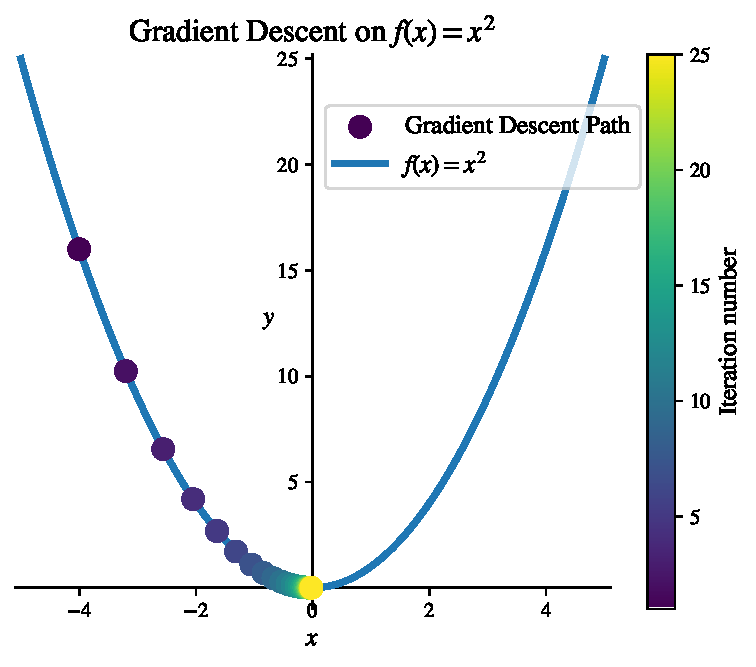
\includegraphics[width=0.68\textwidth]{figures/simple_gradient_descent_x^2.pdf}
    \caption{Gradient Descent on the function $f(x)=x^2$, starting from $x_0 = -4$ with $\eta = 0.01$, ran for 30 iterations.}
    \label{fig:simple_gradient_descent}
\end{figure}
For this simple example the iteration converged quickly, reaching an absolute value less than 0.001 after only 27 iterations. Gradient descent is not always this efficient. 

The two natural weaknesses of gradient descent are neatly explained in \textcite[p.~65--71]{MLRefined}. The first stems from the gradient always being perpendicular to the contour line. This is easily proved through parameterization.

\begin{lemma}
    Let $w(t)$ be a parametrization of a contour surface for a differentiable function $f: X^n \rightarrow Y$. Then $\nabla f \perp w(t)$. 
\end{lemma}

\begin{proof}
$$f(w(t)) = C \Rightarrow \frac{d}{dt} f(w(t)) = 0 \Rightarrow \nabla f(w(t)) \cdot \frac{\partial w(t)}{\partial t} = 0$$
The result follows from $\frac{\partial w(t)}{\partial t}$ being parallel to the contour
\end{proof}

This may lead to \textit{zig-zagging} behavior for ill conditioned problems, as seen in \autoref{fig:zigzagGradientDescent}.

\begin{figure}[H]
    \centering
    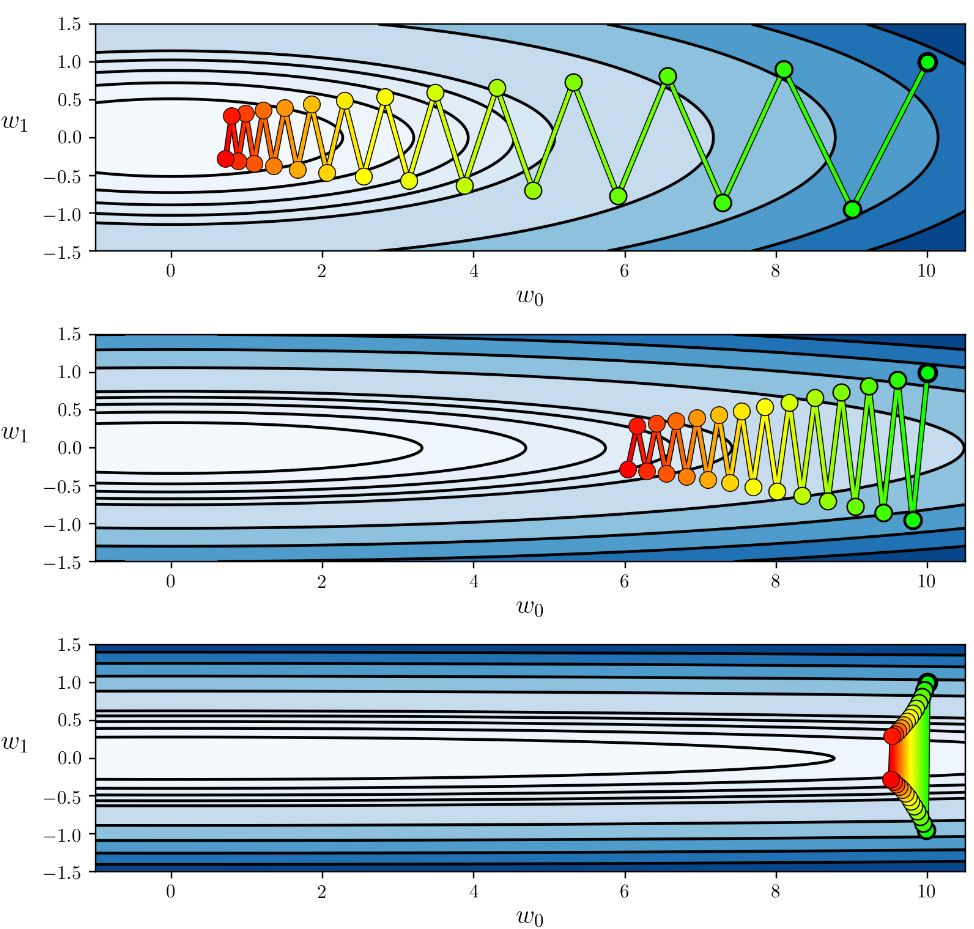
\includegraphics[width=0.9\textwidth]{Project2/figures/Gradient_descent_zigzag.jpeg}
    \caption{Figure 3.13 \parencite[p.~68]{MLRefined} illustrating the zig-zagging behavior
of gradient descent.}
    \label{fig:zigzagGradientDescent}
\end{figure}

The other challenge of gradient descent is its slow crawling behaviour in flatter regions of a function such as saddle points. This is nicely illustrated by 50 iterations with $\eta = 0.1$ on the function 
\begin{equation*}
    g(w) =  \max\{0, 1 + (3w - 2.3)^3\}^2 + \max\{0, 1 + (-3w + 0.7)^3\}^2,
\end{equation*}
as seen in \autoref{fig:CrawlGradientDescent}.

\begin{figure}[H]
    \centering
    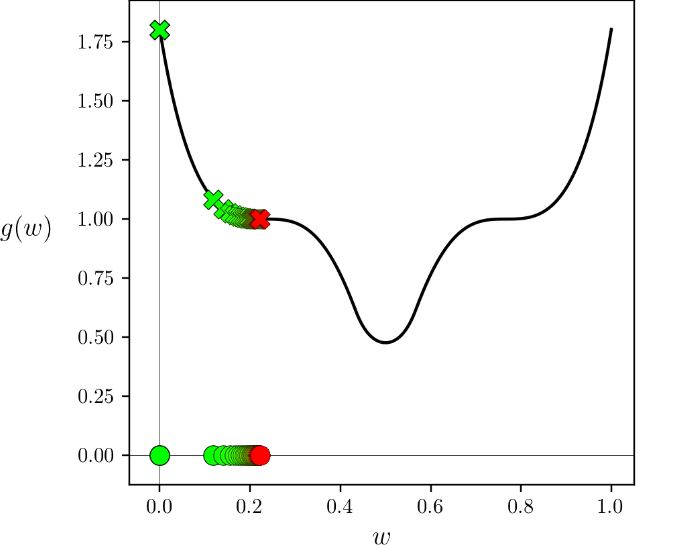
\includegraphics[width=0.7\textwidth]{Project2/figures/Gradient_descent_saddle_crawl.jpeg}
    \caption{Figure 3.14 from \parencite[p.~70]{MLRefined} illustrating the slow crawling behaviour of gradient descent.}
    \label{fig:CrawlGradientDescent}
\end{figure}

\begin{comment}
When performing gradient descent for machine learning the function we are minimizing is the cost function. A measure of the distance between predicted and observed outputs. It is important to note that this function is defined by 
\end{comment}

\subsubsection{Stochastic gradient descent}
Recall that the cost function is defined as a measurement of the distance between our predictions and the observed values. A large dataset can therefore quickly turn computationally expensive, if we were to compute the cost function and corresponding gradient for everything all at once. To combat this, we often apply \textit{Stochastic gradient descent} (SGD).

We first introduce batch gradient descent, where we split out dataset into \textit{batches} of size $M$. For each iteration, we compute the gradient for each batch individually, updating our estimate for each. Instead of computing the cost and corresponding gradient for all data points each time as in gradient descent, we thus only calculate it for a smaller subset, having the effect of requiring less iterations.

In stochastic gradient descent, we apply the same method, differing by drawing a sample of $M$ random points from our data set with replacement. The cost surface achieved by this is truly a different surface from the one achieved by using all the data points, but the number of features and thus the dimentionality, is the same. For this method to work we are banking on there being enough overlap between the samples such that the gradient is expected to point in the same direction when calculated for all data points.

It is common practice to organize our algorithm in a double loop. If we have $n$ samples in total, the inner loop iterates over $\lfloor\frac{M}{n} \rfloor$. That is the number of batches that fit in our dataset. The outer loop iterates over the number of epochs.

\newpage

\begin{algorithm}[hbt!]
\caption{Batch Gradient Descent}\label{alg:SGD}
\KwData{Dataset D={$x_1,...,x_n$}, Learning rate $\eta$, Batch Size M, No. of Epochs E}
\KwResult{Model Parameters w}
\For{i in range(E)}{
    batches = create\_batches(D, M)\;
  \For{j in range(n//M)}{
    batch = batches[j]\;
    gradient = compute\_gradient(batch, w)\;
    w = w - $\eta$ $\cdot$ gradient\;
  } 
}
\end{algorithm}
 
Let $\boldsymbol{x}_i$ be the $i$th batch for $i=1, \ldots, m$. We can rewrite (\ref{eq:gradient_descent}) as
\begin{align*}
        \boldsymbol{w}_{j+1} = \boldsymbol{w}_j - \eta_j\nabla f_i (\boldsymbol{x}_i)
\end{align*}
where $j=1,...,m \cdot \#epochs$. Notice that the gradient is indexed as it is defined from the data points in the batch.

As stated in the previous subsection, gradient descent finds the local minima $f(\boldsymbol{\xi})$ by exploration. This is beneficial for convex functions, or if the local minima is already known to be the global minima. For non-convex functions, or in the case where the global minima is not known (which is the case most of the time), SGD introduces more exploration. This means that instead of getting stuck in a local minima, by randomness, there is a higher probability of finding the global minima. SGD also have an added bonus that it is dependent on the batch size rather than the data set size. Thus the learning rate can still converge, even if the data set is large.

It is important to keep in mind that for the following descent methods we can define their corresponding stochastic counterparts in the same way as we did for gradient descent. And that gradient descent and stochastic gradient descent is sometimes used to refer to the family of optimizers and their stochastic counterparts.

\subsubsection{Momentum based gradient descent}
Momentum is an added parameter meant to address these issues of vanilla gradient descent. The iteration is defined as
\begin{equation}
\begin{aligned} 
    \boldsymbol{w}_{k+1} &= \boldsymbol{w}_k + \boldsymbol{v}_{t+1}, \\
    \boldsymbol{v}_{t+1} &= \rho \boldsymbol{v}_t - \eta \boldsymbol{g}_k, \qquad \boldsymbol{v}_0 = 0 
\end{aligned}
\label{eq:momentum_eq}
\end{equation}
$\boldsymbol{v}$ is called the velocity term and $\rho$ is the momentum parameter. $\rho$ can be thought of as the velocity's resistance to change while the learning rate $\eta$ characterizes the influence of the gradient. An intuitive analogy is to think of our descent algorithm as a particle moving on the surface we wish to minimize. The gradient is the force acting on our particle, $\eta$ is its amplifier, and $\rho$ is the mass of the particle. This way our particle might be able to roll past the saddle point in \autoref{fig:CrawlGradientDescent} and obtain a less ``zig-zaggy" path than in \autoref{fig:ZigZagMomentumGradientDescent}.

Here we see momentum gradient descent performed on the same ill conditioned problem as the first panel of \autoref{fig:zigzagGradientDescent} with $\rho$ equal to $0, 0.2, 0.7$ respectively.

\begin{figure}[H]
    \centering
    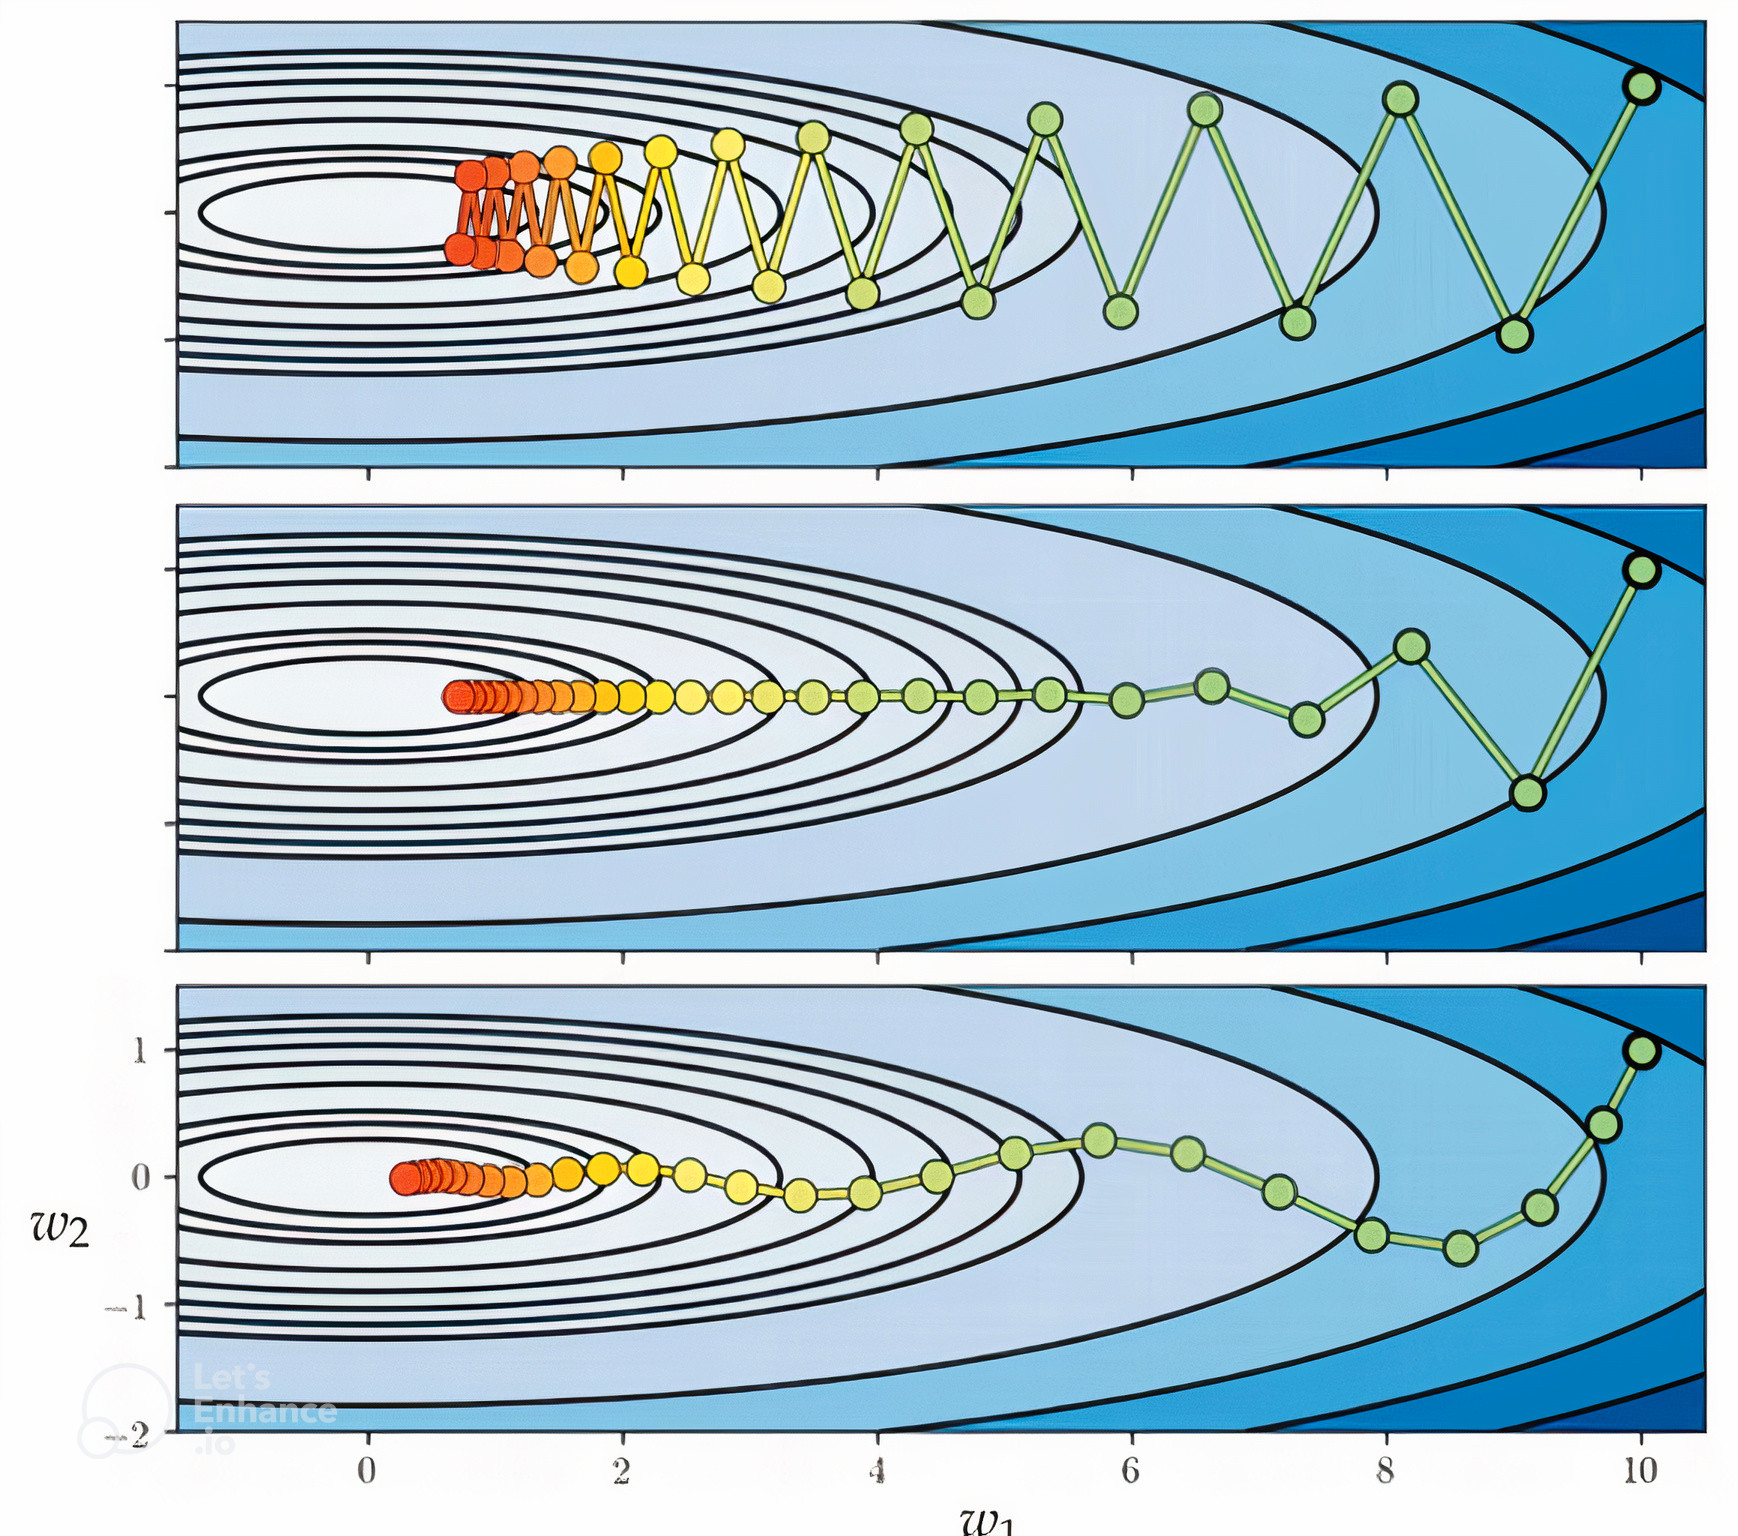
\includegraphics[width=0.8\textwidth]{Project2/figures/momentum_based_gradient_descent_less_zig.jpg.jpg}
    \caption{Figure A3 from \textcite[p.~478]{MLRefined}. The zig-zagging behavior of gradient descent can be ameliorated using the momentum-accelerated gradient descent}
    \label{fig:ZigZagMomentumGradientDescent}
\end{figure}


\subsubsection{AdaGrad}
The Adaptive gradient optimizer, or AdaGrad was introduced by \textcite{duchi2011adaptive} and its update rule is given by
\begin{equation*}
    \boldsymbol{w}_{k+1} = \boldsymbol{w}_{k} - \eta \diag\left( G_{k} \right)^{-1/2} \odot \boldsymbol{g}_k
\end{equation*}
where $\odot$ is the Hadamard product and $G_k$ is the sum of the outerproducts of the previous gradients
\begin{equation*}
    G_k = \sum_{i = 0}^k \boldsymbol{g}_i \boldsymbol{g}_i^T.
\end{equation*}

We thus have that $\diag\left(G_{k}\right)^{(n)}$ (the $n^{th}$ component of $\diag\left(G_k\right)$) is the sum of the squares of the previous gradients in direction $n$
\begin{equation*}
    \diag\left(G_{k}\right)^{(n)} = \sum_{i=0}^k  \left(g_k^{(n)}\right)^2 .
\end{equation*}
Normally a small numerical stabiliser is added to $G_k$ to avoid division by zero, giving us
\begin{equation*}
    \boldsymbol{w}_{k+1}^{(n)}= \boldsymbol{w}_{k}^{(n)}- \frac{\eta}{\sqrt{\delta + \diag \left( G_{k} \right)^{(n)}}} \odot g_k^{(n)}.
\end{equation*}

As $\diag\left(G_k\right)^{(n)}$ increases, the step size in direction $n$ decreases, which reduces the emphasis on that particular direction as it is traversed. This is the core concept of AdaGrad's design. AdaGrad is most effective when two conditions are met: first, when we need to move the same distance in each dimension, and second, when we have an appropriate choice of $\eta$. Opting for a too small $\eta$ could result in the algorithm converging very slowly or coming to a halt due to the decaying step size. Conversely, selecting a too large $\eta$ could lead to sluggish convergence. Thus, selecting an appropriate value of $\eta$ is vital to ensuring efficient functioning of the algorithm. 

\subsubsection{RMSprop}
RMSprop, root mean square propagation, was first introduced in 2012, in lecture 6 of the Coursera course ``Neural Networks for Machine Learning" by Geoff Hinton
\parencite{NNforML-Lecture6}. It's update rule is defined as 

\begin{align*}
    \boldsymbol{v}_{k+1} =& \rho \boldsymbol{v}_{k} + (1-\rho) \boldsymbol{g}_k^{\circ 2}\\
    w_{k+1}^{(n)} =& w_k^{(n)} - \frac{\eta}{  \sqrt{\delta + v_{k+1}^{(n)}}} g_k^{(n)}
\end{align*}
where $^{\circ 2}$ is the Hadamard power defined by $\boldsymbol{x}^{\circ 2} = \boldsymbol{x} \odot \boldsymbol{x}$.

We have chosen to only give the element wise update rule, as the vector notation for the final equation is not very pretty for RMSprop. $\delta$ is a numerical stabilizer, $0 \leq \rho \leq 1$ and $\boldsymbol{v}_0$ is usually initialised to the zero vector.

Like AdaGrad, the update keeps some sort of memory of previous gradients. Where $\rho$ can be thought of as the strength of the memory, i.e. how much of the previous iterations should impact the next. This allows for some of the same benefits as AdaGrads decaying learning rate.

\subsubsection{ADAM}
Adaptive moment estimation, most commonly known as ADAM, is an optimization algorithm which combines some of the aspects from RMSprop with momentum. It's update is given by
\begin{align*}
    \boldsymbol{m}_{k+1} =& \frac{\rho_1 \boldsymbol{m}_k + (1- \rho_1) \boldsymbol{g}_k}{\left(1 - \rho_1^{k+1}\right)}\\
    \boldsymbol{v}_{k+1} =& \frac{\rho_2 \boldsymbol{v}_k + (1-\rho_2) \boldsymbol{g}_k^{\circ 2}}{\left(1-\rho_2^{k+1}\right)}\\
    w_{k+1}^{(n)} =& w_k^{(n)} - \frac{\eta}{ \sqrt{\delta+v_{k+1}^{(n)}}} m_{k+1}^{n},
\end{align*}
where $0 \leq \rho_1,\rho_2 < 1$.

Notice that the denominator of $\boldsymbol{m}_{k+1}$ and $\boldsymbol{v}_{k+1}$ starts somewhere in $(0,1]$ and then increases to 1 as $k \to \infty$. This gives an amplification of $\boldsymbol{m}_k$ and $\boldsymbol{v}_k$, which subsides for larger $k$. This is meant to alleviate a bias towards zero as $\boldsymbol{m}_0, \boldsymbol{v}_0 = 0$ \parencite[Section 3]{kingma2014adam}.
\label{AdamAmp}.
%It may be tempting to conclude that every subsequent algorithm is superior to its predecessor. However, this is not strictly true.
% \vspace{2mm}
Optimization algorithms can be used to minimize any specific function. However, the latter three are all designed for minimizing a particular set of functions; the cost functions of Artificial Neural Networks (ANNs). These cost functions measure the error made by ANNs in predicting observed values from input data. How these predictions are made and adjusted is the topic of section 2.4

\subsubsection{Time-based decay}
Time-based decay removes the need for the user to fix the learning rate $\eta$ themselves. Here, the rate is adjusted automatically based on the number of iterations computed, and two hyperparameters $t_0$ and $t_1$. It is defined simply by
\begin{equation}\label{eq:TimeDecay}
    \eta = \frac{t_0}{e \cdot M + m + t_1},
\end{equation}
where $e$ is the number of epochs passed, $M$ is the size of batches, and $m$ is the number of minibatches computed in the current epoch. Thus the earlier iterations are given higher priority, as $\eta \to 0$ as $e \to \infty$, with $\eta = \frac{t_0}{t_1}$ for the first iteration.

\subsection{Neural Networks}
Neural networks are computational systems inspired by the networks of neurons within the brain. In the brain, when a neuron receives an electrical impulse above a certain threshold, it sends an electrical signal to the neurons connected to it, causing a chain reaction. In order to mimic this, an artificial neural network is set up with a number of layers, each with a set of artificial neurons. The first layer is commonly called the input layer, which is followed by a number of hidden layers, culminating in the final layer called the output layer.

\begin{figure}[ht]
\centering
\def\layersep{2.5cm}
\def\nodeinlayersep{1.2cm}
\begin{tikzpicture}[shorten >=1pt,->,draw=black!50, node distance=\layersep]
    \tikzstyle{every pin edge}=[<-,shorten <=1pt]
    \tikzstyle{neuron}=[circle, fill=black!25,minimum size=20pt,inner sep=0pt]
    \tikzstyle{input neuron}=[neuron, fill=red!50];
    \tikzstyle{output neuron}=[neuron, fill=orange!50];
    \tikzstyle{hidden neuron}=[neuron, fill=blue!50, minimum size=20pt];
    \tikzstyle{hidden neuron2}=[neuron, fill=blue!50, minimum size=20pt];

    \foreach \name / \y in {0,...,2}
        \node[input neuron] (I-\name) at (0,-\y) {};

    \foreach \name / \y in {0,...,3}
        \path[yshift=0.5cm]
            node[hidden neuron] (H1-\name) at (\layersep,-\y cm) {};

    \foreach \name / \y in {0,...,3}
        \path[yshift=0.5cm]
            node[hidden neuron2] (H2-\name) at (2*\layersep,-\y cm) {};    

    \foreach \name / \y in {0,...,1}
        % \node[output neuron,pin={[pun edge={->}]right:Output \#\y}, right of=H2-2] (O-\name) at (3*\layersep, -\y cm) {};
        \path[yshift=-0.5cm]
            node[output neuron] (O-\name) at (3*\layersep, -\y cm) {};


    \foreach \source in {0,...,2}
        \foreach \dest in {0,...,3}
            \path (I-\source) edge (H1-\dest);

    \foreach \source in {0,...,3}
        \foreach \dest in {0,...,3}
            \path (H1-\source) edge (H2-\dest);

    \foreach \source in {0,...,3}
        \foreach \dest in {0,...,1}
            \path (H2-\source) edge (O-\dest);
\end{tikzpicture}
\caption{Illustration of a fully connected feed-forward neural network with an input layer (red), two hidden layers (blue) and an output layer (orange).}
\label{fig:SimpleFFNN}
\end{figure}

The \textit{feed-forward} neural network (FFNN), was one of the first, and perhaps simplest, artificial neural network. Each node is connected to nodes in the next layer, with a weight $w \in \mathbb{R}$ attached to each edge, representing the strength of the connection between them. Additionally, we attach a bias $b \in \mathbb{R}$ to the node itself, also refereed to as the offset. Henceforth, we describe the \textit{fully connected} feed-forward neural network, where the nodes are connected to \textit{all} nodes in the next layer, illustrated in \autoref{fig:SimpleFFNN}.


Information in this network moves from left to right. The value of a node is dependent on the weights and values of the previous layer, as well as the bias. Let $N_l \in \mathbb{N}$ be the number of nodes in layer $l$ with the input layer being $l = 0$. We then calculate
\begin{equation*}
    z_{i}^1 = \sum_{j = 0}^{N_0 - 1} w_{ij}^1 x_j + b_i^1 \qquad \textnormal{for} \ i = 0, 1, \ldots, N_1 - 1,
\end{equation*}
with $w^l_{ij}$ being the weight connecting node $i$ in layer $l$ and node $j$ in layer $l-1$, $b_i^l$ the bias of node $i$ and $x_j$ the $j^{th}$ input. We call $z$ the activation value. Let $f^l: \mathbb{R} \to \mathbb{R}$ be a function, called the activation function for the $l^{\text{th}}$ layer. We calculate the output of the node by $a_i^l = f^l(z_i^l)$. For the following layers, we calculate a \textit{feed-forward pass}
\begin{equation*}
    a_i^l = f^l(z_{i}^l) = f^l \left( \sum_{j = 0}^{N_l - 1} w_{ij}^l a_j^{l-1} + b_i^{l} \right) \qquad \textnormal{for} \ i = 0, 1, \ldots, N_l - 1,
\end{equation*}
illustrated in \autoref{fig:FeedForward}.

\begin{figure}[ht]
\centering
\def\layersep{3cm}
\def\nodeinlayersep{2cm}
\begin{tikzpicture}[shorten >=1pt,->,draw=black!50, node distance=\layersep]
    \tikzstyle{every pin edge}=[<-,shorten <=1pt]
    \tikzstyle{neuron}=[circle, fill=black!25,minimum size=25pt,inner sep=0pt]
    \tikzstyle{input neuron}=[neuron, fill=red!50];
    \tikzstyle{output neuron}=[neuron, fill=orange!50];
    \tikzstyle{hidden neuron}=[neuron, fill=blue!50];

    % Input nodes
    \foreach \name / \y in {0,...,1}
        \node[input neuron] (I-\name) at (0,-\y * \nodeinlayersep) {$x_\y$};

    % Hidden layer
    \foreach \name / \y in {0,...,1}
        \node[hidden neuron] (H-\name) at (\layersep,-\y * \nodeinlayersep) {$a_\y^1$};

    % Output node
    \path[yshift=-0.5 * \nodeinlayersep]
        node[output neuron] (O-0) at (2*\layersep, 0 cm) {$a_0^2$};

    \path[->] 
        % Weights from first input
        (I-0) edge [->] node [midway, above] {$w^1_{0, 0}$} (H-0)
        (I-0) edge [->] node [midway, above] {$w^1_{0, 1}$} (H-1)
        % Weights from second input
        (I-1) edge [->] node [midway, below] {$w^1_{1, 0}$} (H-0)
        (I-1) edge [->] node [midway, below] {$w^1_{1, 1}$} (H-1)
        % Weights to output
        (H-0) edge [->] node [midway, above] {$w^2_{0, 0}$} (O-0)
        (H-1) edge [->] node [midway, below] {$w^2_{1, 0}$} (O-0);

    
    \foreach \source in {0,...,1}
        \foreach \dest in {0}
            \path (H-\source) edge (O-\dest);

    \path[->]
        (H-0) edge [loop above] node [above] {$f\left(z_0^1\right)$} ()
        (H-1) edge [loop below] node [below] {$f\left(z_1^1\right)$} ()
        (O-0) edge [loop above] node [above] {$f\left(z_0^2\right)$} ();

    \node (BH-0) at (0.5*\layersep,  0.5*\nodeinlayersep) {$b_0^1$};
    \node (BH-1) at (0.5*\layersep, -1.5*\nodeinlayersep) {$b_1^1$};
    \node (BO-0) at (1.5*\layersep, -0.5*\nodeinlayersep) {$b_0^2$};

    \path[->]
        (BH-0) edge (H-0)
        (BH-1) edge (H-1)
        (BO-0) edge (O-0);
\end{tikzpicture}
\caption{Illustration of a feed-forward pass in a neural network with two inputs (red), two hidden nodes (blue), and one output node (orange).}
\label{fig:FeedForward}
\end{figure}

We gather the weights connecting the $l^{th}$ and $(l-1)^{th}$ layers in a $N_{l} \times N_{l-1}$ matrix $\mathbf{W}_l$, and the biases and outputs in $N_l \times 1$ column vectors $\mathbf{b}_l, \mathbf{y}_l$ as follows.
\begin{equation*}
    \mathbf{W}_l = 
    \begin{bmatrix}
        w_{0,0} & w_{0,1} & \ldots & w_{0,N_{l-1}} \\
        w_{1,0} & w_{1,1} & \ldots & w_{1,N_{l-1}} \\
        \vdots & \vdots & \ddots & \vdots \\
        w_{N_{l},0} & w_{N_{l},1} & \ldots & w_{N_{l},N_{l-1}} \\
    \end{bmatrix}
    \qquad
    \mathbf{b}_l =
    \begin{bmatrix}
        b_0^l \\ b_1^l \\ \vdots \\ b_{N_l}^l
    \end{bmatrix}
    \qquad
    \mathbf{y}_l =
    \begin{bmatrix}
        y_0^l \\ y_1^l \\ \vdots \\ y_{N_l}^l
    \end{bmatrix}
\end{equation*}
We can then simplify the summation to get $\mathbf{z}_l = \mathbf{W}_l \mathbf{y}_{l-1} + \mathbf{b}_l$. We then extend the function $f^l: \mathbb{R} \to \mathbb{R}$ to the function $F^l: \mathbb{R}^{N_l \times 1} \to \mathbb{R}^{N_l \times 1}$ by defining
\begin{equation*}
    F^l(\boldsymbol{x}) = \left[ f^l \left( x_0 \right), \ f^l \left( x_1 \right), \ \ldots, \ f^l \left( x_{N_l - 1} \right) \right]^T,
\end{equation*}
such that the function operates elementwise. For simplicity, this function $F^l$ will also be notated $f^l$.

We define the realization of our neural network as the function $\mathcal{N}: \mathbb{R}^{N_0 \times 1} \to \mathbb{R}^{N_h \times 1}$, with $h$ being the output layer as
\begin{equation*}
    \mathcal{N}(\boldsymbol{x}) =
    f^h\left(
    \mathbf{W}_h f^{h-1} \left(
    \mathbf{W}_{h-1}f^{h-2} \left(\ldots f^1\left( \mathbf{W}_1 \boldsymbol{x} + \mathbf{b}_1 \right) \right)
    + \mathbf{b}_{h-1} \right) 
    + \mathbf{b}_h \right).
\end{equation*}
Defining the function $\mathcal{A}^l: \mathbb{R}^{N_{l-1} \times 1} \to \mathbb{R}^{N_{l}}$ as the function
\begin{equation*}
    \mathcal{A}^l (\boldsymbol{x}) = \mathbf{W}_l \boldsymbol{x} + \mathbf{b}_l,
\end{equation*}
we can simplify our notation by noting that $\mathcal{N}$ is a composition of functions
\begin{align*}
    \mathcal{N} &= f^h \circ \mathcal{A}^h \circ f^{h-1} \circ \mathcal{A}^{h-1} \circ \ldots \circ f^1 \circ \mathcal{A}^1 \\
    &= \bigcirc_{i = 1}^h f^{i} \circ \mathcal{A}^{i}.
\end{align*}

The Universal Approximation Theorem states that a neural network with even a single hidden layer, can approximate a continuous function on a compact subset arbitrarily well with an arbitrary number of hidden nodes given a fitting choice for the activation function \parencite{universalapprox}. The proof of this theorem falls outside the scope of this project, but we highly recommend i.e. \textcite{Guliyev2015ASH} or \textcite{universalapprox} if you have a passing interest in analysis. As we will see, our choice of activation function matters greatly.

\subsubsection{Activation functions}
For the sake of brevity, we restrict our self to one activation function for the hidden layers, and one for the output layer. To motivate our choice of activation function, we begin with the definition of a linear operator from real analysis \parencite[p.~150]{lindstrom2017spaces}.

\begin{definition}
    Assume that $V$ and $W$ are two vector spaces over $\mathbb{R}$. A function $A: V \to W$ is called a \textit{linear operator} (or a \textit{linear map}) if it satisfies:
    \begin{enumerate}[label=(\roman*)]
        \item $A(\alpha\boldsymbol{u}) = \alpha A(\boldsymbol{u}$) for all $\alpha \in \mathbb{R}$ and $\boldsymbol{u} \in V$.

        \item $A(\boldsymbol{u} + \boldsymbol{v}) = A(\boldsymbol{u}) + A(\boldsymbol{v})$ for all $\boldsymbol{u}, \boldsymbol{v} \in V$.
    \end{enumerate}
\end{definition}

\begin{theorem}[Composition of linear operators]
    Assume that $U, V, W$ are vector spaces over $\mathbb{R}$ and that $A: U \to V$, $B: V \to W$ are linear operators. Then $B \circ A$ is a linear operator.
    \label{thm:Linear}
\end{theorem}
\begin{proof}
    Let $\boldsymbol{u}, \boldsymbol{v} \in V$, $\alpha, \beta \in \mathbb{R}$. Then
    \begin{align*}
        B(A(\alpha \boldsymbol{u} + \beta \boldsymbol{v})) &= B(\alpha A(\boldsymbol{u}) + \beta A(\boldsymbol{v}))
        = \alpha B(A(\boldsymbol{u})) + \beta B(A(\boldsymbol{v})),
    \end{align*}
    showing that $B \circ A$ is indeed a linear operator.
\end{proof}

Due to \autoref{thm:Linear}, if we were to choose a linear activation function for the hidden layer, $\mathcal{N}$ would just be a composition of linear operators, and therefore be linear itself. We would then not get any benefit from adding multiple hidden layers, as it could just be represented as one linear operation. This greatly restricts the hypothesis space, which is why we opt for non-linear activation functions \parencite[p.~72]{CholletFrancois2018DlwP}.
% \parencite[p.~72]{CholletFranccois2018DlwP}

A common choice, and the one first presented in \textcite{universalapprox}, is a so called sigmoidal function $\sigma$. A sigmoidal function is a function $\sigma: \mathbb{R} \to \mathbb{R}$ which satisfies
\begin{equation*}
    \lim_{t \to +\infty} \sigma(t) = 1 \qquad \textnormal{and} \qquad \lim_{t \to -\infty} \sigma(t) = 0.
\end{equation*}
A simple function which satisfies this, is the $(0,1)$-clip function, defined by
\begin{equation*}
    f(x) = 
    \begin{cases}
        1 & \textnormal{for } x \geq 1 \\
        x & \textnormal{for } x \in (0,1) \\
        0 & \textnormal{for } x \leq 0
    \end{cases}.
\end{equation*}
The most common choice however is perhaps the standard logistic function \parencite{jentzen2023mathematical}, often just called the sigmoid function, defined by
\begin{equation*}
    f(x) = \frac{1}{1 + e^{-x}}.
\end{equation*}
Both of these functions are clearly sigmoidal, illustrated in the plot in \autoref{fig:sigmoid}.

\begin{figure}[ht]
    \centering
    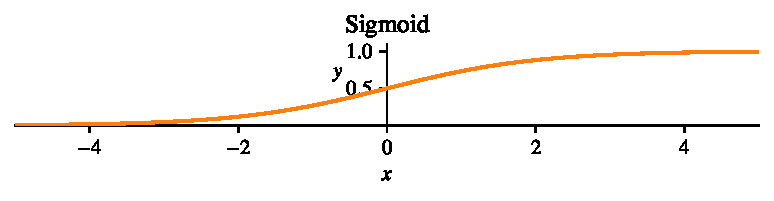
\includegraphics[width=.7\textwidth]{activators/sigmoid.pdf}
    \caption{A plot of the sigmoid and $(0,1)$-clip activation functions on $[-4, 4]$.}
    \label{fig:sigmoid}
\end{figure}

% However, the activation functions do not have to be sigmoidal in order to satisfy the requirements for the Universal Approximation Theorem. In fact, it is enough to require that the activation function is non-polynomial \parencite{nonpolynomial}. (\small{venter på svar fra Morten, virker for godt til å være sant}) 

Another commonly used activation function is the rectified linear unit (ReLU), defined by
\begin{equation*}
    f(x) = \max(0, x) = \frac{x + |x|}{2} =
    \begin{cases}
        x & \textnormal{if } x \geq 0 \\
        0 & \textnormal{if } x < 0
    \end{cases}.
\end{equation*}
However, this function suffers from what some call dying ReLUs, where nodes in effect die by outputting constant $0$. To combat this, we introduce the leaky rectified linear unit (LReLU), defined by
\begin{equation*}
    f(x) =
    \begin{cases}
        x & \textnormal{if } x \geq 0 \\
        \gamma x & \textnormal{if } x < 0
    \end{cases}.
\end{equation*}
for some positive $\gamma \in \mathbb{R}$. These functions are illustrated in \autoref{fig:LRELU}.

\begin{figure}[ht]
    \centering
    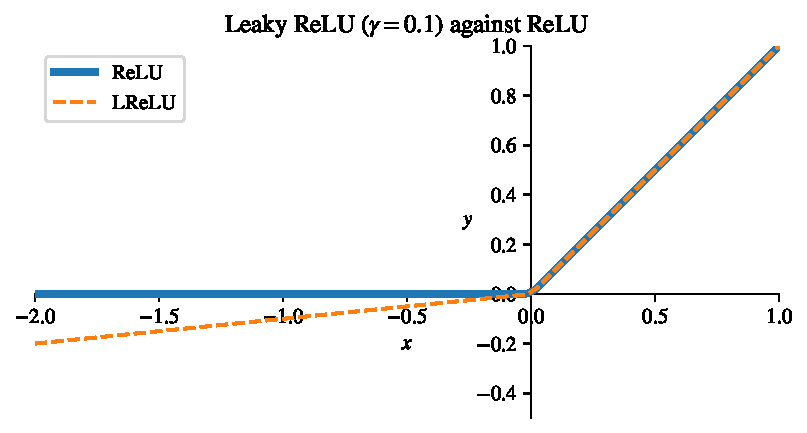
\includegraphics[width=.7\textwidth]{activators/LReLU.pdf}
    \caption{A plot of leaky rectified linear unit (LReLU) activation function on $[-2, 1]$, with $\gamma=0.1$, against ReLU.}
    \label{fig:LRELU}
\end{figure}

Two other important functions that are particularly used on the output layer for multi-class classification problems, are the $\argmax$ and $softmax$ functions.

The $\argmax$ function delivers the index or position associated with the highest value from a numeric input vector. If  each node in the output layer denotes the models predicted probability of an input being classified in the corresponding class, it becomes clear that the $\argmax$ function essentially provides the predicted class or classification. This function is however not differentiable and therefore is not suited for training. Which will be clear by section 2.3.2.

The $softmax$ function is used to convert any vector to a valid discrete probability distribution. It is given by
\[
softmax(\textbf{z}) = \begin{bmatrix}
\frac{e^{z_1}}{\sum_i e^{z_i}} \\
\vdots \\
\frac{e^{z_n}}{\sum_i e^{z_i}}
\end{bmatrix} = \textbf{a}
\]
It keeps the sorted order of the input vector. That is if $z_i < z_j$ then $a_i < a_j$. It also satisfies
\[
\sum_{i=1}^n a_i = 1
\]



\subsubsection{Minimizing the cost function: Backpropagation}

Backpropagation serves as the heart of model optimization. As the name implies, it involves a backwards pass through our Artificial Neural Network (ANN). To understand its operation, we need to consider a model, referred to here as $\mathcal{N}$. After computing the output for a given input variable, $\boldsymbol{x}$, denoted by $\mathcal{N}(\boldsymbol{x})$, it becomes inherently natural to assess the performance of our model. Specifically, we want to compute the loss emerging from deviations between the model's output and the expected values

\[
L(\mathcal{N}(\boldsymbol{x}), \mathbf{y})
\]
The mean over $n$ such losses gives us the cost function
\[
C(\mathcal{N}, \boldsymbol{x}^*, \mathbf{y}^*) = \frac{1}{n} \sum_{i=0}^{n}L(\mathcal{N}(\boldsymbol{x}^{(i)}), \mathbf{y}^{(i)})
\]
Here we let $\mathbf{x}^*$ and $\mathbf{y}^*$ denote the matrices containing the column vectors $\mathbf{x}^{(i)}$ and $\mathbf{y}^{(i)}$. These matrices are commonly referred to as our labeled data or our training data. This cost function is our optimization problem, the function we wish to minimize. 

\[
\argmin_{\mathcal{N}} C(\mathcal{N}, \boldsymbol{x}^*, \mathbf{y}^*) 
\]
$\mathcal{N}$ consists of three components: our weights, biases and activation functions. Minimizing with respect to the activation functions is not necessary, as by the Universal Approximation Theorem, there are many that will suffice. By minimizing with respect to the weights and biases we get the back propagation algorithm.

Letting $\eta$ and $\mu$ encompass all the different learning rates by our methods in section 2.2 we get the general iteration on layer $l$
\begin{align*}
    \hat{w_{i,j}^{l}} =\hspace{1mm}&
    w_{i,j}^{l} - \eta \frac{\partial C}{\partial {w_{i,j}^{l}}}\\
    \hat{b_i^{l}} =\hspace{1mm}& b_i^{l} - \mu  \frac{\partial C}{\partial b_i^l} 
\end{align*}

Here we are taking some notational liberty in the use of partial derivatives. As we'll see these are functions of the weights, the pre-activated and the activated values of the network, and are of course evaluated at the current values for a iteration. 

 We return to $a_i^l$ begin the value of node $i$ in layer $l$ and $z_i^l$ the value before activation. Then for some arbitrary layer $l$ we get, by the chain rule

\begin{align}
    \frac{\partial C}{\partial w_{i,j}^l} =& \frac{\partial C}{\partial a_i^l} \frac{\partial f^l}{\partial z_i^l} \frac{\partial z_i^l}{\partial w_{i,j}^l} \label{eq:1} 
    \\
    \frac{\partial C}{\partial b_i^l} = & \frac{\partial C}{\partial a_i^l} \frac{\partial f^l}{\partial z_i^l} \frac{\partial z_i^l}{\partial b_i^l} \label{eq:2} 
\end{align}
The third factors of these products simplifies to

\begin{align}
    \frac{\partial z_{i}^l }{\partial w_{i,j}^l} = &  \frac{\partial}{\partial w_{i,j}^l} \sum_{k = 0}^{N_l - 1} w_{i,k}^L a_k^{l-1} + b_i^l = a_j^{l-1} \label{eq:3} \\
    \frac{\partial z_i^l}{\partial b_i^l} = &  1 \label{eq:4} 
\end{align}

\noindent
The second, $\frac{\partial f^l}{\partial z_i^l}$ can simplified to $f^{l'}(z_i^l)$ whenever the activation function $f^l$ is a function of just one variable. 


\begin{figure}[ht]
\centering
\def\layersep{2.5cm}
\def\nodeinlayersep{1.2cm}
\begin{tikzpicture}[shorten >=1pt,->,draw=black!50, node distance=\layersep]
    \tikzstyle{every pin edge}=[<-,shorten <=1pt]
    \tikzstyle{neuron}=[circle, fill=black!25,minimum size=20pt,inner sep=0pt]
    \tikzstyle{hidden neuron}=[neuron, fill=blue!50, minimum size=20pt];
    \tikzstyle{hidden neuron2}=[neuron, fill=blue!50, minimum size=20pt];
    \tikzstyle{hidden neuron opaque}=[neuron, fill=blue, minimum size=20pt, opacity=0.2];  % New style for opaque neurons


    \foreach \name / \y in {1}
        \path[yshift=0.5cm]
            node[hidden neuron] (H1-\name) at (\layersep,-\y cm) {$a^l_i$};

    \foreach \name / \y in {0,2,3} 
        \path[yshift=0.5cm]
            node[hidden neuron opaque] (H1-\name) at (\layersep,-\y cm) {};

    \foreach \name / \y in {0,...,3}
        \path[yshift=0.5cm]
            node[hidden neuron2] (H2-\name) at (2*\layersep,-\y cm) {};    

    % Labels for the layers
    \node[above of=H1-0, node distance=11mm] (label1) {$l$};
    \node[above of=H2-0, node distance=11mm] (label2) {$l+1$};

     \node[above of=H1-0, node distance=7mm] (label1) {$\vdots$};
    \node[above of=H2-0, node distance=7mm] (label2) {$\vdots$};
    \node[below of=H1-3, node distance=7mm] (label1) {$\vdots$};
    \node[below of=H2-3, node distance=7mm] (label2) {$\vdots$};

    \foreach \source in {1}
        \foreach \dest in {0,...,3}
            \path (H1-\source) edge (H2-\dest);

\end{tikzpicture}
\caption{Illustration of Connections from one Neuron in a Neural Network}
\label{fig:Connections}
\end{figure}

\noindent
To see how $\frac{\partial C}{\partial a_i^l}$ expands. Consider \autoref{fig:Connections}. A change in $a_i^l$ will trickle down to the next layer. For a single edge we get
\[
\frac{\partial C}{\partial a_i^{l+1}} \frac{\partial a_j^{l+1}}{\partial a_i^l} =  \frac{\partial C}{\partial a_i^{l+1}} \frac{\partial f^{l+1}}{\partial z_j^{l+1}} w_{i,j}^{l+1}
\]

Summation over all the edges gives us $\frac{\partial C}{\partial a_i^l}$


\begin{align}
    \frac{\partial C}{\partial a_i^l} =  \sum_{i=0}^{N_{l+1}-1} \frac{\partial C}{\partial a_i^{l+1}} \frac{\partial f^{l+1}}{\partial z_j^{l+1}} w_{i,j}^{l+1} \label{eq:5} 
\end{align}


If $l$ is the final layer in the network $\frac{\partial C}{\partial a_i^l}$ is the partial derivative with respect to the multivariate function $C$ - no more chain rule with respect to other nodes.

Combining equation \eqref{eq:1} with \eqref{eq:3} and \eqref{eq:2} with \eqref{eq:4}. We get

\begin{align}
     \frac{\partial C}{\partial w_{i,j}^l} =& \frac{\partial C}{\partial a_i^l} \frac{\partial f^l}{\partial z_i^l} a_j^{l-1}\label{eq:6} 
    \\
    \frac{\partial C}{\partial b_i^l} = & \frac{\partial C}{\partial a_i^l} \frac{\partial f^l}{\partial z_i^l} \label{eq:7} 
\end{align}
Equations \eqref{eq:5} through \eqref{eq:7} form the backbone of the backpropagation algorithm. As we observe, equation \eqref{eq:5}, which is integral to both \eqref{eq:6} and \eqref{eq:7}, relies on the partial derivatives of the proceeding layer. After computing the forward pass and storing all the relevant network values, we can initiate the backpropagation process, moving from right to left, one layer at the time. This systematic approach allows us to calculate all the gradients necessary for our optimization algorithms.


\subsubsection{Automatic Differentiation}
Automatic Differentiation (AD), also known as algorithmic differentiation or computational differentiation, refers to a set of techniques to numerically evaluate partial derivatives. It differs from symbolic differentiation and numerical differentiation.

At a high level, automatic differentiation leverages the principle that any computational calculation, regardless of its complexity, carries out a series of basic arithmetic tasks (like addition, subtraction, multiplication, and division) and fundamental functions (such as exp, log, sin, cos, etc.). Every one of these functions are stored as separate variables. For instance our computation might encounter the expression $sin(a+b)$, where $a,b$ are two of the input variables. This could be stored as $h_1$. Furthermore $a+b$ could be stored as $h_2$. This gives 

\[
\frac{\partial h1}{\partial a} =  \frac{\partial h1}{\partial h2} \frac{\partial h2}{\partial a}
\]
\[
\frac{\partial h1}{\partial b} =  \frac{\partial h1}{\partial h2} \frac{\partial h2}{\partial b}
\]
Just as we did for backpropagation!

This way we can find all the partial derivatives with respect to any of the input variables by repeatedly applying the chain rule \parencite{walther2007automatic} . This method is not only very precise but also efficient. It does however, require added storage, in the worst case growing proportionally with number of operations in the function.
\parencite{baydin2018automatic}

The use of automatic differentiation techniques is most relevant for the calculation of $\frac{\partial C}{\partial a_i^L}$ for the final layer. As a single pass of reverse accumulation AD (the process briefly explained above) allows us to calculate the partial derivatives with respect to the entire layer $a^L$


\subsubsection{Derivative of Binary Cross Entropy with respect to weights}
Recall the Loss and BCE cost function given by

\[
L(y, p) = -ylog(p) - (1-y)log(1-p)
\]

\[
C(\mathbf{y}, \mathbf{p}) = \frac{1}{n} \sum_{i=1}^{n} L(y_i, p_i)
\]


Let's look at the loss function first.
\[
\frac{\partial L(y,p)}{\partial p} = \frac{-y}{p} + \frac{1-y}{1-p} 
\]
For binary classification it's common to use the sigmoid as our activation function for the final layer to obtain a valid probability. Giving $\sigma(z) = p$ as the derivative is given by
\[
\sigma'(x) = \sigma(x)(1-\sigma(x))
\]
We get 

\begin{align*}
\frac{\partial L(y,p)}{\partial z} =& \frac{\partial L(y,p)}{\partial p} \frac{\partial p}{\partial z} \\
=& \left(\frac{-y}{p} + \frac{1-y}{1-p}\right) \left(p(1-p)\right)\\
=& -y(1-p) + (1-y)p\\
=& \hspace{1mm} p-y 
\end{align*}

Thus for the cost function with respect to the final layer of weights we get


\begin{align*}
    \frac{C}{\partial \mathbf{w^L}}  =& \hspace{1mm} \frac{\partial C}{\partial \mathbf{p}} \frac{\partial \mathbf{p}}{\partial \mathbf{w^L}} \odot \mathbf{w^L}
    \\
    =& \hspace{1mm} \frac{1}{n} \left( \mathbf{p} - \mathbf{y}\right) \odot \mathbf{w^L}
\end{align*}

This analytical expression is very convenient for backpropagation.


\newpage
\section{Method}
In order to verify that our methods work, we began with testing our gradient descent code with the polynomial
\begin{equation}\label{eq:simplepoly}
    f(x) = 4 - 3x + 2x^2.
\end{equation}
With this, we can more easily visualize and understand the difference between the various methods. We generated our data with 100 values for $\boldsymbol{x}_i \in N(0, 1)$, and added noise $\boldsymbol{\varepsilon}_i \in N(0, 1)$ to our values such that $\boldsymbol{y} = f(\boldsymbol{x}) + \boldsymbol{\varepsilon}$ seen in \autoref{fig:input_values}. Utilizing polynomial regression, our design matrix was then
\begin{equation}
    X = \begin{bmatrix}
        1 & x_0 & x_0^2 \\
        1 & x_1 & x_1^2 \\
        & \vdots & \\
        1 & x_{100} & x_{100}^2
    \end{bmatrix},
    \label{eq:design}
\end{equation}
seeking to find $\boldsymbol{\theta} = [\theta_0, \theta_1, \theta_2]^T$ minimizing our cost function. We utilized both OLS and Ridge regression, applying both the analytical derivative and automatic differentiation.

\begin{figure}[ht]
    \centering
    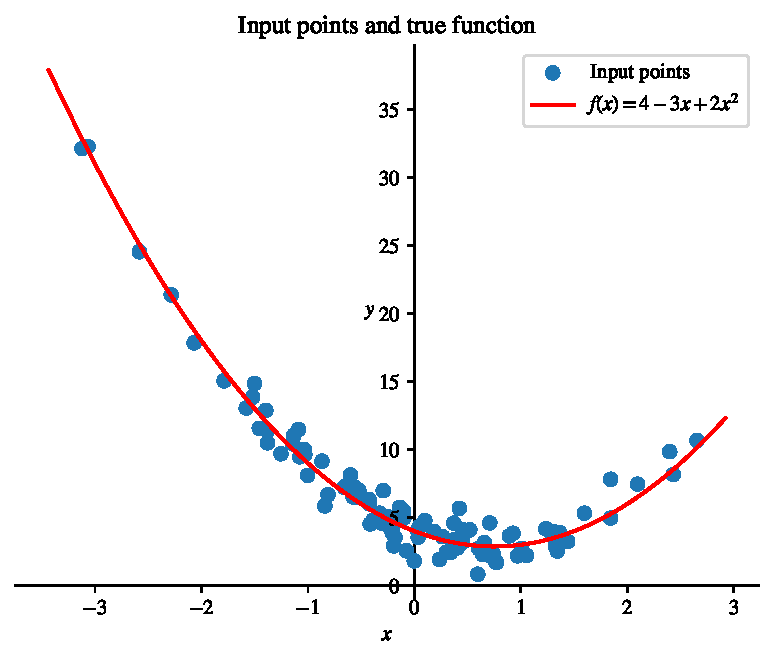
\includegraphics[width=0.7\textwidth]{Project2/figures/polynomial_grad/input_points.pdf}
    \caption{Values used for verifying gradient descent on $f(x) = 4 - 3x + 2x^2$.}
    \label{fig:input_values}
\end{figure}

With a better understanding of how gradient descent with the various methods works, we moved on to regression with a neural network. Here, we utilized Franke's function, defined by
\begin{equation*}
    \begin{split}
        f(x,y) & = \frac{3}{4}\exp\left(-\frac{(9x-2)^2}{4} - \frac{(9y-2)^2}{4}\right) + \frac{3}{4}\exp\left(-\frac{(9x+1)^2}{49} - \frac{(9y+1)}{10}\right) \\
        & + \frac{1}{2}\exp\left(-\frac{(9x-7)^2}{4} - \frac{(9y-3)^2}{4}\right) - \frac{1}{5}\exp\left(-(9x-4)^2 - (9y-7)^2\right).
    \end{split}
\end{equation*}
for $x,y \in [0,1]$. A major advantage with regression through the neural network is that we do not have to transform our inputs to a polynomial as in (\ref{eq:design}), instead allowing the network to learn the behaviour through the hidden layers. This has the advantage of not coaxing the network into fitting a polynomial. We therefore have only two input nodes for $x$ and $y$, with one output node outputting the predicted height $z$. We used 100 evenly spaced points in $[0,1]$ for our values of $x$ and $y$, transforming our inputs to a mesh grid giving $100 \times 100$ points.

For classification, we used the original Wisconsin Breast Cancer Dataset \parencite{breastcancerwisonsin}, attempting to predict from measurements of tumours whether they are malignant or benign. The dataset consists of 9 features, being labeled either 2 for benign or 4 for malignant. We transform the labels with $f(x) = x / 2 - 1$ such that the labels are binary. There are 699 data points, however 16 of them are missing some data and are thus excluded from our analysis.

There are several different ways to initialize the weights and biases of ANNs; nonetheless we chose random initialization. Our weights are sampled from a normal distribution with mean zero and standard deviation 1. Conversely our weights are drawn from a narrower distribution, with the same mean, but a standard deviation of 0.01.

\subsection{The code}
Our original implementation primarily used \verb|NumPy| for the linear algebra and \verb|autograd| for automatic differentiation. Due to computational concerns, it was then rewritten to primarily rely on \verb|JAX| \parencite{jax2018github}, which is a Google developed library combining \verb|XLA| and \verb|autograd| designed for high-performance computing. This has the advantage of being a lot faster, however leads to more verbose code. As an example, consider the sigmoid function implemented in \verb|JAX| and \verb|NumPy|.

\begin{minted}{python}
from jax import lax, jit
import numpy as np

@jit
def sigmoid_jax(X):
    return lax.reciprocal(lax.add(1.0, lax.exp(-X)))

def sigmoid_numpy(X): # NumPy equivalent
    return 1 / (1 + np.exp(-X))
\end{minted}

Note that we apply the \verb|@jit| decorator to enable just-in-time compilation, which is a leading factor in the speedup. The sigmoid function is also a built-in function in \verb|JAX| under the name \verb|lax.logistic|, however we chose to use our own implementation to keep everything in the same style.

As \verb|jit| works poorly with classes, requiring methods to be completely functional in order to assure correct functionality, we chose to extract the most costly computations into their own functions, using pure python primarily for higher level bookkeeping. One of the trickier parts of porting to \verb|JAX| was that it has no built in method for elementwise differentiation. Thus to differentiate the hidden functions, which are performed elementwise, we used the following code.

\begin{minted}{python}
from jax import grad, vmap
from autograd import elementwise_grad

def derivate_jax(func):
    return vmap(vmap(grad(func)))

def derivate_autograd(func): # autograd equivalent
    return elementwise_grad(func)
\end{minted}

As we are working with column vectors in $\mathbb{R}^{n \times 1}$, we have to apply two vectorizing maps. If \verb|f|$: \mathbb{R}^{n \times 1} \to \mathbb{R}^{n \times 1}$, then \verb|vmap(f)|$: \mathbb{R}^{1} \to \mathbb{R}^{1}$. Lastly, note that \verb|JAX| treats vectors of dimension \verb|(1,)| differently from scalars, so we have to apply a final vectorizing map to achieve our desired result of \verb|vmap(vmap(f))|:$\mathbb{R} \to \mathbb{R}$ as \verb|grad| only works on scalar-output functions.

To be able to structure our code better, we developed a simple package which can be installed with \mintinline{bash}{pip3 install .} in the Project2 directory. Note that there seems to be a bug in \verb|JAX| where anything smaller than $10^{-7}$ is rounded to $0$ when using \verb|jit|.

\newpage
\section{Results}
We generated a large number of plots, however we found it excessive to add everything here. The remaining figures are available on \href{https://github.com/augustfe/FYSSTK}{GitHub}.


\subsection{Analysis of univariate polynomial}
We began with the very simple case of attempting to fit (\ref{eq:simplepoly}) using Gradient Descent with a constant learning rate, with OLS as our cost function.
\begin{figure}[ht]%
    \centering
    \subfloat[\centering Analytical derivative of OLS.]{{\includegraphics[width=5.5cm]{Project2/figures/polynomial_grad/OLS_analytic/constant_thetas.pdf} }}%
    \qquad
    \subfloat[\centering Automatic differentiation of OLS.]{{\includegraphics[width=5.5cm]{Project2/figures/polynomial_grad/OLS_autodiff/constant_thetas.pdf} }}%
    \caption{Model parameters $\theta$ for varying degrees of a constant learning rate $\eta$, using ordinary least squares with Gradient Descent. Run over 500 epochs.}%
    \label{fig:GDconstanttheta}%
\end{figure}
\begin{figure}[ht]%
    \centering
    \subfloat[\centering Analytical derivative of OLS.]{{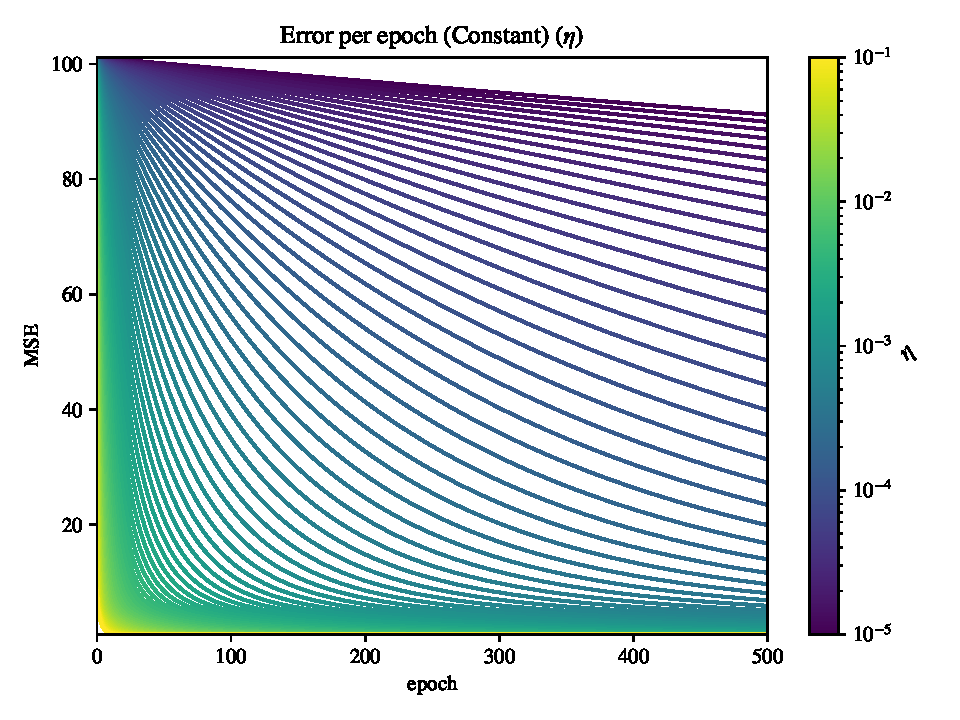
\includegraphics[width=5.5cm]{Project2/figures/polynomial_grad/OLS_analytic/constant_error.pdf} }}%
    \qquad
    \subfloat[\centering Automatic differentiation of OLS.]{{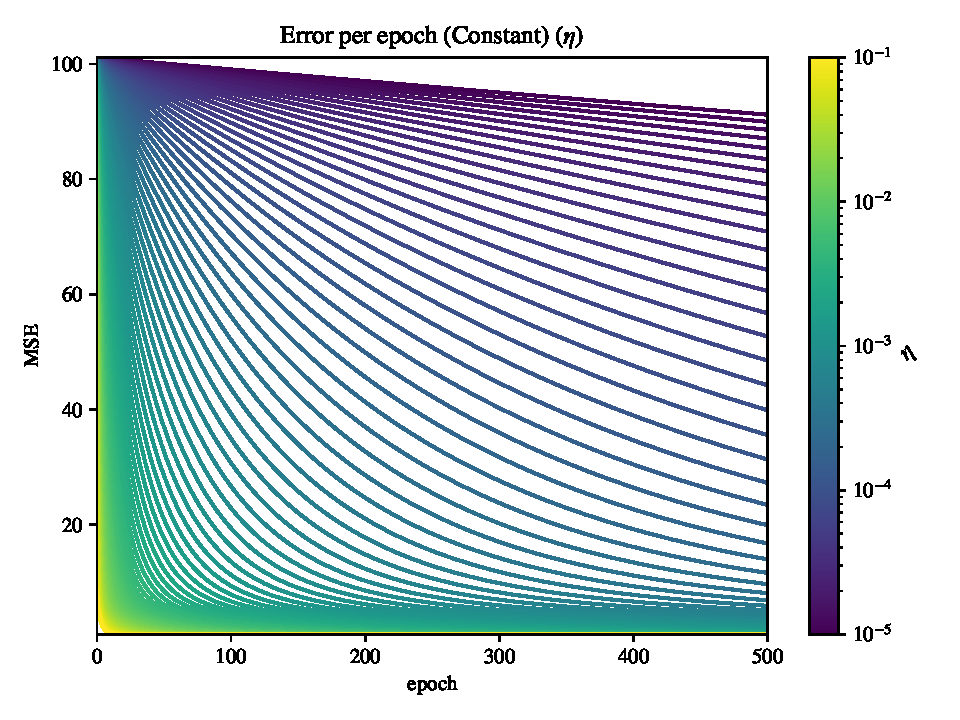
\includegraphics[width=5.5cm]{Project2/figures/polynomial_grad/OLS_autodiff/constant_error.pdf} }}%
    \caption{MSE of Gradient Descent with OLS over epochs for varying values of $\eta$.}%
    \label{fig:GDconstanterror}%
\end{figure}

As we see in \autoref{fig:GDconstanttheta} and \autoref{fig:GDconstanterror}, we get identical results using automatic differentiation and the analytical expression. We found the same results across the board, and the results using the analytic expressions will therefore be excluded from this section for the sake of brevity. In \autoref{fig:GDconstantpred} we see how Gradient Descent fits the target polynomial, predicting it almost perfectly for higher learning rates.

\begin{figure}[H]%
    \centering
    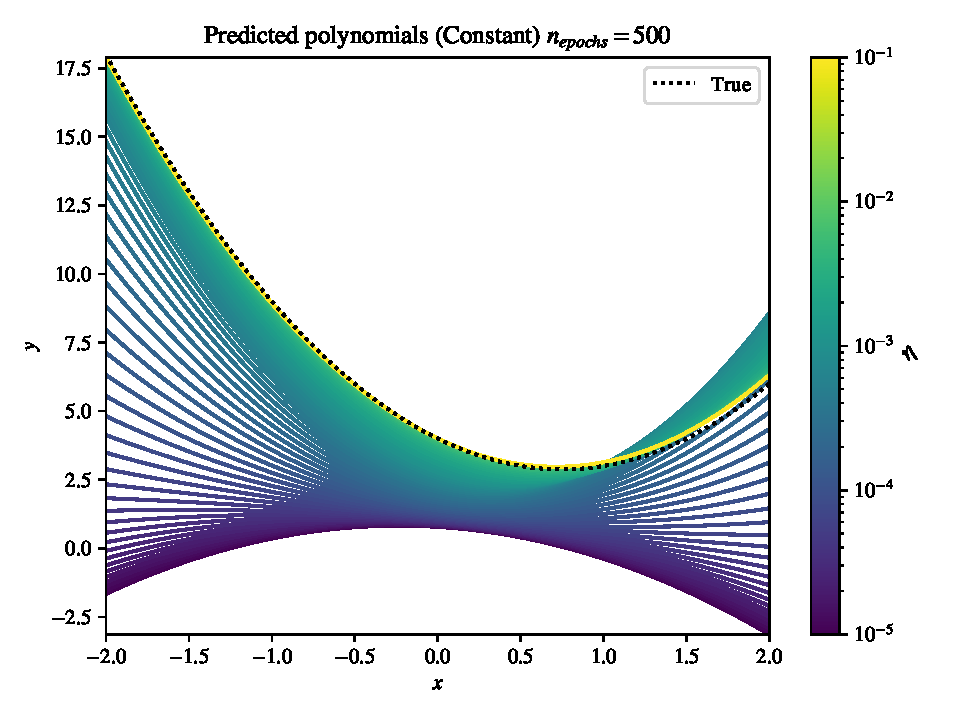
\includegraphics[width=8cm]{Project2/figures/polynomial_grad/OLS_autodiff/constant_prediction.pdf}
    \caption{Predicted polynomials for the resulting parameter values $\boldsymbol{\theta}$ from Gradient descent with constant learning rate after 500 epochs.}
    \label{fig:GDconstantpred}
\end{figure}

Introducing momentum, as in (\ref{eq:momentum_eq}) to our model can greatly improve results. We begin by seeing how the behaviour in \autoref{fig:ZigZagMomentumGradientDescent} is seen in our case.

\begin{figure}[H]%
    \centering
    \subfloat[\centering Error for varying $\rho$.]{{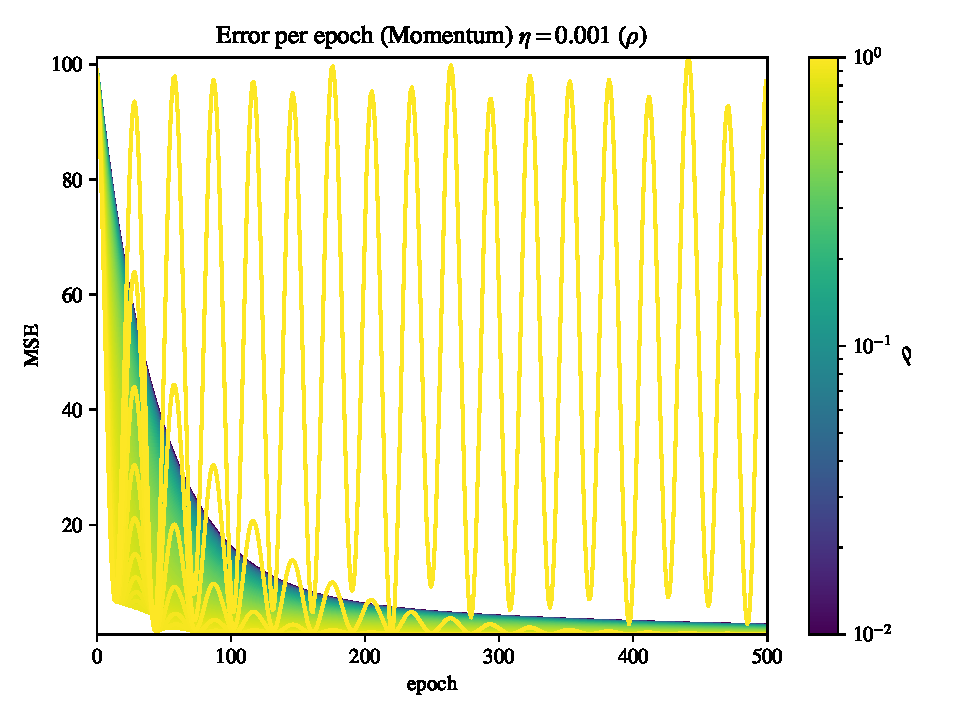
\includegraphics[width=5.5cm]{Project2/figures/polynomial_grad/OLS_analytic/momentum_error_rho.pdf} }}%
    \qquad
    \subfloat[\centering Parameters $\theta$ for varying $\rho$.]{{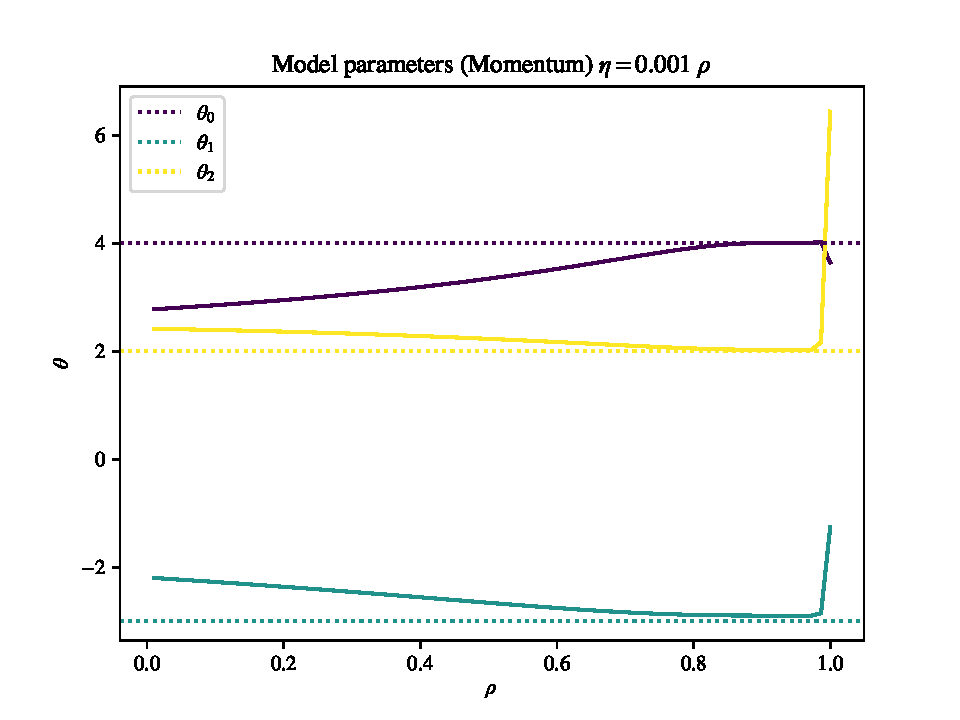
\includegraphics[width=5.5cm]{Project2/figures/polynomial_grad/OLS_autodiff/momentum_thetas_rho.pdf} }}%
    \caption{Gradient descent with varying momentum values $\rho$ over 500 epochs with a learning rate of $\eta = 10^{-3}$.}%
    \label{fig:GDmomentumrho}%
\end{figure}

As we see in \autoref{fig:GDmomentumrho}, we get greatly improved convergence results with higher values of $\rho$, although we have to be careful as we approach $\rho = 1$ as it can become quite unstable. Due to this, we settle for a value of $\rho = 0.9$ for the rest of our exploration.

\begin{figure}[H]%
    \centering
    \subfloat[\centering Error for varying $\eta$.]{{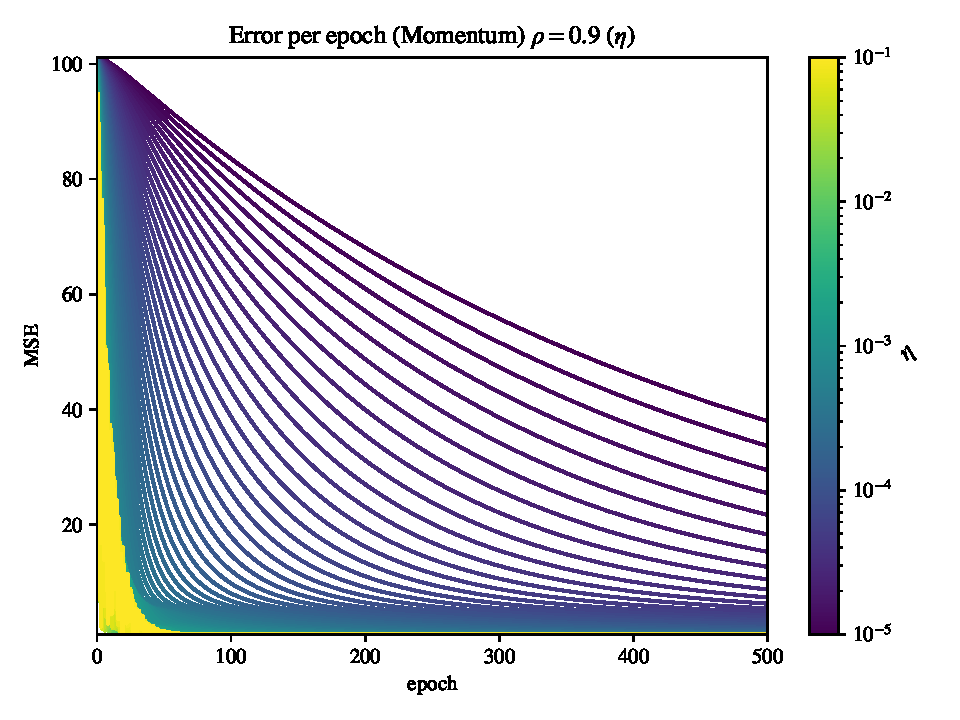
\includegraphics[width=5.5cm]{Project2/figures/polynomial_grad/OLS_analytic/momentum_error_eta.pdf} }}%
    \qquad
    \subfloat[\centering Parameters $\theta$ for varying $\eta$.]{{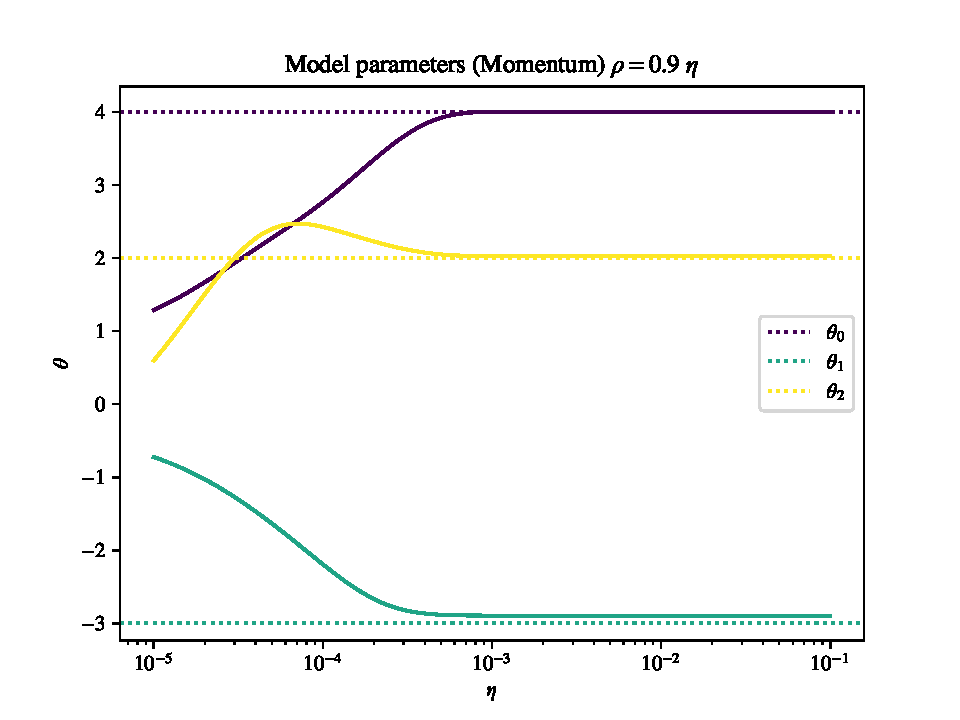
\includegraphics[width=5.5cm]{Project2/figures/polynomial_grad/OLS_autodiff/momentum_thetas_eta.pdf} }}%
    \caption{Gradient descent with momentum $\rho=0.9$ over 500 epochs with varying $\eta$.}%
    \label{fig:GDmomentumeta}%
\end{figure}

\begin{figure}[H]%
    \centering
    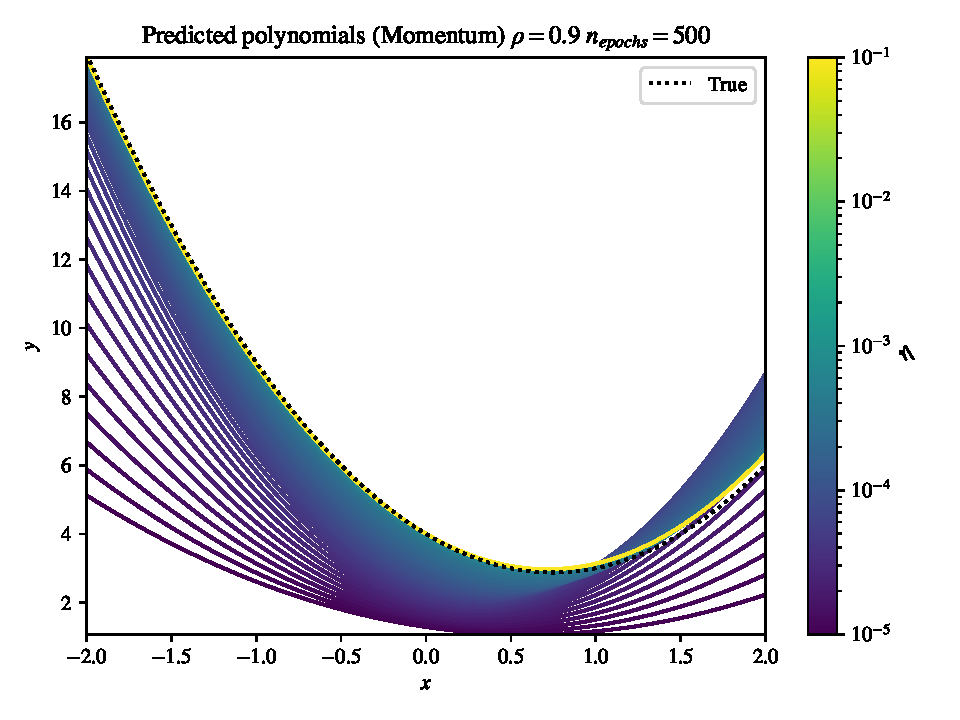
\includegraphics[width=8cm]{Project2/figures/polynomial_grad/OLS_autodiff/momentum_prediction_eta.pdf}
    \caption{Predicted polynomials for the resulting parameter values $\boldsymbol{\theta}$ from Gradient Descent with momentum after 500 epochs.}
    \label{fig:GDmomentumpred}
\end{figure}

In \autoref{fig:GDmomentumeta} and \autoref{fig:GDmomentumpred} we now see convergence for much smaller values of $\eta$. In \autoref{fig:GDmomentumheatmap} we see what a great effect our choice of $\rho$ has, both converging faster and becoming more unstable for higher values. Note the extremely skewed range of $\rho$, generated with $\arctan$ to highlight the details for higher values.

\begin{figure}[H]%
    \centering
    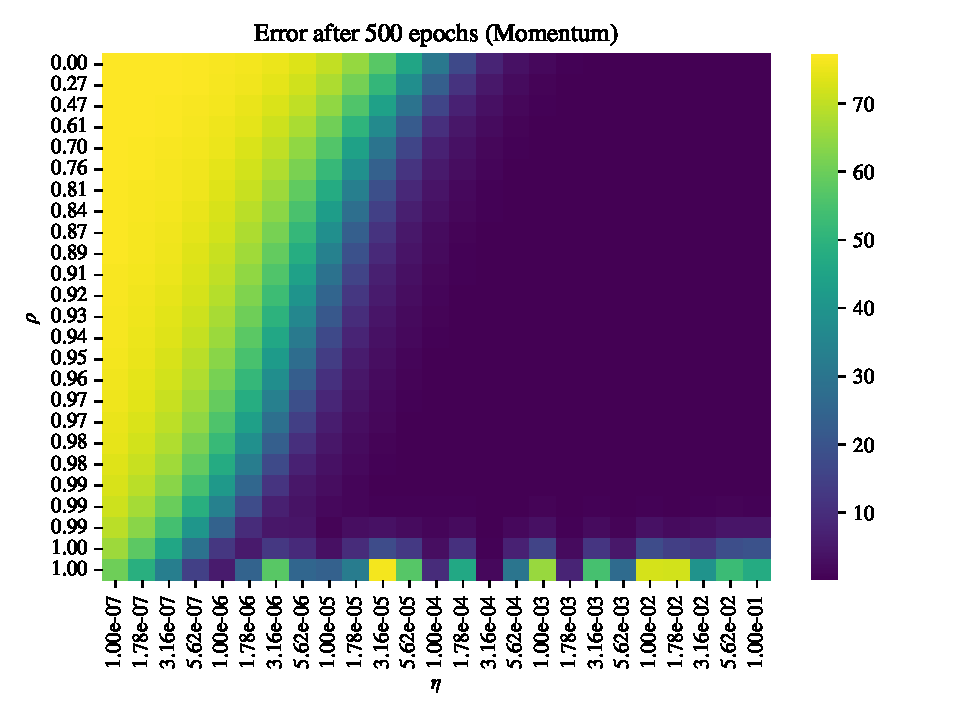
\includegraphics[width=8cm]{Project2/figures/polynomial_grad/OLS_autodiff/momentum_heatmap_eta_rho.pdf}
    \caption{Heatmap of error after 500 epochs for varying momentum values $\rho$ and learning rates $\eta$.}
    \label{fig:GDmomentumheatmap}
\end{figure}

\begin{figure}[H]%
    \centering
    \subfloat[\centering Error for varying $\eta$.]{{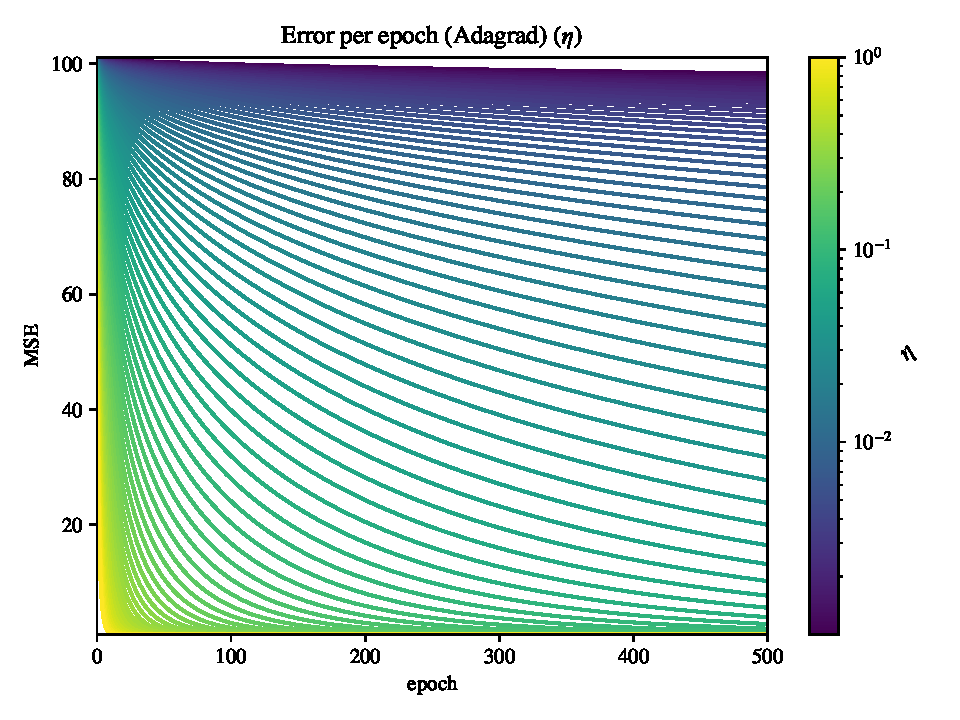
\includegraphics[width=5.5cm]{Project2/figures/polynomial_grad/OLS_analytic/adagrad_error.pdf} }}%
    \qquad
    \subfloat[\centering Parameters $\theta$ for varying $\eta$.]{{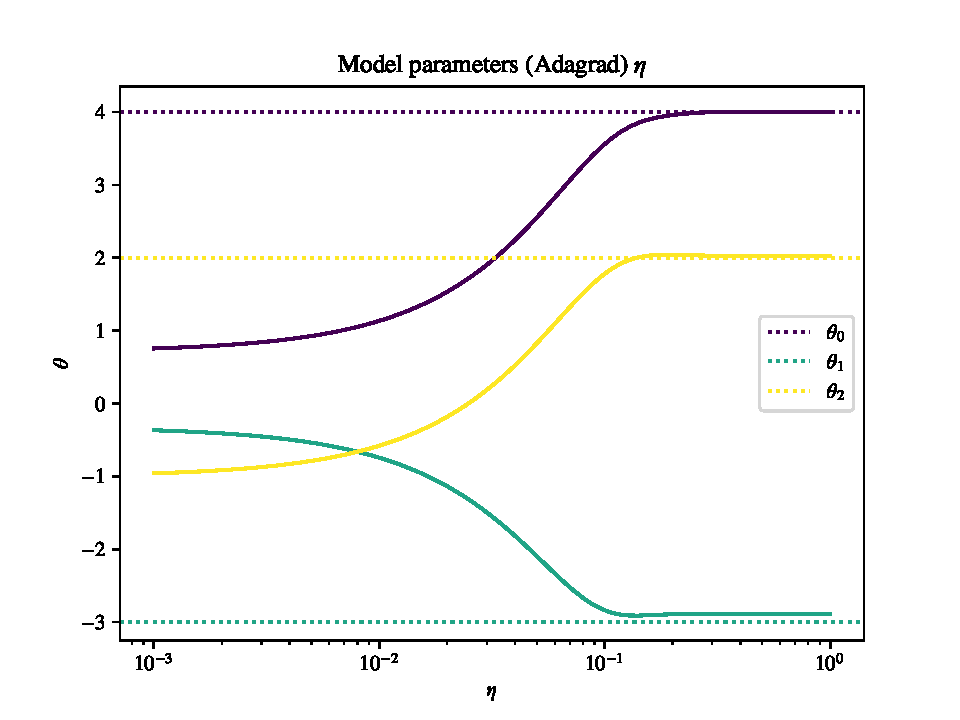
\includegraphics[width=5.5cm]{Project2/figures/polynomial_grad/OLS_autodiff/adagrad_thetas.pdf} }}%
    \caption{Gradient descent with Adagrad over 500 epochs with varying $\eta$.}%
    \label{fig:GDadagrad}%
\end{figure}

In \autoref{fig:GDadagrad} we see that Adagrad is considerably less sensitive to our choice of $\eta$, and it is interesting to note that we see the expected behaviour of Adagrad adjusting each parameter, removing the peak for $\theta_2$ seen previously, and being much more uniform. This is seen in \autoref{fig:GDadagradpred}, and note that it does not \textit{overshoot} the target.

\begin{figure}[H]%
    \centering
    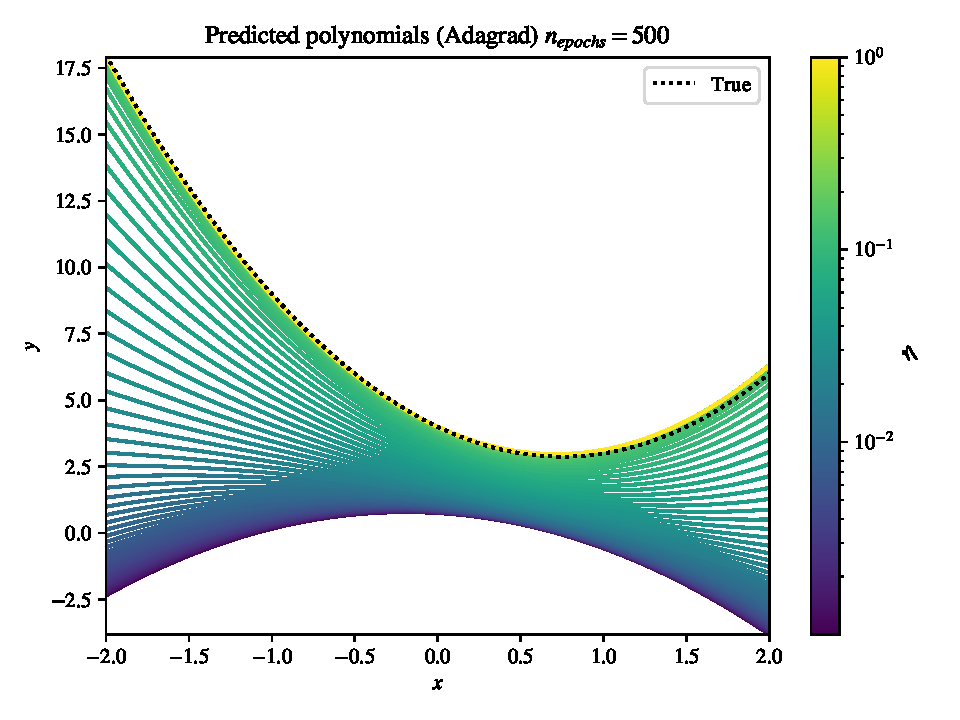
\includegraphics[width=8cm]{Project2/figures/polynomial_grad/OLS_autodiff/adagrad_prediction.pdf}
    \caption{Predicted polynomials for the resulting parameter values $\boldsymbol{\theta}$ using Adagrad after 500 epochs.}
    \label{fig:GDadagradpred}
\end{figure}

Introducing momentum leads to the same tendencies seen previously, seen in \autoref{fig:GDadagradmomentumeta}, \autoref{fig:GDadagradmomentumrho} and \autoref{fig:GDadagradmomentumheatmappred}.

\begin{figure}[H]%
    \centering
    \subfloat[\centering Error for varying $\eta$.]{{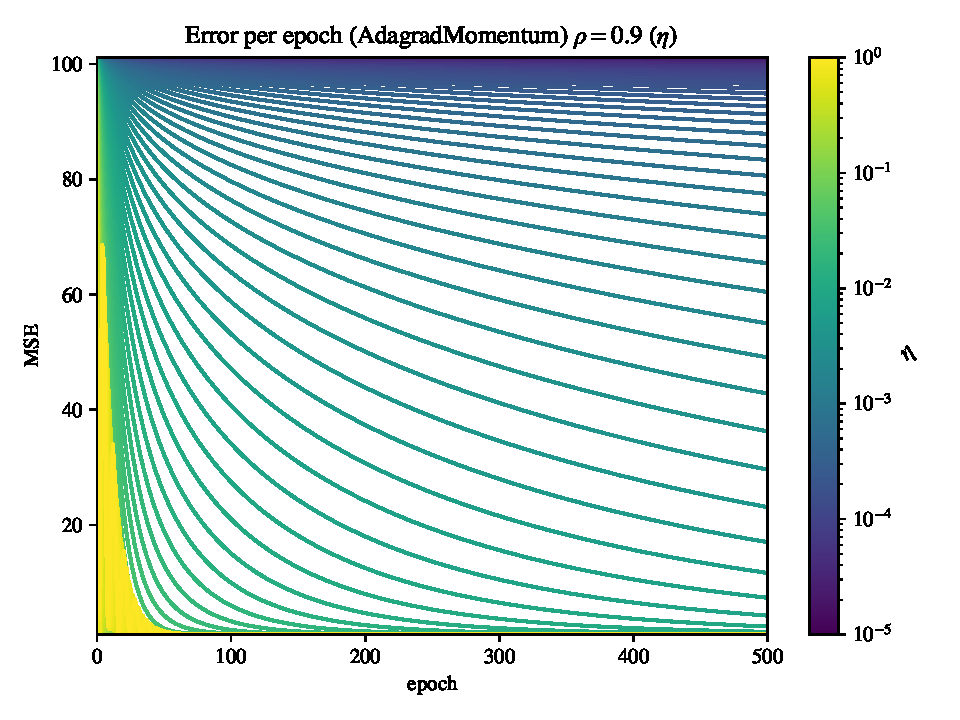
\includegraphics[width=5.5cm]{Project2/figures/polynomial_grad/OLS_autodiff/adagrad_momentum_error_eta.pdf} }}%
    \qquad
    \subfloat[\centering Parameters $\theta$ for varying $\eta$.]{{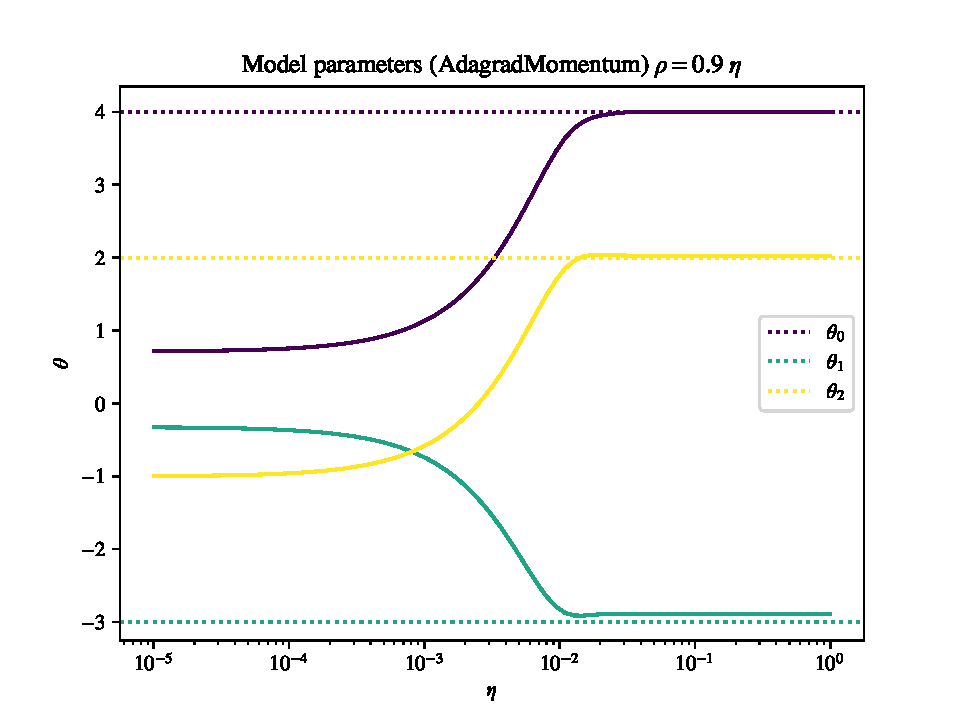
\includegraphics[width=5.5cm]{Project2/figures/polynomial_grad/OLS_autodiff/adagrad_momentum_thetas_eta.pdf} }}%
    \caption{Gradient descent with Adagrad Momentum over 500 epochs with varying $\eta$, $\rho=0.9$.}%
    \label{fig:GDadagradmomentumeta}%
\end{figure}

\begin{figure}[H]%
    \centering
    \subfloat[\centering Error for varying $\rho$.]{{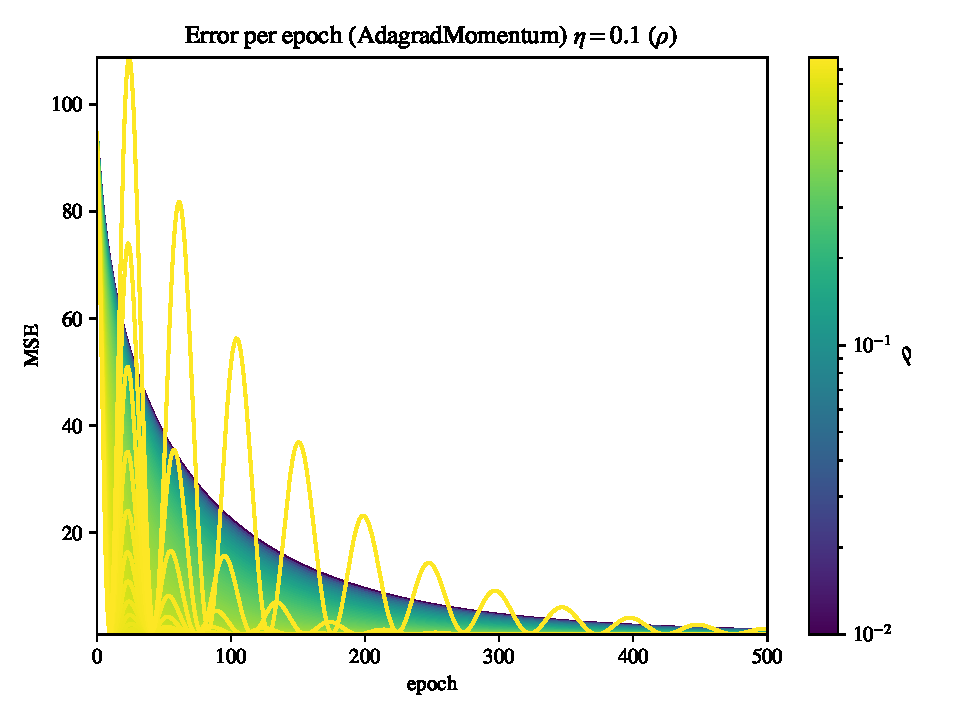
\includegraphics[width=5.5cm]{Project2/figures/polynomial_grad/OLS_autodiff/adagrad_momentum_error_rho.pdf} }}%
    \qquad
    \subfloat[\centering Parameters $\theta$ for varying $\rho$.]{{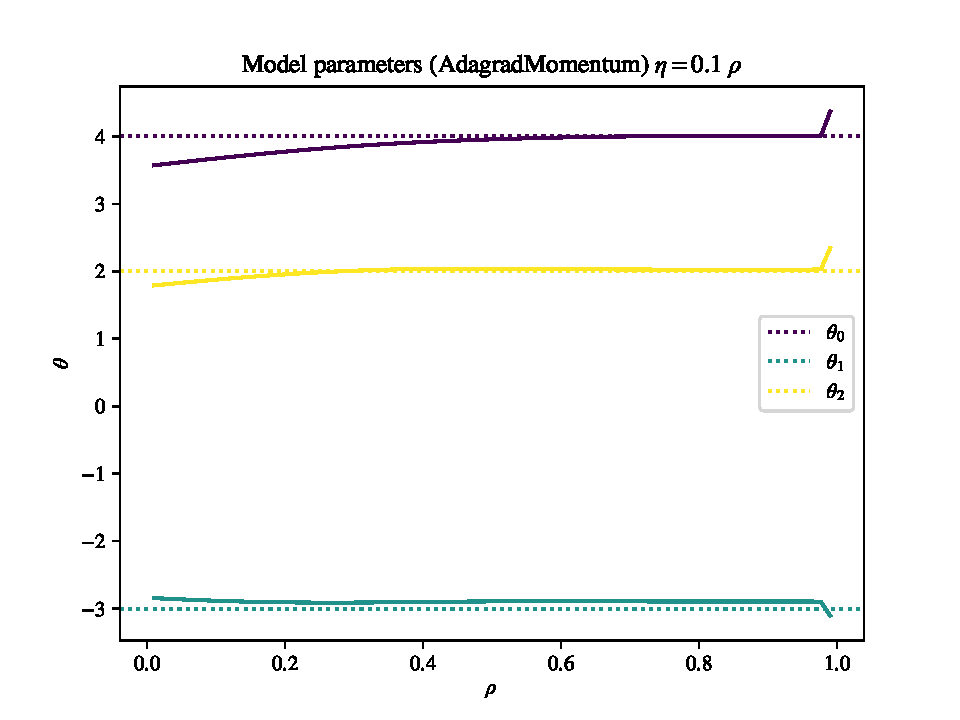
\includegraphics[width=5.5cm]{Project2/figures/polynomial_grad/OLS_autodiff/adagrad_momentum_thetas_rho.pdf} }}%
    \caption{Gradient descent with Adagrad Momentum over 500 epochs with varying $\rho$, $\eta=0.1$.}%
    \label{fig:GDadagradmomentumrho}%
\end{figure}

\begin{figure}[H]%
    \centering
    \subfloat[\centering Heatmap of $\eta$ vs $\rho$.]{{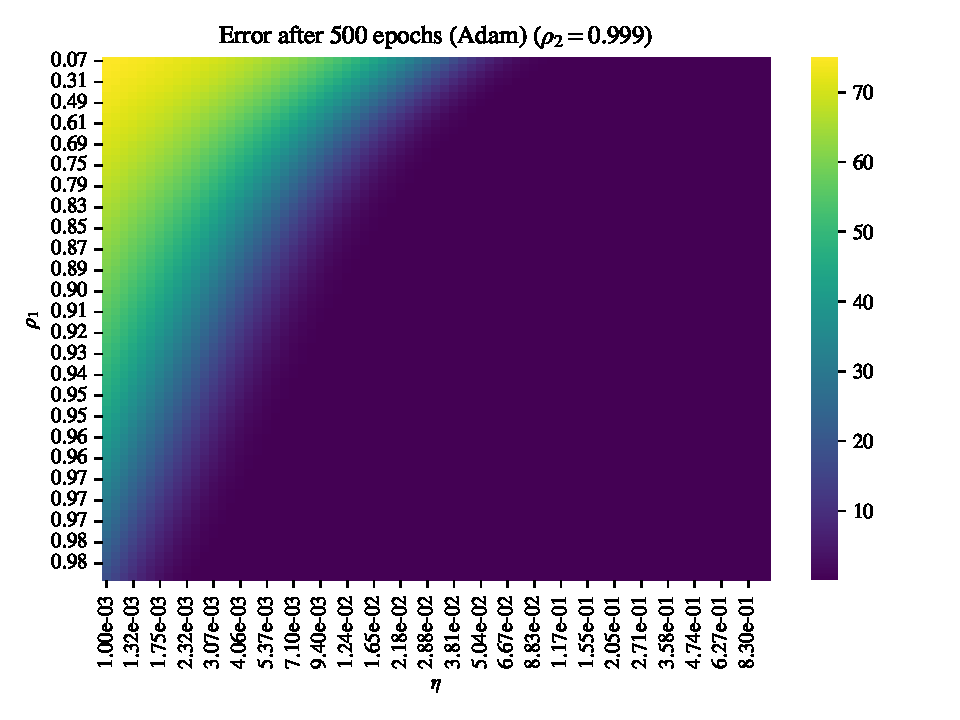
\includegraphics[width=5.5cm]{Project2/figures/polynomial_grad/OLS_autodiff/adagrad_momentum_heatmap_eta_rho.pdf} }}%
    \qquad
    \subfloat[\centering Predicted polynomials for varying $\eta$, $\rho = 0.9$]{{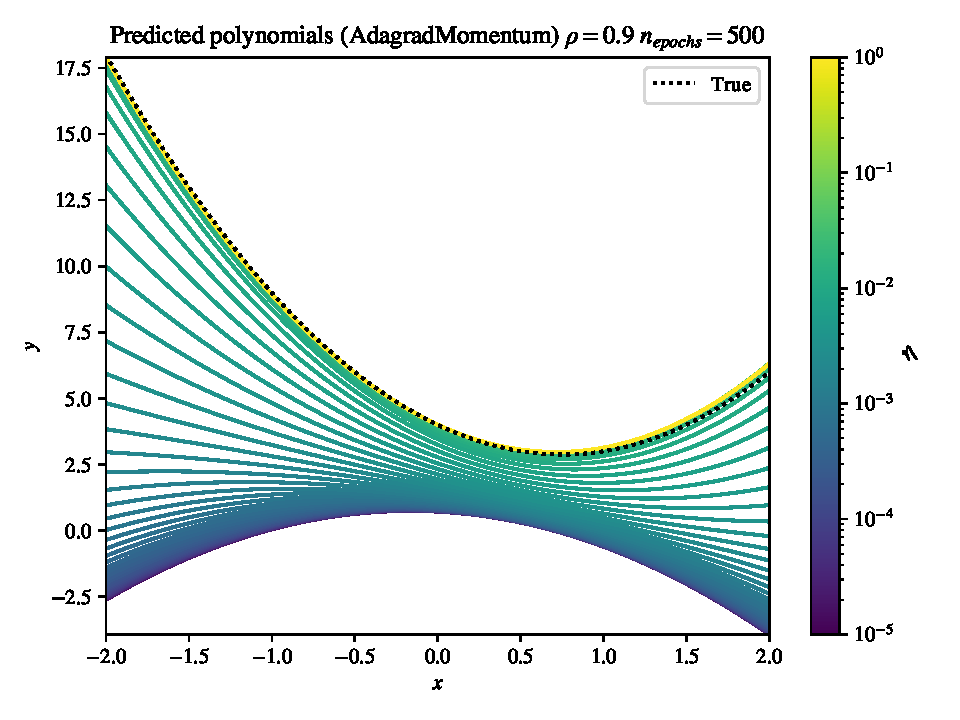
\includegraphics[width=5.5cm]{Project2/figures/polynomial_grad/OLS_autodiff/adagrad_momentum_prediction_eta.pdf} }}%
    \caption{Heatmap and predictions from Gradient descent with Adagrad Momentum over 500 epochs.}%
    \label{fig:GDadagradmomentumheatmappred}%
\end{figure}


\begin{figure}[H]%
    \centering
    \subfloat[\centering Error for varying $\eta$.]{{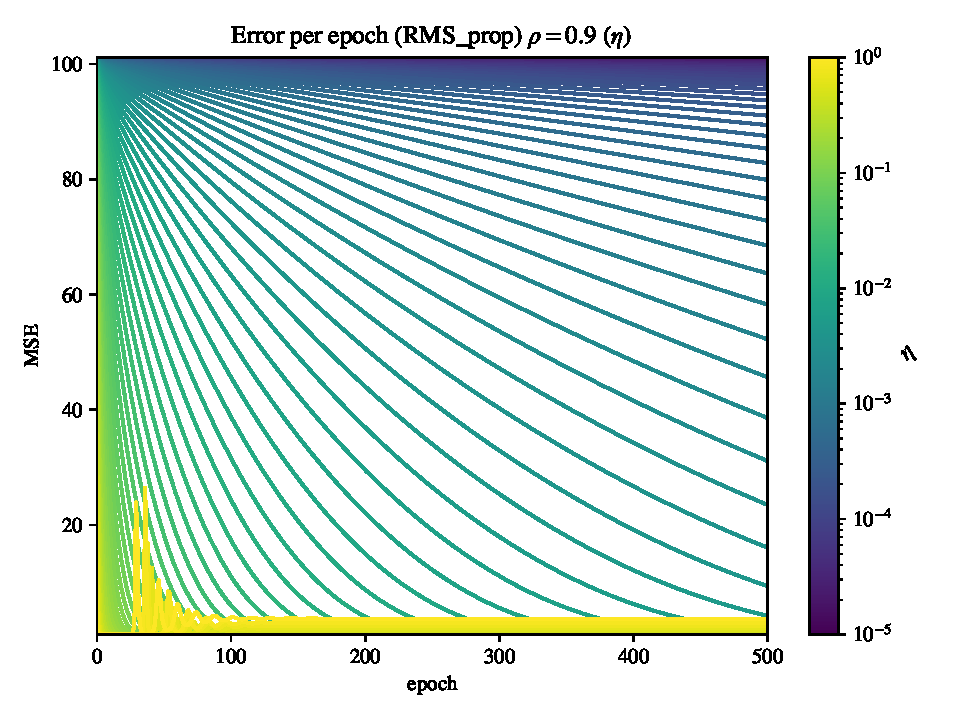
\includegraphics[width=5.5cm]{Project2/figures/polynomial_grad/OLS_autodiff/rms_prop_error_eta.pdf} }}%
    \qquad
    \subfloat[\centering Parameters $\theta$ for varying $\rho$.]{{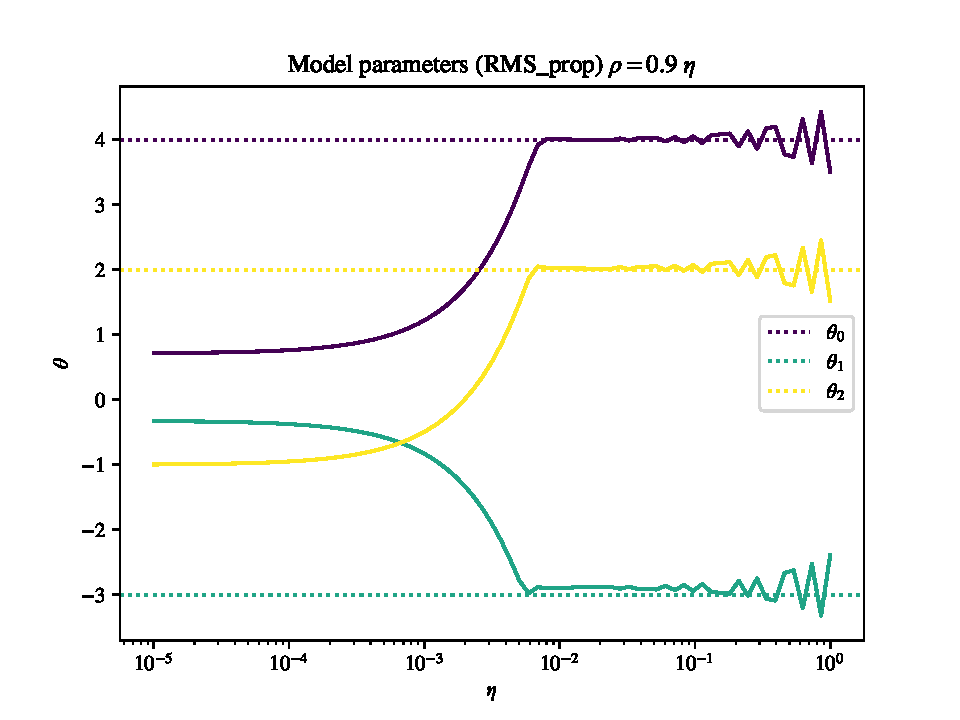
\includegraphics[width=5.5cm]{Project2/figures/polynomial_grad/OLS_autodiff/rms_prop_thetas_eta.pdf} }}%
    \caption{Gradient descent with RMSprop over 500 epochs with varying $\eta$, $\rho=0.9$.}%
    \label{fig:GDrmspropeta}%
\end{figure}

\begin{figure}[H]%
    \centering
    \subfloat[\centering Error for varying $\rho$.]{{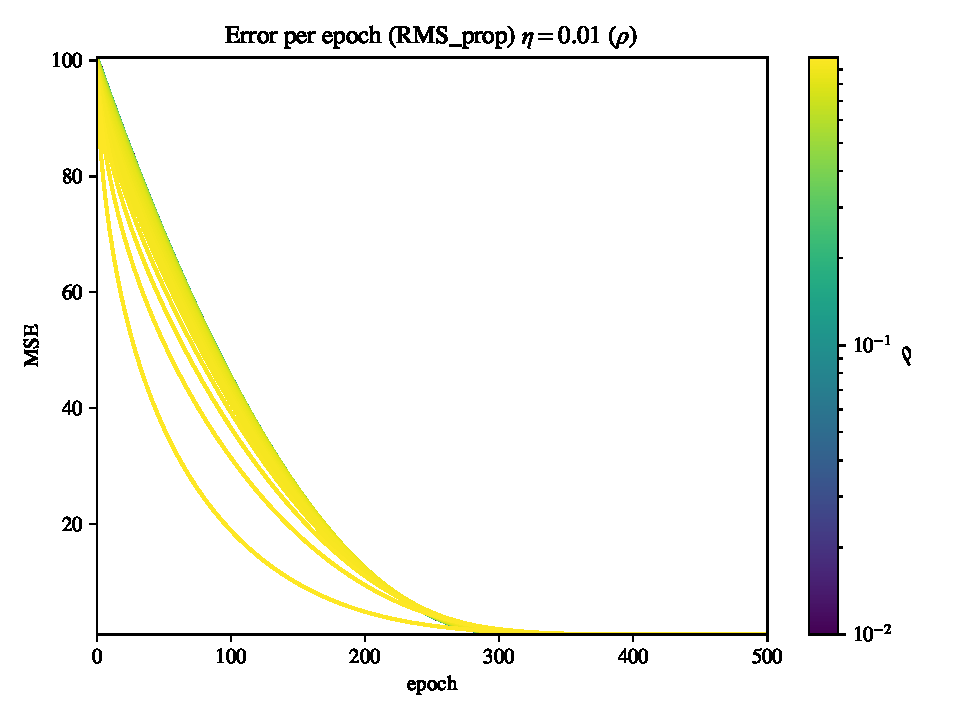
\includegraphics[width=5.5cm]{Project2/figures/polynomial_grad/OLS_autodiff/rms_prop_error_rho.pdf} }}%
    \qquad
    \subfloat[\centering Parameters $\theta$ for varying $\rho$.]{{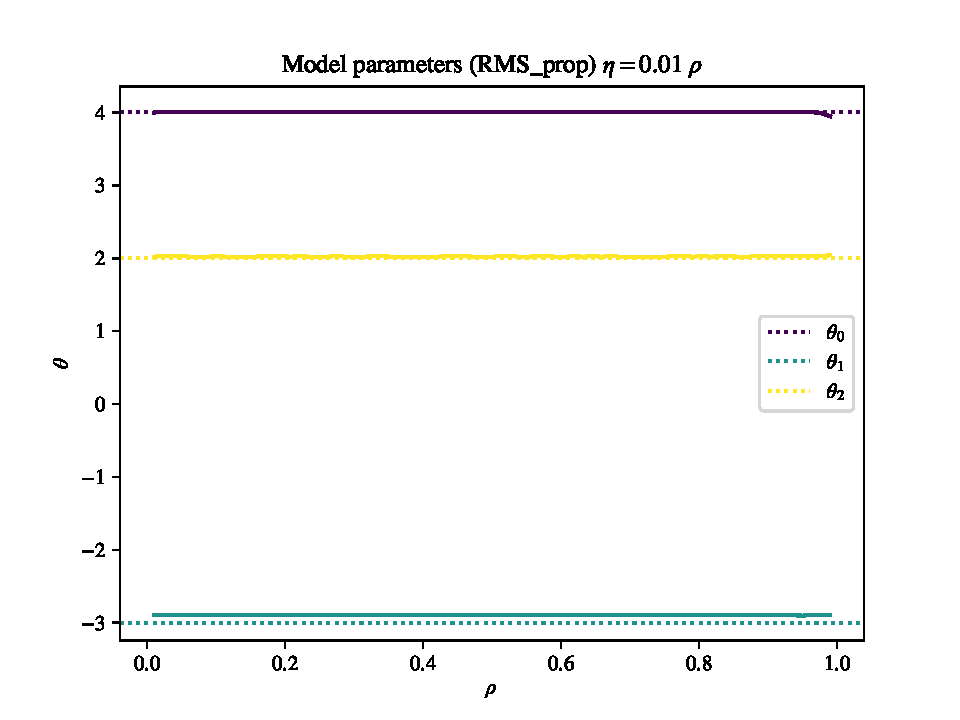
\includegraphics[width=5.5cm]{Project2/figures/polynomial_grad/OLS_autodiff/rms_prop_thetas_rho.pdf} }}%
    \caption{Gradient descent with RMSprop over 500 epochs with varying $\rho$, $\eta=0.01$.}%
    \label{fig:GDrmsproprho}%
\end{figure}

RMSprop gave rather stable results across the varying values of $\rho$, perhaps due to the simple nature of our chosen test function, as seen in \autoref{fig:GDrmsproprho}. The final scheduler applied to deterministic Gradient Descent was Adam, seen in \autoref{fig:GDadameta}. Varying $\rho_1$ in \autoref{fig:GDadamrho1} gave similar results to what we've seen previously. Varying $\rho_2$ in \autoref{fig:GDadamrho2} gave highly chaotic results, and such we will henceforth be sticking with $\rho_2 = 0.999$.

\begin{figure}[H]%
    \centering
    \subfloat[\centering Error for varying $\eta$.]{{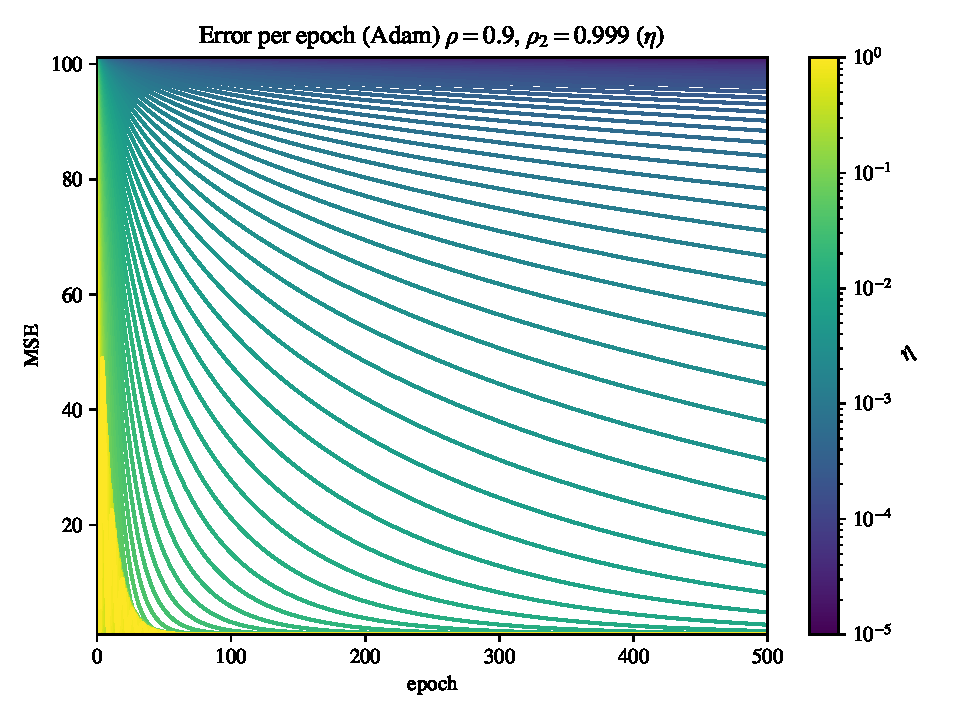
\includegraphics[width=5cm]{Project2/figures/polynomial_grad/OLS_autodiff/adam_error_eta.pdf} }}%
    \qquad
    \subfloat[\centering Parameters $\theta$ for varying $\eta$.]{{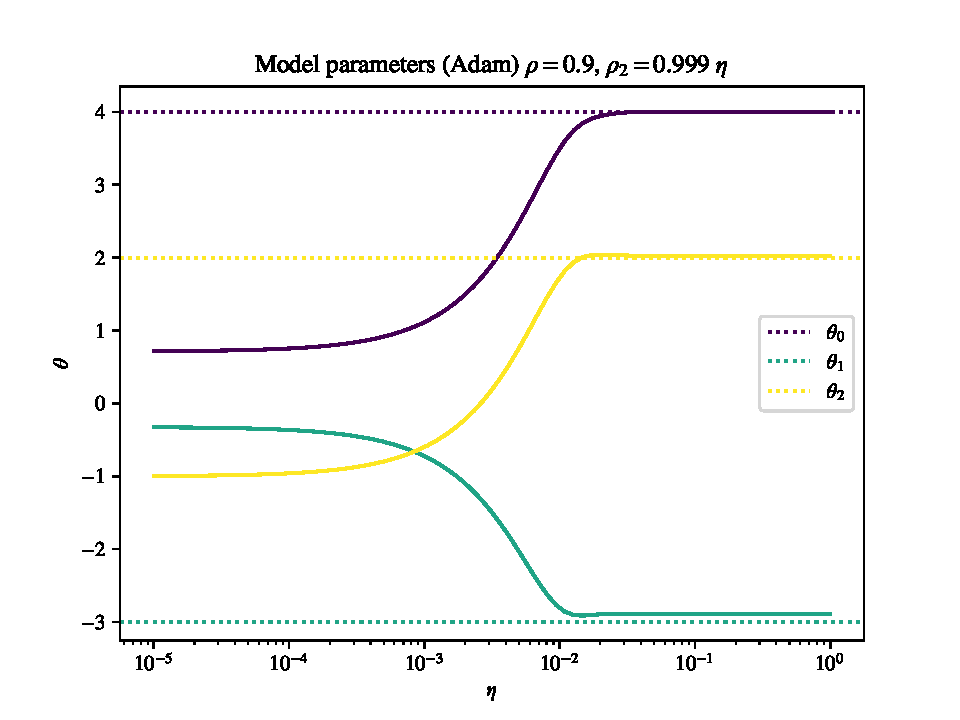
\includegraphics[width=5cm]{Project2/figures/polynomial_grad/OLS_autodiff/adam_thetas_eta.pdf} }}%
    \caption{Gradient descent with Adam over 500 epochs with varying $\eta$, $\rho_1=0.9$ and $\rho_2=0.999$.}%
    \label{fig:GDadameta}%
\end{figure}

\begin{figure}[H]%
    \centering
    \subfloat[\centering Error for varying $\rho_1$.]{{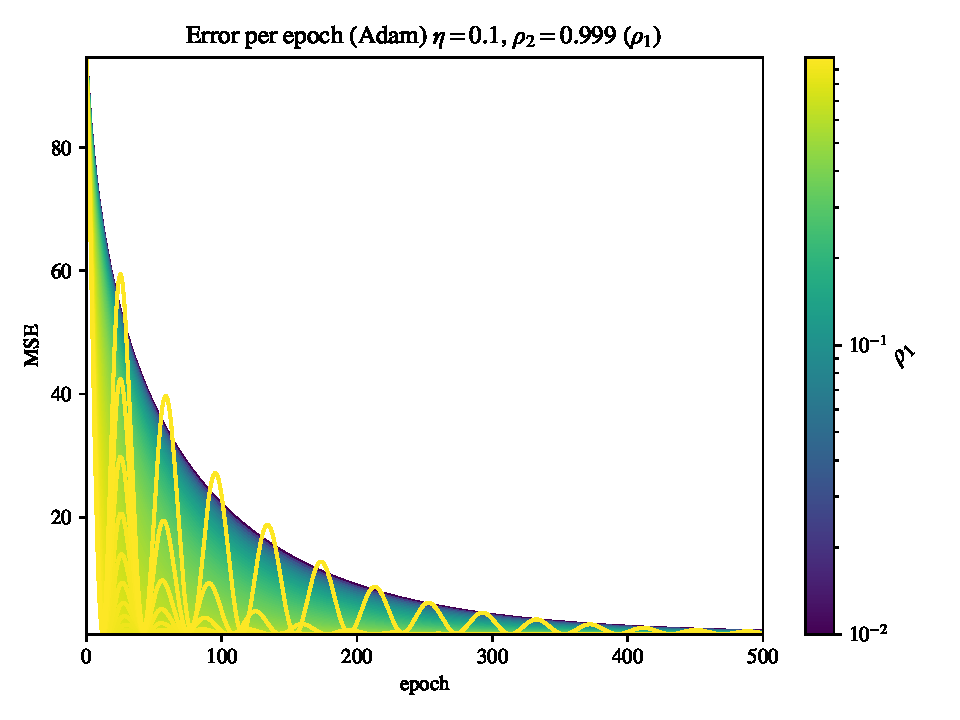
\includegraphics[width=5cm]{Project2/figures/polynomial_grad/OLS_autodiff/adam_error_rho1.pdf} }}%
    \qquad
    \subfloat[\centering Parameters $\theta$ for varying $\rho_1$.]{{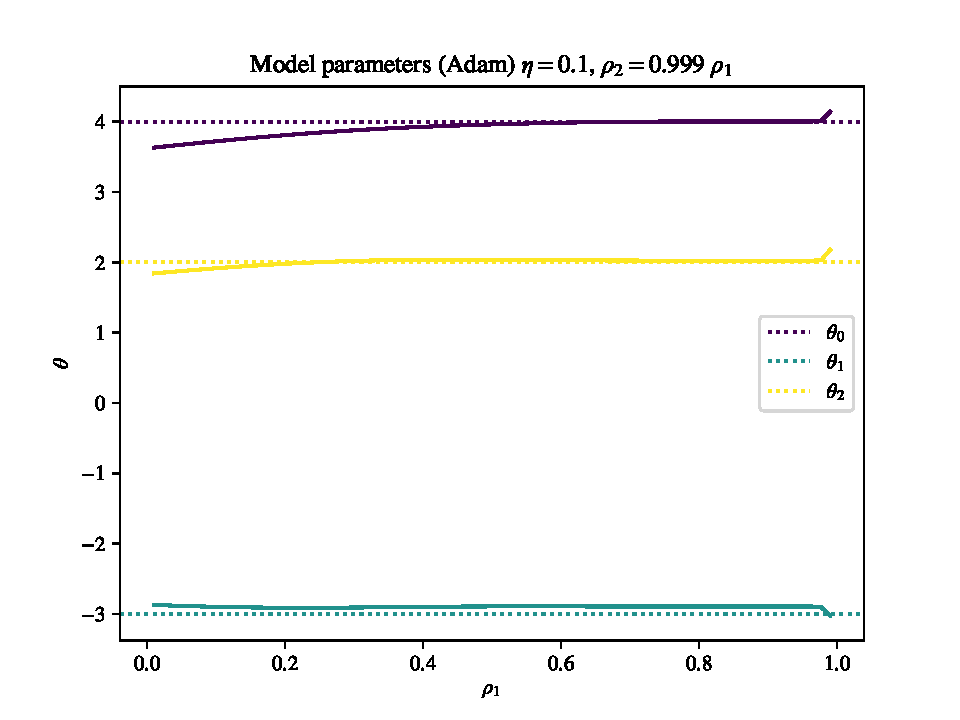
\includegraphics[width=5cm]{Project2/figures/polynomial_grad/OLS_autodiff/adam_thetas_rho1.pdf} }}%
    \caption{Gradient descent with Adam over 500 epochs with varying $\rho_1$, $\eta=0.1$ and $\rho_2=0.999$.}%
    \label{fig:GDadamrho1}%
\end{figure}

\begin{figure}[H]%
    \centering
    \subfloat[\centering Error for varying $\rho_1$.]{{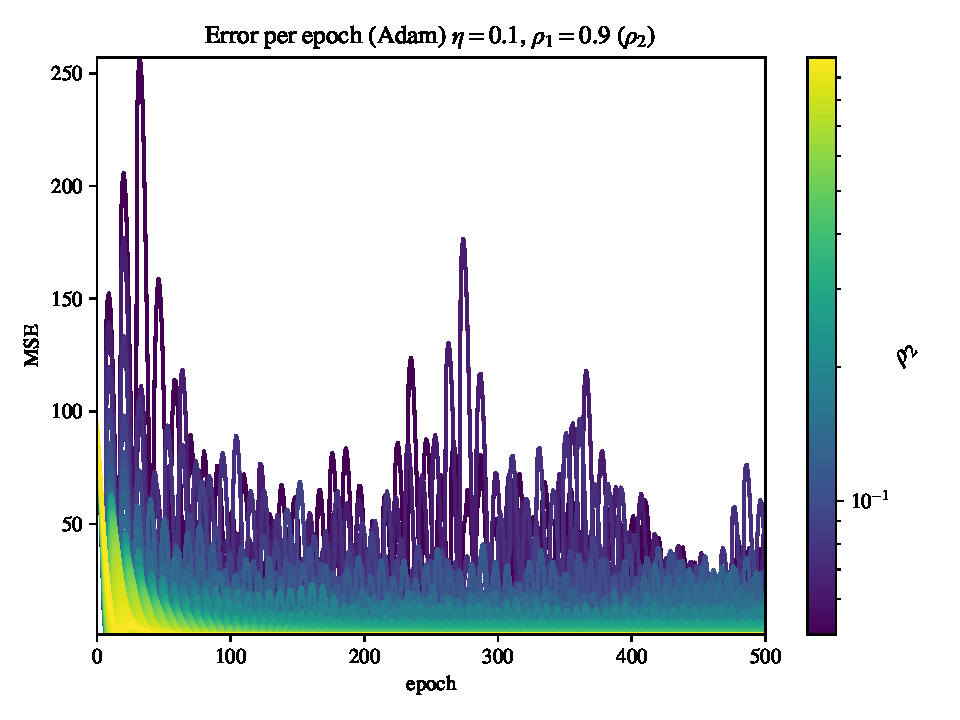
\includegraphics[width=5cm]{Project2/figures/polynomial_grad/OLS_autodiff/adam_error_rho2.pdf} }}%
    \qquad
    \subfloat[\centering Parameters $\theta$ for varying $\rho_2$.]{{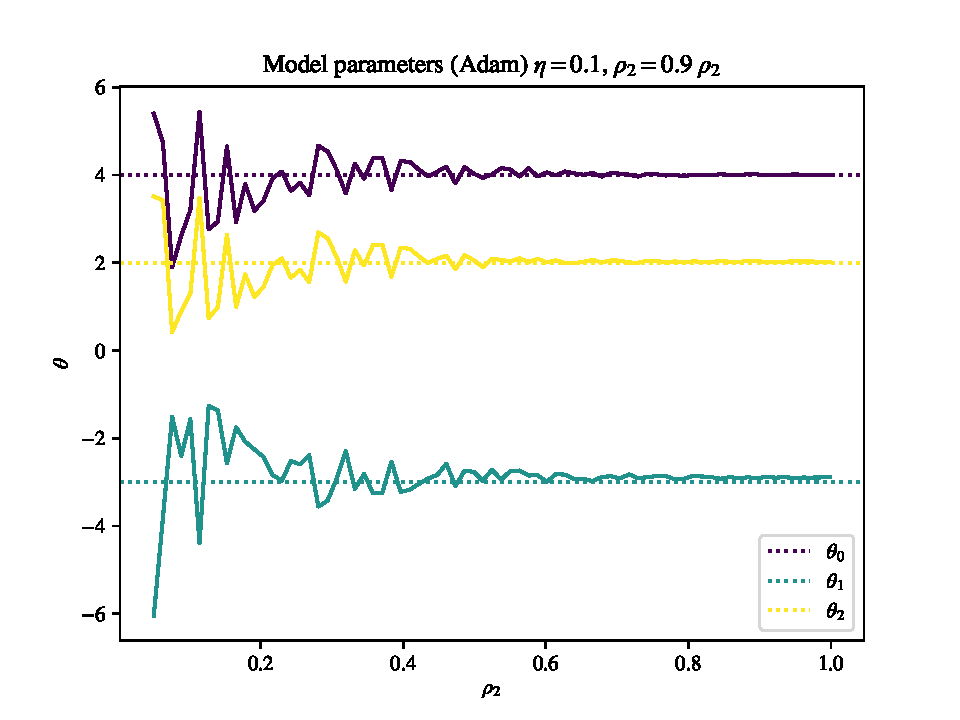
\includegraphics[width=5cm]{Project2/figures/polynomial_grad/OLS_autodiff/adam_thetas_rho2.pdf} }}%
    \caption{Gradient descent with Adam over 500 epochs with varying $\rho_2$, $\eta=0.1$ and $\rho_1=0.9$.}%
    \label{fig:GDadamrho2}%
\end{figure}

\begin{figure}[H]%
    \centering
    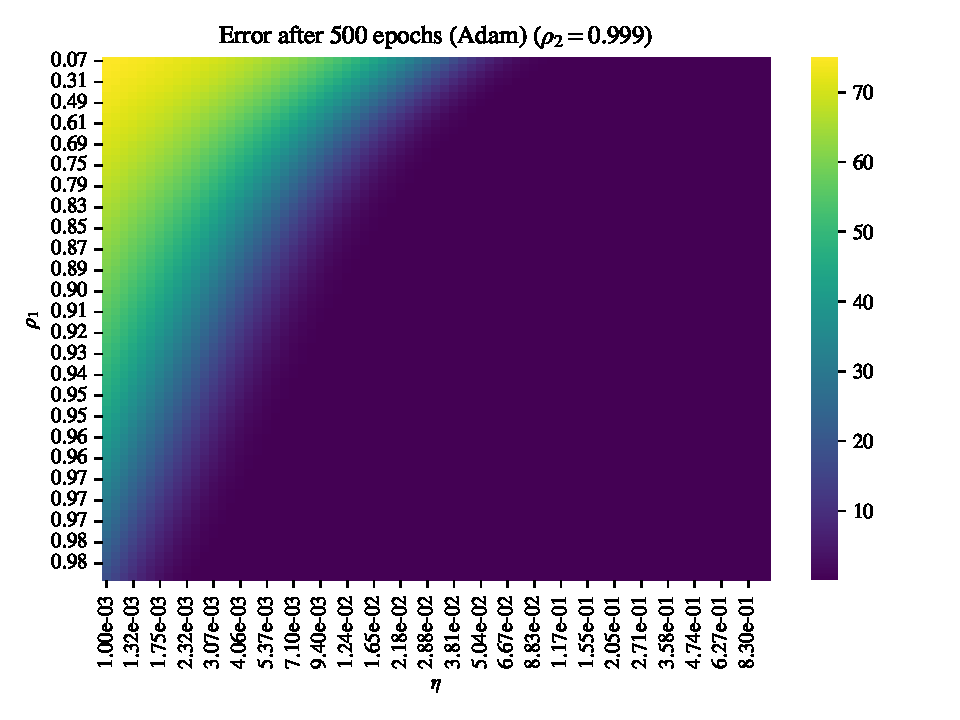
\includegraphics[width=8cm]{Project2/figures/polynomial_grad/OLS_autodiff/adam_momentum_heatmap_eta_rho.pdf}
    \caption{Heatmap of $\rho_1$ vs. $\eta$ for Gradient Descent with Adam after 500 epochs, with $\rho_2 = 0.999$.}
    \label{fig:GDadamheatmap}
\end{figure}

Fixing $\rho_2$ as $0.999$ in \autoref{fig:GDadamheatmap}, we see the equivalent results to what we've seen previously. Notably, a number of these methods were developed for use with Stochastic Gradient Descent, described in \autoref{alg:SGD}.


\begin{figure}[H]%
    \centering
    \subfloat[\centering Error for varying minibatch sizes.]{{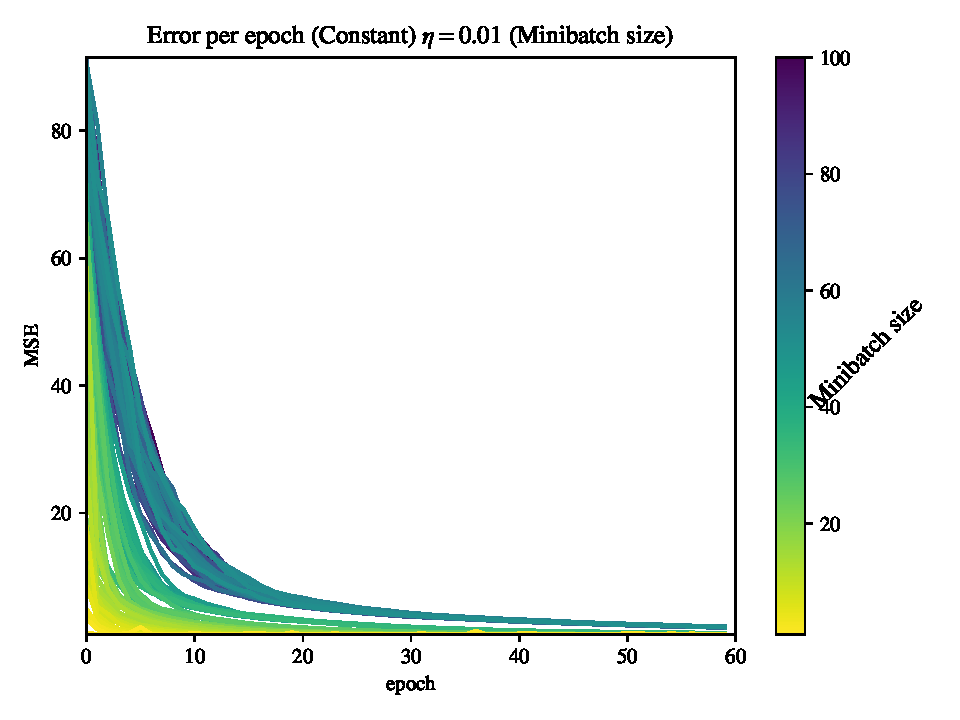
\includegraphics[width=5.5cm]{Project2/figures/polynomial_grad/OLS_analytic/constant_error_minibatch.pdf} }}%
    \qquad
    \subfloat[\centering Parameters $\theta$ for varying minibatch size.]{{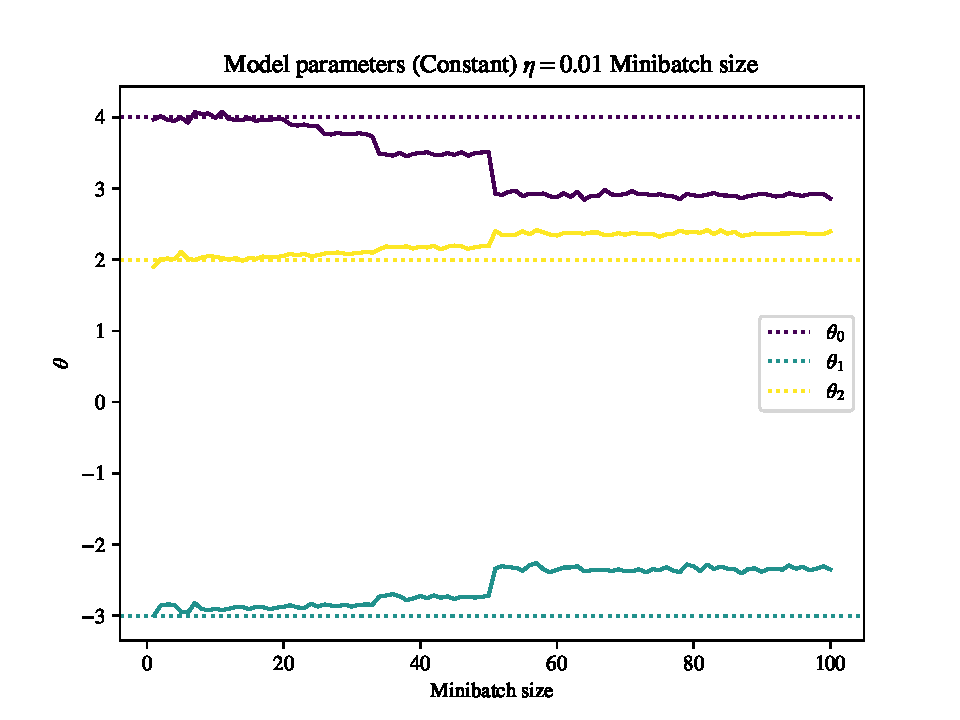
\includegraphics[width=5.5cm]{Project2/figures/polynomial_grad/OLS_analytic/constant_thetas_minibatch.pdf} }}%
    \caption{Stochastic Gradient Descent for varying number of sizes of minibatches over 60 epochs.}%
    \label{fig:SGDconstant}%
\end{figure}

The stochastic noise is evident in \autoref{fig:SGDconstant}. Interestingly, we observe a decrease in accuracy for larger minibatch sizes, perhaps resulting from the sampling of batches being with replacement, as the minibatch size approaches the total number of points 100. % This leads to significant redundancy, particularly when the minibatch size $M$ is close to $100$, the total number of points.

\autoref{alg:SGD} further explains the larger gaps in $(a)$ and the step-like pattern in $(b)$. The number of iterations in its inner loop is determined by $ \left\lfloor\frac{n}{M}\right\rfloor = \left\lfloor\frac{100}{M}\right\rfloor$. This causes abrupt jumps when decreasing the batch size grants the algorithm another iteration, i.e. when $\left\lfloor \frac{100}{M - 1} \right\rfloor = \left\lfloor \frac{100}{M} \right\rfloor + 1$. This is shown more clearly in \autoref{fig:SGDadagrad}.

\begin{figure}[H]%
    \centering
    \subfloat[\centering Error for varying minibatch sizes]{{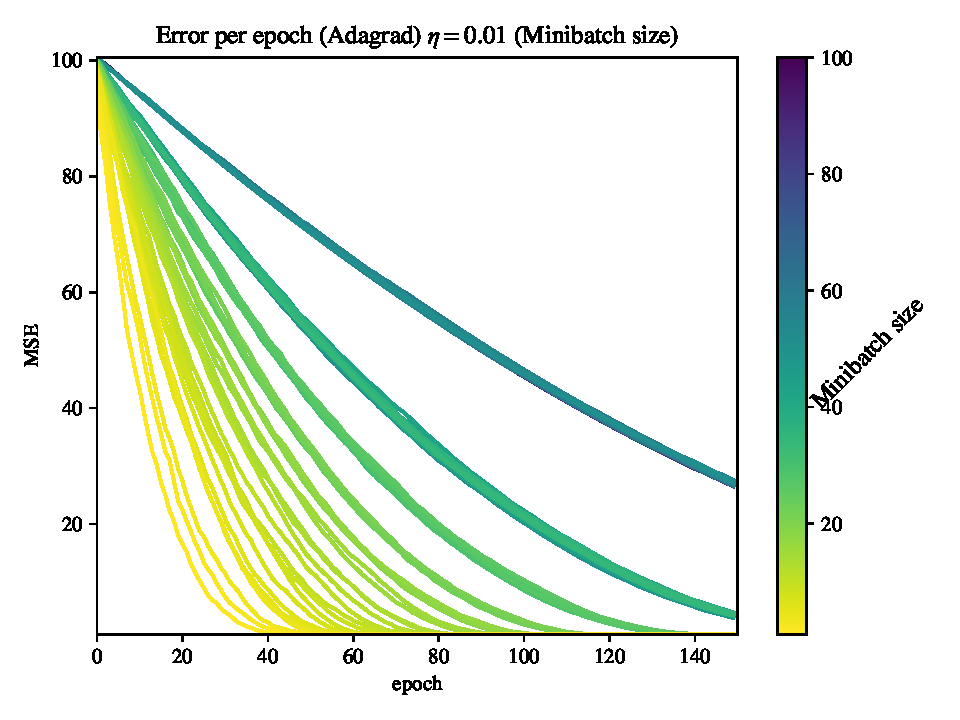
\includegraphics[width=5.5cm]{Project2/figures/polynomial_grad/OLS_autodiff/adagrad_error_minibatch.pdf} }}%
    \qquad
    \subfloat[\centering Parameters $\theta$ for batchsize]{{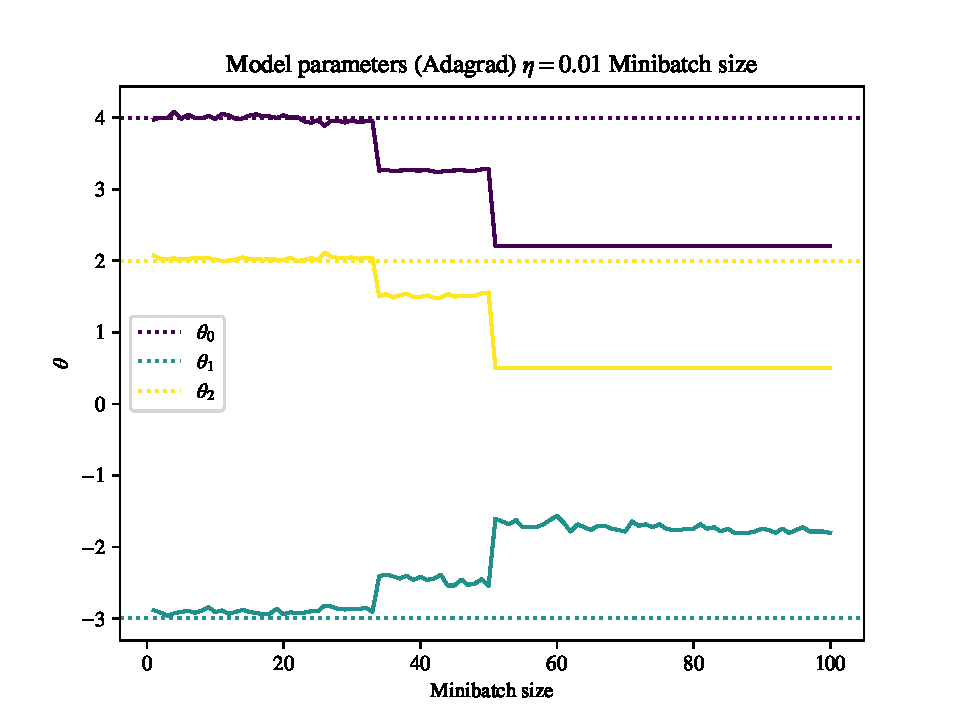
\includegraphics[width=5.5cm]{Project2/figures/polynomial_grad/OLS_autodiff/adagrad_thetas_minibatch.pdf} }}%
    \caption{Stochastic Gradient Descent with Adagrad over 150 epochs with $\eta = 0.1$}%
    \label{fig:SGDadagrad}%
\end{figure}

These gaps are again different for ADAM in \autoref{fig:SGDadam}.
These differences stem from the resetting of the cumulative memory parameters for each 
epoch. Remember from
\autoref{AdamAmp} how the amplification of step size is largest at the beginning of the iteration. This causes the steeper steps in \autoref{fig:SGDadam} (b), greatly affecting the convergence rate seen in \autoref{fig:SGDadamerror}

\begin{figure}[H]%
    \centering
    \subfloat[\centering Error for varying minibatch sizes]{{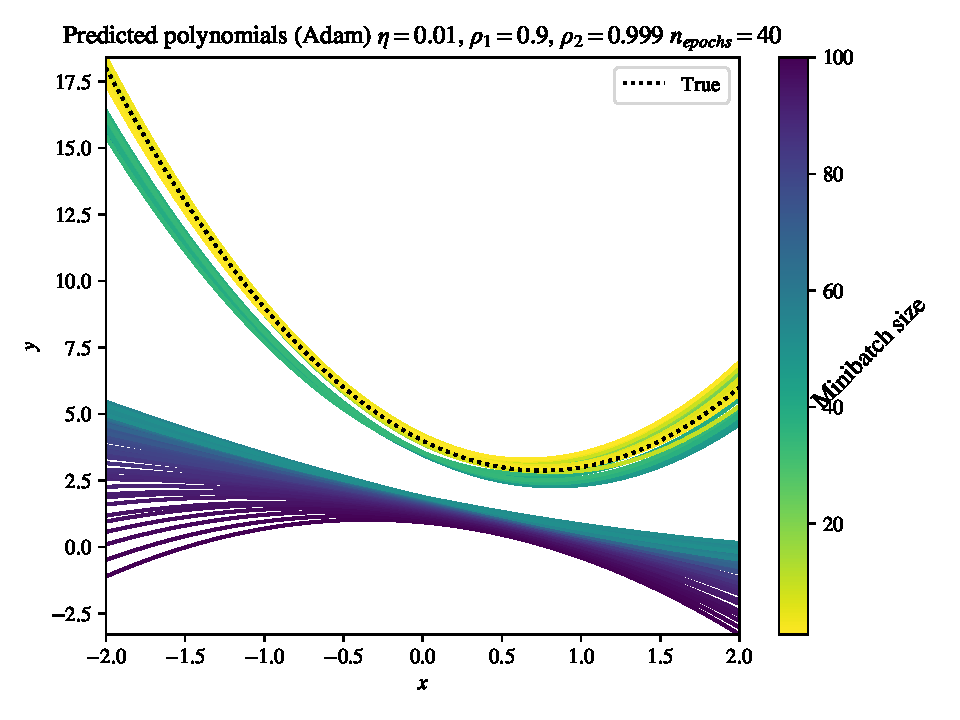
\includegraphics[width=5.5cm]{Project2/figures/polynomial_grad/OLS_autodiff/adam_prediction_minibatch.pdf} }}%
    \qquad
    \subfloat[\centering Parameters $\theta$ for batchsize]{{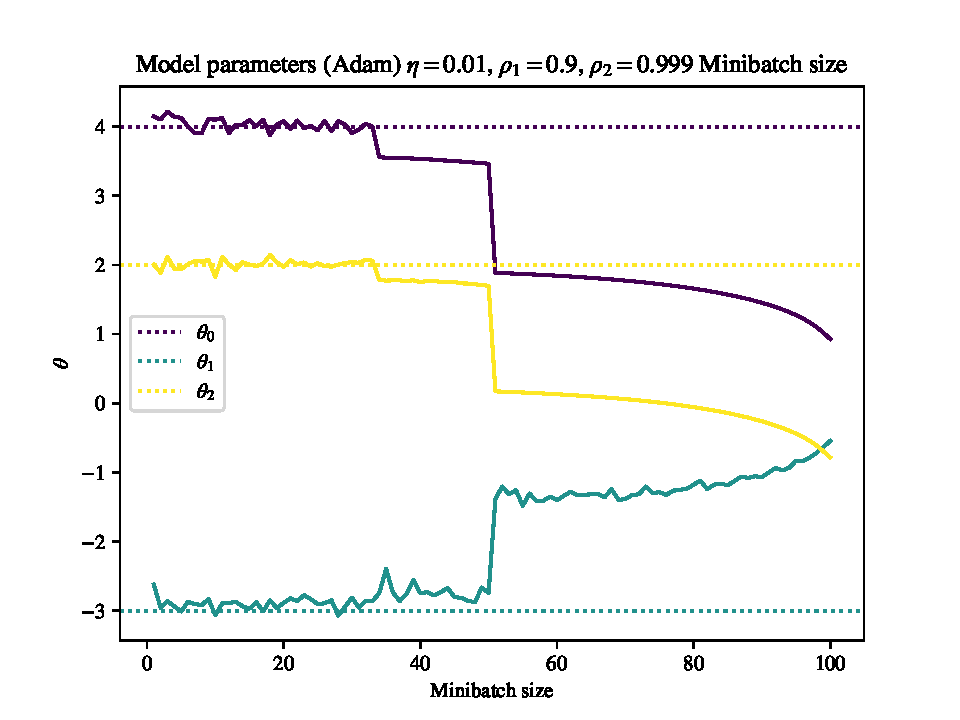
\includegraphics[width=5.5cm]{Project2/figures/polynomial_grad/OLS_autodiff/adam_thetas_minibatch.pdf} }}%
    \caption{Stochastic Gradient Descent with Adam over 40 epochs with $\rho_2$ = 0.999, $\rho_1=0.9$ and $\eta = 0.01$}%
    \label{fig:SGDadam}%
\end{figure}

\begin{figure}[H]%
    \centering
    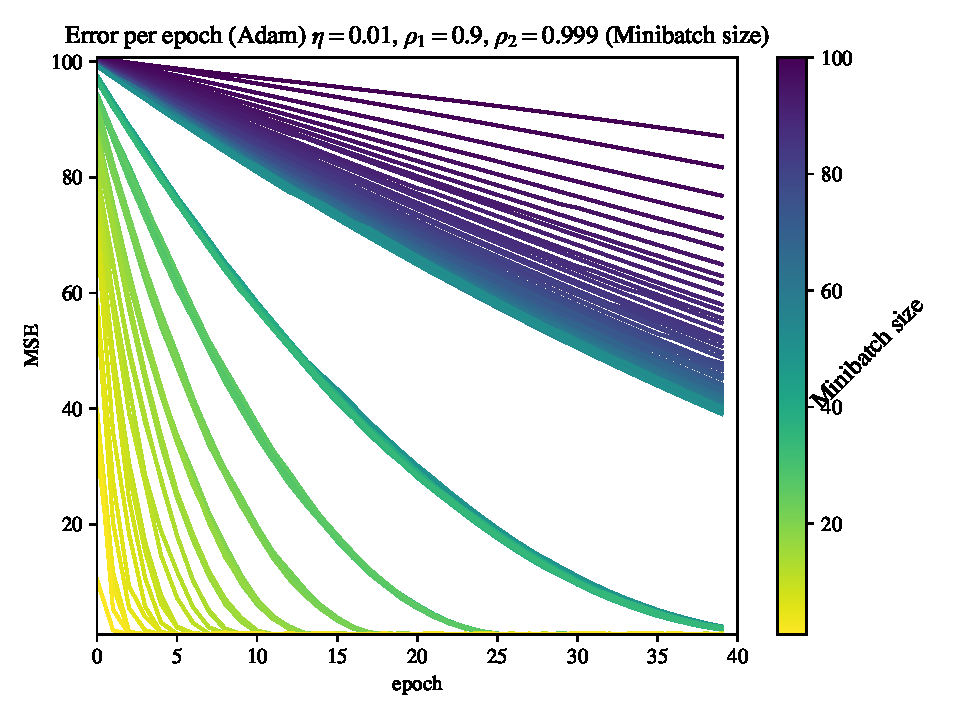
\includegraphics[width=8cm]{Project2/figures/polynomial_grad/OLS_autodiff/adam_error_minibatch.pdf}
    \caption{Error for Stochastic Gradient Descent with Adam after 40 epochs, with $\rho_2 = 0.999$ and $\eta=0.01$.}
    \label{fig:SGDadamerror}
\end{figure}

\begin{figure}[H]%
    \centering
    \subfloat[\centering Error for varying minibatch sizes]{{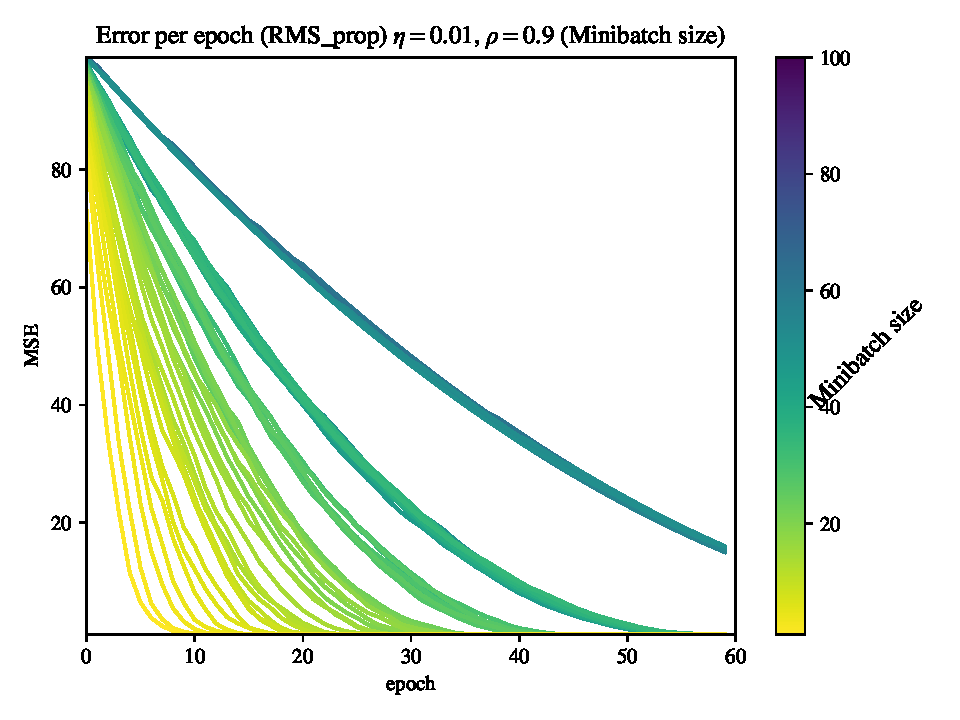
\includegraphics[width=5.5cm]{Project2/figures/polynomial_grad/OLS_autodiff/rms_prop_error_minibatch.pdf} }}%
    \qquad
    \subfloat[\centering Parameters $\theta$ for batchsize]{{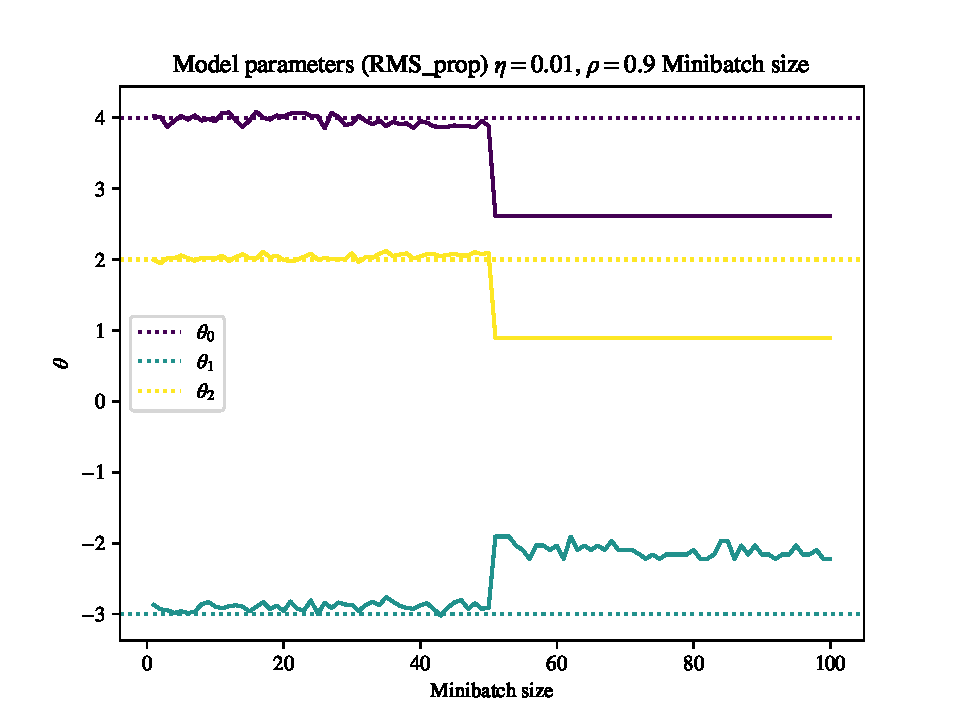
\includegraphics[width=5.5cm]{Project2/figures/polynomial_grad/OLS_autodiff/rms_prop_thetas_minibatch.pdf} }}%
    \caption{Stochastic Gradient Descent with RMSprop over 60 epochs with $\rho = 0.9$ and $\eta = 0.1$}%
    \label{fig:SGDrmsprop}%
\end{figure}

With RMSprop we see the steepest steps, approximately converging with just two batches as seen in \autoref{fig:SGDrmsprop}. We see interesting behaviour with time decay in \autoref{fig:SGDtimedecay}, starting out with rapid convergence, but quickly stabilizing at various degrees of success. This is not suprising, giving the simplistic nature of the scheduler. It has less significant jumps, being also dependent on the size of the batches.

\begin{figure}[H]%
    \centering
    \subfloat[\centering Error for varying minibatch sizes]{{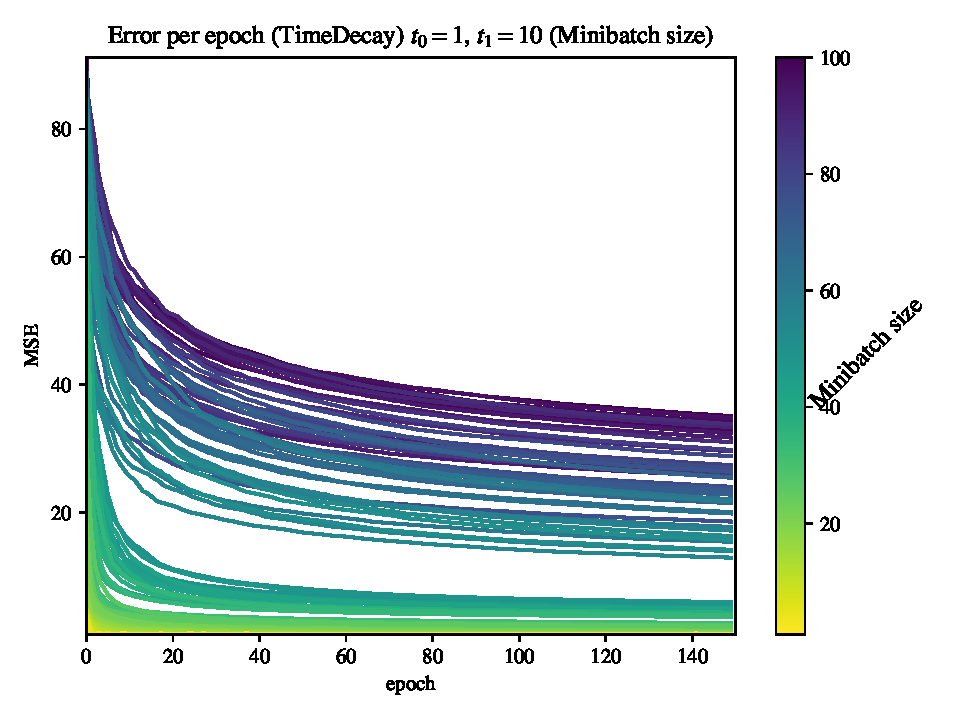
\includegraphics[width=5.5cm]{Project2/figures/polynomial_grad/OLS_autodiff/time_decay_error_minibatch.pdf} }}%
    \qquad
    \subfloat[\centering Parameters $\theta$ for batchsize]{{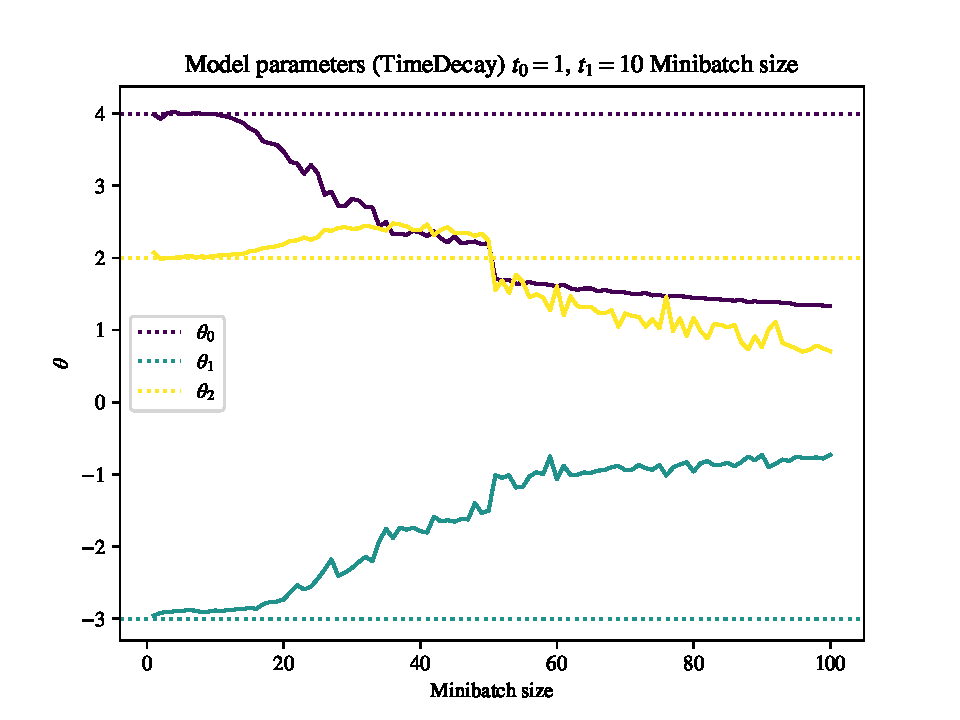
\includegraphics[width=5.5cm]{Project2/figures/polynomial_grad/OLS_autodiff/time_decay_thetas_minibatch.pdf} }}%
    \caption{Stochastic Gradient Descent with Time decay over 150 epochs with $t_0 = 1$ and $t_1 = 10$}%
    \label{fig:SGDtimedecay}%
\end{figure}

Perhaps the most interesting graph, is seen in \autoref{fig:SGDadagradmomentum} with Momentum and Adagrad Momentum. Here we can clearly see the similarities between the approaches. Note that while the standard Momentum approach converges faster, it jumps up for a bit after first bottoming out, a behaviour we hardly see with Adagrad.

\begin{figure}[H]%
    \centering
    \subfloat[\centering Adagrad Momentum]{{\includegraphics[width=5.5cm]{Project2/figures/polynomial_grad/OLS_autodiff/adagrad_momentum_error_minibatch.pdf} }}%
    \qquad
    \subfloat[\centering Momentum]{{\includegraphics[width=5.5cm]{Project2/figures/polynomial_grad/OLS_autodiff/momentum_error_minibatch.pdf} }}%
    \caption{Error for varying size of minibatches from Stochastic Gradient Descent with Momentum and Adagrad Momentum over 60 epochs with $\eta = 0.01$ and $\rho = 0.9$}%
    \label{fig:SGDadagradmomentum}%
\end{figure}

\newpage
\subsection{Franke's function}
With a better understanding of how drastic our choices of hyperparameters can affect our final results, we begin by exploring Franke's function through the use of a neural network. There are a lot of moving parts, with varying learning rates, regularization terms, activation function, etc. In order to get any results, we fix the hyperparameters for the schedulers from what has previously been shown to work, namely $\rho/\rho_1 = 0.9$, $\rho_2 = 0.999$. We also restrict ourselves to 100 epochs with a minibatch size of 40. For the sake of consistency, the neural networks all consisted of three hidden layers of width respectively 75, 75 and 100. Due to computational constraints, we only applied a $80 / 20$ train-validation split to see how well the networks perform on unseen data.

Note that due to a typo, the $y$-axis of the heatmaps are labeled $\rho$ when they should be $\lambda$. What follows are heatmaps of the final validation error for varying combinations of scheduler and hidden function, plotted in $\log$-scale.
\begin{figure}[H]%
    \centering
    \subfloat[\centering Sigmoid]{{\includegraphics[width=5.5cm]{Project2/figures/franke/constant/sigmoid_validation_error_heatmap.pdf} }}%
    \qquad
    \subfloat[\centering (0,1)-clip]{{\includegraphics[width=5.5cm]{Project2/figures/franke/constant/zero_one_clip_validation_error_heatmap.pdf} }}%
    \caption{Heatmap of $\eta$ vs. $\lambda$ for constant scheduler}%
    \label{fig:FrankeConstant}%
\end{figure}

\begin{figure}[H]%
    \centering
    \subfloat[\centering Sigmoid]{{\includegraphics[width=5.5cm]{Project2/figures/franke/momentum/sigmoid_validation_error_heatmap.pdf} }}%
    \qquad
    \subfloat[\centering (0,1)-clip]{{\includegraphics[width=5.5cm]{Project2/figures/franke/momentum/zero_one_clip_validation_error_heatmap.pdf} }}%
    \caption{Heatmap of $\eta$ vs. $\lambda$ for momentum scheduler}%
    \label{fig:FrankeMomentum}%
\end{figure}

\begin{figure}[H]%
    \centering
    \subfloat[\centering Sigmoid]{{\includegraphics[width=5.5cm]{Project2/figures/franke/adagrad/sigmoid_validation_error_heatmap.pdf} }}%
    \qquad
    \subfloat[\centering (0,1)-clip]{{\includegraphics[width=5.5cm]{Project2/figures/franke/adagrad/zero_one_clip_validation_error_heatmap.pdf} }}%
    \\% 
    \subfloat[\centering ReLU]{{\includegraphics[width=5.5cm]{Project2/figures/franke/adagrad/relu_validation_error_heatmap.pdf} }}%
    \qquad
    \subfloat[\centering LReLU]{{\includegraphics[width=5.5cm]{Project2/figures/franke/adagrad/lrelu_validation_error_heatmap.pdf} }}%
    \caption{Heatmap of $\eta$ vs. $\lambda$ for Adagrad scheduler}%
    \label{fig:FrankeAdagrad}%
\end{figure}


\begin{figure}[H]%
    \centering
    \subfloat[\centering Sigmoid]{{\includegraphics[width=5.5cm]{Project2/figures/franke/adagradmomentum/sigmoid_validation_error_heatmap.pdf} }}%
    \qquad
    \subfloat[\centering (0,1)-clip]{{\includegraphics[width=5.5cm]{Project2/figures/franke/adagradmomentum/zero_one_clip_validation_error_heatmap.pdf} }}%
    \\% 
    \subfloat[\centering ReLU]{{\includegraphics[width=5.5cm]{Project2/figures/franke/adagradmomentum/relu_validation_error_heatmap.pdf} }}%
    \qquad
    \subfloat[\centering LReLU]{{\includegraphics[width=5.5cm]{Project2/figures/franke/adagradmomentum/lrelu_validation_error_heatmap.pdf} }}%
    \caption{Heatmap of $\eta$ vs. $\lambda$ for AdagradMomentum scheduler}%
    \label{fig:FrankeAdagradMomentum}%
\end{figure}

\begin{figure}[H]%
    \centering
    \subfloat[\centering Sigmoid]{{\includegraphics[width=5.5cm]{Project2/figures/franke/rms_prop/sigmoid_validation_error_heatmap.pdf} }}%
    \qquad
    \subfloat[\centering (0,1)-clip]{{\includegraphics[width=5.5cm]{Project2/figures/franke/rms_prop/zero_one_clip_validation_error_heatmap.pdf} }}%
    \\% 
    \subfloat[\centering ReLU]{{\includegraphics[width=5.5cm]{Project2/figures/franke/rms_prop/relu_validation_error_heatmap.pdf} }}%
    \qquad
    \subfloat[\centering LReLU]{{\includegraphics[width=5.5cm]{Project2/figures/franke/rms_prop/lrelu_validation_error_heatmap.pdf} }}%
    \caption{Heatmap of $\eta$ vs. $\lambda$ for RMSprop scheduler}%
    \label{fig:FrankeRMSprop}%
\end{figure}

\begin{figure}[H]%
    \centering
    \subfloat[\centering Sigmoid]{{\includegraphics[width=5.5cm]{Project2/figures/franke/adam/sigmoid_validation_error_heatmap.pdf} }}%
    \qquad
    \subfloat[\centering (0,1)-clip]{{\includegraphics[width=5.5cm]{Project2/figures/franke/adam/zero_one_clip_validation_error_heatmap.pdf} }}%
    \\% 
    \subfloat[\centering ReLU]{{\includegraphics[width=5.5cm]{Project2/figures/franke/adam/relu_validation_error_heatmap.pdf} }}%
    \qquad
    \subfloat[\centering LReLU]{{\includegraphics[width=5.5cm]{Project2/figures/franke/adam/lrelu_validation_error_heatmap.pdf} }}%
    \caption{Heatmap of $\eta$ vs. $\lambda$ for Adam scheduler}%
    \label{fig:FrankeAdam}%
\end{figure}

Selecting the top performers from each, we get

\begin{figure}[H]%
    \centering
    \subfloat[\centering Sigmoid]{{\includegraphics[width=8.5cm]{Project2/figures/franke/constant/constant_sigmoid_surface.pdf} }}%
    \\
    \subfloat[\centering (0,1)-clip]{{\includegraphics[width=8.5cm]{Project2/figures/franke/constant/constant_zero_one_clip_surface.pdf} }}%
    \caption{Predicted surface and absolute error with constant scheduler.}%
    \label{fig:FrankeConstantsurf}%
\end{figure}

In \autoref{fig:FrankeConstantsurf} we see drastically different surfaces visually, however they had comparable validation error as seen in \autoref{fig:FrankeConstant}. 

\begin{figure}[H]%
    \centering
    \subfloat[\centering Sigmoid]{{\includegraphics[width=8.5cm]{Project2/figures/franke/momentum/momentum_sigmoid_surface.pdf} }}%
    \\
    \subfloat[\centering (0,1)-clip]{{\includegraphics[width=8.5cm]{Project2/figures/franke/momentum/momentum_zero_one_clip_surface.pdf} }}%
    \caption{Predicted surface and absolute error with momentum scheduler.}%
    \label{fig:FrankeMomentumsurf}%
\end{figure}

Selecting the top performers from \autoref{fig:FrankeMomentum} generated \autoref{fig:FrankeMomentumsurf}. Note that (b) supposedly had better results, which might be due to it having slimmer ``peaks'', rather than (a)'s more continuous errors.

\begin{figure}[H]%
    \centering
    \subfloat[\centering Adam]{{\includegraphics[width=8.5cm]{Project2/figures/franke/adam/adam_ReLU_surface.pdf} }}%
    \\
    \subfloat[\centering Adagrad]{{\includegraphics[width=8.5cm]{Project2/figures/franke/adagrad/adagrad_ReLU_surface.pdf} }}%
    \caption{Predicted surfaces using ReLU, with Adam and Adagrad.}%
    \label{fig:FrankeReLU}%
\end{figure}

We had wildly inconsistent results using ReLU and LReLU, illustrated in \autoref{fig:FrankeReLU}, the reason for this is at the time of writing unknown to the authors.

\begin{figure}[H]%
    \centering
    \subfloat[\centering Adam with sigmoid]{{\includegraphics[width=8.5cm]{Project2/figures/franke/adam/adam_sigmoid_surface.pdf} }}%
    \\
    \subfloat[\centering AdagradMomentum with (0,1)-clip]{{\includegraphics[width=8.5cm]{Project2/figures/franke/adagradmomentum/adagradmomentum_zero_one_clip_surface.pdf} }}%
    \caption{Top performing predictions of Franke's function.}%
    \label{fig:FrankeBest}%
\end{figure}

Our top performers were found with the combination of the Adam scheduler and sigmoid activation functions, and Adagrad Momentum with (0,1)-clip, illustrated in \autoref{fig:FrankeBest}. Keep in mind that these results were generated with a comparatively small neural network, run over a limited number of iterations.

\newpage
\subsection{Tumor classification}
When exploring the optimal parameters, we ran into the same issues with ReLU and LReLU as seen previously, illustrated here in \autoref{fig:cancerRelu}. They are therefore excluded from this section.
\begin{figure}[H]
    \centering
    \includegraphics[width=8cm]{Project2/figures/cancer_classification/ReLU_Adam_accuracy.pdf}
    \caption{Accuracy when using ReLU as the hidden activation function.}
    \label{fig:cancerRelu}
\end{figure}

\begin{figure}[H]%
    \centering
    \subfloat[\centering Sigmoid]{{\includegraphics[width=5.5cm]{Project2/figures/cancer_classification/sigmoid_Constant_accuracy.pdf} }}%
    \qquad
    \subfloat[\centering (0,1)-clip]{{\includegraphics[width=5.5cm]{Project2/figures/cancer_classification/zero_one_clip_Constant_accuracy.pdf} }}%
    \caption{Heatmap of $\eta$ vs. $\lambda$ for constant scheduler.}%
    \label{fig:CancerConstant}%
\end{figure}

\begin{figure}[H]%
    \centering
    \subfloat[\centering Sigmoid]{{\includegraphics[width=5.5cm]{Project2/figures/cancer_classification/sigmoid_Momentum_accuracy.pdf} }}%
    \qquad
    \subfloat[\centering (0,1)-clip]{{\includegraphics[width=5.5cm]{Project2/figures/cancer_classification/zero_one_clip_Momentum_accuracy.pdf} }}%
    \caption{Heatmap of $\eta$ vs. $\lambda$ for Momentum scheduler.}%
    \label{fig:CancerMomentum}%
\end{figure}

\begin{figure}[H]%
    \centering
    \subfloat[\centering Sigmoid]{{\includegraphics[width=5.5cm]{Project2/figures/cancer_classification/sigmoid_Adagrad_accuracy.pdf} }}%
    \qquad
    \subfloat[\centering (0,1)-clip]{{\includegraphics[width=5.5cm]{Project2/figures/cancer_classification/zero_one_clip_Adagrad_accuracy.pdf} }}%
    \caption{Heatmap of $\eta$ vs. $\lambda$ for Adagrad scheduler.}%
    \label{fig:CancerAdagrad}%
\end{figure}

\begin{figure}[H]%
    \centering
    \subfloat[\centering Sigmoid]{{\includegraphics[width=5.5cm]{Project2/figures/cancer_classification/sigmoid_AdagradMomentum_accuracy.pdf} }}%
    \qquad
    \subfloat[\centering (0,1)-clip]{{\includegraphics[width=5.5cm]{Project2/figures/cancer_classification/zero_one_clip_AdagradMomentum_accuracy.pdf} }}%
    \caption{Heatmap of $\eta$ vs. $\lambda$ for AdagradMomentum scheduler.}%
    \label{fig:CancerAdagradMomentum}%
\end{figure}

\begin{figure}[H]%
    \centering
    \subfloat[\centering Sigmoid]{{\includegraphics[width=5.5cm]{Project2/figures/cancer_classification/sigmoid_Adam_accuracy.pdf} }}%
    \qquad
    \subfloat[\centering (0,1)-clip]{{\includegraphics[width=5.5cm]{Project2/figures/cancer_classification/zero_one_clip_Adam_accuracy.pdf} }}%
    \caption{Heatmap of $\eta$ vs. $\lambda$ for Adam scheduler.}%
    \label{fig:CancerAdam}%
\end{figure}

\begin{figure}[H]%
    \centering
    \subfloat[\centering Sigmoid]{{\includegraphics[width=5.5cm]{Project2/figures/cancer_classification/sigmoid_RMS_prop_accuracy.pdf} }}%
    \qquad
    \subfloat[\centering (0,1)-clip]{{\includegraphics[width=5.5cm]{Project2/figures/cancer_classification/zero_one_clip_RMS_prop_accuracy.pdf} }}%
    \caption{Heatmap of $\eta$ vs. $\lambda$ for RMSprop scheduler.}%
    \label{fig:CancerRMS_prop}%
\end{figure}

\Cref{fig:CancerConstant,fig:CancerMomentum,fig:CancerAdagrad,fig:CancerRMS_prop,fig:CancerAdagradMomentum,fig:CancerAdam} illustrate the validation accuracy for the different schedulers and hidden activation functions. Note that higher values are considered better for accuracy. We got a peak accuracy of $0.985$ with Adam and RMSprop.

\begin{figure}[H]%
    \centering
    \subfloat[\centering GD]{{\includegraphics[width=5.5cm]{Project2/figures/logreg/LogReg_Constant_error_gd.pdf} }}%
    \qquad
    \subfloat[\centering SGD]{{\includegraphics[width=5.5cm]{Project2/figures/logreg/LogReg_Constant_error_sgd.pdf} }}%
    \caption{Logistic regression with Constant scheduler.}%
    \label{fig:1CancerConstant}%
\end{figure}
\begin{figure}[H]%
    \centering
    \subfloat[\centering GD]{{\includegraphics[width=5.5cm]{Project2/figures/logreg/LogReg_Momentum_error_gd.pdf} }}%
    \qquad
    \subfloat[\centering SGD]{{\includegraphics[width=5.5cm]{Project2/figures/logreg/LogReg_Momentum_error_sgd.pdf} }}%
    \caption{Logistic regression with Momentum scheduler.}%
    \label{fig:1CancerMomentum}%
\end{figure}
\begin{figure}[H]%
    \centering
    \subfloat[\centering GD]{{\includegraphics[width=5.5cm]{Project2/figures/logreg/LogReg_Adagrad_error_gd.pdf} }}%
    \qquad
    \subfloat[\centering SGD]{{\includegraphics[width=5.5cm]{Project2/figures/logreg/LogReg_Adagrad_error_sgd.pdf} }}%
    \caption{Logistic regression with Adagrad scheduler.}%
    \label{fig:1CancerAdagrad}%
\end{figure}
\begin{figure}[H]%
    \centering
    \subfloat[\centering GD]{{\includegraphics[width=5.5cm]{Project2/figures/logreg/LogReg_AdagradMomentum_error_gd.pdf} }}%
    \qquad
    \subfloat[\centering SGD]{{\includegraphics[width=5.5cm]{Project2/figures/logreg/LogReg_AdagradMomentum_error_sgd.pdf} }}%
    \caption{Logistic regression with AdagradMomentum scheduler.}%
    \label{fig:1CancerAdagradMomentum}%
\end{figure}
\begin{figure}[H]%
    \centering
    \subfloat[\centering GD]{{\includegraphics[width=5.5cm]{Project2/figures/logreg/LogReg_Adam_error_gd.pdf} }}%
    \qquad
    \subfloat[\centering SGD]{{\includegraphics[width=5.5cm]{Project2/figures/logreg/LogReg_Adam_error_sgd.pdf} }}%
    \caption{Logistic regression with Adam scheduler.}%
    \label{fig:1CancerAdam}%
\end{figure}
\begin{figure}[H]%
    \centering
    \subfloat[\centering GD]{{\includegraphics[width=5.5cm]{Project2/figures/logreg/LogReg_RMS_prop_error_gd.pdf} }}%
    \qquad
    \subfloat[\centering SGD]{{\includegraphics[width=5.5cm]{Project2/figures/logreg/LogReg_RMS_prop_error_sgd.pdf} }}%
    \caption{Logistic regression with RMSprop scheduler.}%
    \label{fig:1CancerRMS_prop}%
\end{figure}

\Cref{fig:1CancerAdagrad,fig:1CancerAdagradMomentum,fig:1CancerAdam,fig:1CancerMomentum,fig:1CancerRMS_prop,fig:1CancerConstant} show the results from logistic regression with varying learning parameters. Although not included in this report due to time constraints, our best accuracy was found with Adam with an accuracy of $0.86\%$.

\newpage
\section{Discussion}

\subsection{Univariate Polynomial Analysis}
In our analysis, all deterministic optimizers, given 500 epochs and a fair choice of parameters, consistently converged to correct $\theta$ values. These parameters included $\eta$ for Gradient Descent, $\rho$ for Momentum, AdagradMomentum and RMSprop, and $\rho_1$ and $\rho_2$ for Adam. This ease of convergence most likely stems from the simplicity of the problem.

In addition, methods such as Adagrad, Adam, RMS Prop and other momentum-based strategies showed less sensitivity to the choice of $\eta$. They converged quickly even with high $\eta$ values. This feature hints at their superior flexibility, suggesting they could provide faster convergence for more complex descent problems.

For a more direct comparison of optimization methods' performances, errors could have been plotted on the same graph. This would provide immediate insights into each method's speed and stability of convergence. However, the unique sensitivities of each method to parameter choice would still require individual analysis.

Our examination of stochastic techniques showed similar results for smaller batch sizes. However, these methods displayed instability when the batch size was not significantly smaller than the number of training samples. Given the number of samples and the simplicity of the problem, these methods were not expected to yield any additional performance.


\subsection{Franke's function}
In our model, validation was conducted through evaluating the performance on unseen data. More robust validation methods such as bootstrap or cross-validation could have been employed for a more comprehensive analysis, but these were not implemented due to time constraints.

For our final layer activation, i.e., z-prediction, we employed the identity function to avoid biasing our output to a specific range. For the cost function we employed the L2 regularization term on the MSE to form the Ridge cost function. Our computational limitations encouraged us to opt for the stochastic variants of all our schedulers, as the deterministic counterparts were tediously slow when working with 10 000 points of data.

Throughout the analysis, we found that more advanced schedulers like Adam, AdagradMomentum, and RMSprop notably expanded the range of acceptable $\eta$ and $\lambda$ values (here, 'acceptable' is defined as yielding the lowest range of test errors observed in the magnitude of $10^{-3}$). ADAM in particular gave low test errors for almost all our $\lambda$ and $\eta$ values as seen in \autoref{fig:FrankeAdam} 

When it comes to the activation of inner layers, the heatmaps gave a somewhat misleading representation of the error. As ReLU and LReLU seemed to allow for more variation in $\lambda$  and $\eta$ as seen in  \autoref{fig:FrankeAdagrad}. Furthermore, ReLU typically outperformed LReLU across all schedulers, as illustrated in \autoref{fig:FrankeAdam} and \autoref{fig:FrankeAdagradMomentum}

Our 3D plots however, gave a more nuanced picture of the error. Also allowing us to see how the error is distributed. Notably for our best results seen in \autoref{fig:FrankeBest}. The total error of the two methods were about the same, although the distribution was completely different.

\subsection{Tumor classification}
In our analysis, the final evaluation of our trained models was based on their accuracy score over a test set. While this method is straightforward, it may not perfectly mirror real-world applications. Certain misclassifications may have more serious implications than others, meaning not all errors should be weighted equally. For instance, in a traffic light recognition system, classifying a red light as green could have far more severe consequences than misclassifying a green light as red. Therefore, for a comprehensive and realistic evaluation in future studies, a cost-sensitive error metric could be employed.

Nevertheless, we can observe that our FFNNs were able to achieve a remarkably high accuracy score, exceeding 0.985 with both ADAM and RMSprop optimizers (as shown in \autoref{fig:CancerRMS_prop} and \autoref{fig:CancerAdam} respectively). This performance greatly surpassed that of our logistic regression models, which achieved only a score of 0.86. This leads us to believe that the relationship between the features and the tumour class is a more complex one that requires the capabilities of a neural network to accurately mode



\section{Conclusion}
This project highlighted the complexity of more advanced machine learning, as there are a large number of moving parts. Illustrating, and getting working results, proved difficult, particularly when restrained on computing power. We were perhaps a bit ambitious with the scope of our theory section, although we believe that the understanding we have gained of how Neural Networks operate will prove valuable in the future, having no previous knowledge before this project. We were faced with a number of different challenges, from how to visualize our results to attempting to get bearable performance out of our code. Further exploration possible from this project is how modelling using larger models, and utilizing methods like cross-validation and bootstrapping, can bring more accurate and informative results. Instead of focusing on the performance of our methods, we chose to focus on how the different methods differ from each other.

\newpage
\section{References}

\printbibliography
% \bibliography{Project2/refs} % add  references to this 

\section{Appendix}
The code is publicly available on \href{https://github.com/augustfe/FYSSTK}{github.com/augustfe/FYSSTK}, written in python.


\end{document}